\documentclass[11pt,a4paper]{article}

\usepackage[margin=20mm]{geometry}
\usepackage[T1]{fontenc}
\usepackage[utf8]{inputenc}
\usepackage{lmodern}
\usepackage{microtype}
\usepackage{amsmath,amssymb}
\usepackage{graphicx}
\usepackage{booktabs}
\usepackage{longtable}
\usepackage{enumitem}
\usepackage{xcolor}
\usepackage{tikz}
\usetikzlibrary{arrows.meta,positioning,shapes.geometric}
\usepackage{pgfplots}
\pgfplotsset{compat=1.18}
\usepackage{hyperref}

\hypersetup{
  colorlinks=true,
  linkcolor=blue!55!black,
  citecolor=blue!55!black,
  urlcolor=blue!65!black,
  pdftitle={Making SIMSOPT GPU native}
}

\setlist{nosep,leftmargin=*}
\newcommand{\simsopt}{\textsc{simsopt}}
\newcommand{\code}[1]{\texttt{#1}}

\title{Making SIMSOPT GPU native}
\author{Pedro Francisco Gil}
\date{Project plan -- \today}

\begin{document}
\maketitle

\begin{abstract}
This document defines a staged plan for accelerating stellarator coil
optimization in \simsopt{} with a GPU-native objective and gradient.  The first
target is stage-two vacuum coil optimization: Fourier-parameterized filamentary
coils, the Biot--Savart field on a fixed target surface, quadratic or normalized
flux, and the principal geometric regularizers.  Solver replacement is
deliberately deferred until the objective is device-resident, numerically
equivalent to the existing implementation, and demonstrably faster on
representative production workloads.  The plan emphasizes an incremental
backend, strict comparison with the current CPU implementation, double-precision
correctness, explicit performance gates, and a route toward matrix-free
least-squares methods and batched multistart optimization.
\end{abstract}

\tableofcontents

\section{Executive decision}

The project will optimize the expensive physics path before optimizing the
optimizer.  In a typical stage-two problem, the L-BFGS update acts on only
hundreds or thousands of degrees of freedom and costs approximately
$O(mn)$ per iteration, where $n$ is the number of variables and $m$ is the
history size.  The dominant work is instead proportional to interactions among
surface targets, coils, and coil quadrature points.  The initial project goal is
therefore a pure, JIT-compilable function
\[
  (J, \nabla J) = \operatorname{value\_and\_grad}
  \bigl(\operatorname{coil\_objective}\bigr)(x;d),
\]
where $x$ contains optimization variables, $d$ contains static problem data,
and all numerical work between input and output stays on the accelerator.

The first solver will remain SciPy L-BFGS-B.  This isolates backend correctness
and performance from changes in line search or stopping criteria.  Since $x$
and $\nabla J$ are small, their host--device transfers should be insignificant
for a sufficiently large objective.  A GPU-native solver becomes the next
milestone after objective parity is established.

\begin{figure}[htbp]
\centering
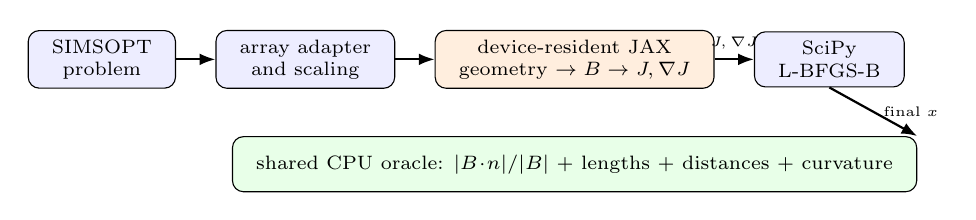
\begin{tikzpicture}[
  node distance=3mm and 5mm,
  box/.style={draw,rounded corners,align=center,minimum height=7mm,
              inner xsep=3mm,fill=blue!7,font=\scriptsize},
  metric/.style={draw,rounded corners,align=center,minimum height=7mm,
                 inner xsep=3mm,fill=green!9,font=\scriptsize},
  flow/.style={-{Latex[length=2mm]},thick}
]
\node[box] (problem) {SIMSOPT\\problem};
\node[box,right=of problem] (adapter) {array adapter\\and scaling};
\node[box,right=of adapter,fill=orange!13] (gpu) {device-resident JAX\\geometry $\to B\to J,\nabla J$};
\node[box,right=of gpu] (scipy) {SciPy\\L-BFGS-B};
\node[metric,below=6mm of gpu] (oracle) {shared CPU oracle:
  $|B\!\cdot\!n|/|B|$ + lengths + distances + curvature};
\draw[flow] (problem) -- (adapter);
\draw[flow] (adapter) -- (gpu);
\draw[flow] (gpu) -- node[above,font=\tiny] {$J,\nabla J$} (scipy);
\draw[flow] (scipy.south) -- node[right,font=\tiny] {final $x$} (oracle.north east);
\end{tikzpicture}
\caption{Implementation boundary and validation flow.  The expensive objective
stays on the GPU; both final designs are measured with one physical oracle.}
\label{fig:architecture}
\end{figure}

\section{Repository and baseline}

Development takes place on branch \code{gpu-native-objective} in the public
fork \url{https://github.com/PedroFranciscoGil/simsopt}.  It starts from
upstream commit
\href{https://github.com/hiddenSymmetries/simsopt/commit/c648630cfc5625863b291709c17015bcdcba13af}{\code{c648630cfc56}}
rather than from the fork's
stale default branch.  The upstream repository is
\url{https://github.com/hiddenSymmetries/simsopt}.

The existing implementation remains the compatibility oracle:
\begin{itemize}
  \item stage-two examples assemble an \code{Optimizable} objective and pass
        \code{J()} and \code{dJ()} to SciPy L-BFGS-B;
  \item Biot--Savart field evaluation and its analytic vector--Jacobian product
        use vectorized C++ kernels in \code{src/simsoptpp};
  \item field calculation is parallelized across coils with OpenMP;
  \item several curve quantities and regularizers already use JAX internally,
        but the complete objective crosses Python, NumPy, JAX, and C++
        boundaries and is not one device-resident computation.
\end{itemize}

All numerical comparisons will be made against a pinned upstream commit.  An
upstream update is a deliberate integration event, never an implicit change to
benchmark baselines.

\section{Scope}

\subsection{First supported problem}

The minimum useful GPU-native objective will support:
\begin{enumerate}
  \item Cartesian Fourier curves compatible with \code{CurveXYZFourier};
  \item unique base coils expanded through field-period and stellarator
        symmetries;
  \item scalar coil currents, including fixed and shared currents;
  \item a fixed target surface imported from \simsopt{};
  \item filamentary Biot--Savart evaluation on the surface;
  \item quadratic flux and, immediately afterward, normalized flux;
  \item curve length, curvature, mean-squared-curvature, arclength variation,
        coil--coil distance, and coil--surface distance terms;
  \item a scalar objective and an analytic/autodifferentiated gradient with
        respect to all free coil variables.
\end{enumerate}

\subsection{Deferred work}

The first milestone excludes VMEC/SPEC execution, finite-build coils,
self-force and torque, field-line tracing, moving plasma surfaces, distributed
multi-host execution, and a new optimizer.  These are important follow-on
targets but would prevent a small, testable first vertical slice.

\section{Design principles}

\begin{enumerate}
  \item \textbf{Functional numerical core.}  Kernels accept arrays and return
        arrays.  They do not mutate the \simsopt{} dependency graph.
  \item \textbf{Compatibility at the boundary.}  Adapter functions import an
        existing \simsopt{} problem into the GPU representation and export final
        variables back into the original objects.
  \item \textbf{Static shapes during optimization.}  Quadrature sizes, coil
        counts, and pair-list capacities remain fixed to avoid recompilation.
  \item \textbf{Device residency.}  Geometry, field, objective, and gradient
        execute without host callbacks or intermediate NumPy conversions.
  \item \textbf{Double precision first.}  Float64 is the reference mode.
        Float32 and mixed precision are optional, measured variants.
  \item \textbf{Memory-aware differentiation.}  Tiling, recomputation, and
        custom VJPs are preferred over materializing the full interaction
        tensor.
  \item \textbf{Performance follows evidence.}  A clear JAX implementation is
        built first.  Pallas, Triton, or custom CUDA is introduced only after a
        profiler identifies a kernel-level limitation.
\end{enumerate}

\section{Proposed package structure}

The initial implementation should be isolated enough to evolve quickly while
remaining inside the fork:
\begin{verbatim}
src/simsopt/gpu/
    __init__.py
    config.py             # precision and backend policy
    parameters.py         # flat variables and masks
    adapters.py           # SIMSOPT <-> array representation
    curves.py             # Fourier geometry and symmetry expansion
    biot_savart.py        # tiled field kernel and custom VJP
    flux.py               # flux residuals and objectives
    regularizers.py       # curve-local geometry terms
    distances.py          # tiled engineering distance terms
    objective.py          # composition and value-and-gradient API
    scipy.py              # flat SciPy bridge
tests/gpu/
    test_curves.py
    test_biot_savart.py
    test_flux.py
    test_regularizers.py
    test_objective.py
benchmarks/gpu/
    benchmark_objective.py
    sweep_gpu_tiles.py
    profile_gpu_objective.py
    problems.py
\end{verbatim}

The name \code{simsopt.gpu} is provisional.  Before exposing a public API, it
should be checked against upstream maintainers' naming and backend conventions.

\section{Work plan}

\subsection{Phase 0: reproducible CPU baseline}

\textbf{Tasks}
\begin{itemize}
  \item Define three benchmark classes: the minimal documented stage-two case,
        an engineering-regularized case, and a high-resolution stress case.
  \item Record coil count, Fourier order, coil quadrature, surface resolution,
        number of free variables, active objective terms, and thread count.
  \item Time curve evaluation, $B$, the Biot--Savart VJP, each regularizer, the
        combined $J/\nabla J$, and complete optimization.
  \item Store initial variables and reference outputs in compact test fixtures.
  \item Record hardware, compiler, BLAS, Python, JAX, and \simsopt{} versions.
\end{itemize}

\textbf{Exit criterion:} repeated CPU measurements are stable enough to detect
a 10\% regression, and all fixtures can be regenerated from documented
commands.

\subsection{Phase 1: array data model and Fourier curves}

Precompute Fourier basis matrices for $\gamma$, $\gamma'$, $\gamma''$, and
$\gamma^{(3)}$.  A curve evaluation then becomes a small collection of matrix
products.  Symmetry expansion will use fixed rotation/reflection matrices and
array broadcasting.  Free/fixed/shared current semantics and the ordering of
degrees of freedom must exactly match the adapter contract.

\textbf{Exit criterion:} base and symmetry-generated curve positions and their
first three derivatives agree with \simsopt{} in float64, and JVP/VJP tests pass
for random coefficients and several Fourier orders.

\subsection{Phase 2: GPU Biot--Savart forward kernel}

Implement
\[
 \mathbf B(\mathbf x_i)=\frac{\mu_0}{4\pi}
 \sum_k I_k\int_0^1
 \frac{(\gamma_k-\mathbf x_i)\times\gamma'_k}
      {\lVert\gamma_k-\mathbf x_i\rVert^3}\,d\phi
\]
using target and source tiling.  The first version will use JAX primitives and
fixed chunk sizes selected by an autotuning benchmark.  It must reduce partial
fields without constructing an array with dimensions
\code{targets x coils x quadrature x 3} for the complete problem.

\textbf{Exit criterion:} field values agree with the C++ implementation at all
benchmark resolutions, memory scales according to the selected tile size, and
the profiler shows no host transfer inside the compiled field call.

\subsection{Phase 3: memory-bounded reverse pass}

The ordinary reverse-mode implementation remains the reference.  Setting
\code{vjp\_mode="custom"}, now the default, supplies a custom VJP that
analytically contracts the field cotangent with each target--source pair.  It
returns cotangents for target points, curve positions, curve tangents, and
currents; it stores only the primal inputs and recomputes pair interactions in
source and target tiles rather than retaining the autodiff tape or a complete
interaction tensor.  Random padded-shape tests compare all four cotangents
against full-tensor autodiff, and a centered directional-derivative test covers
their joint contraction.  Because JAX custom VJPs do not provide a forward-mode
rule, the ordinary field function remains available for JVP use.

The autotuner treats reverse-pass mode as another candidate dimension and
always confirms both the best ordinary-autodiff result and the original
baseline.  NVIDIA results in Section~\ref{sec:first-profile} motivated promotion
of the custom VJP for composed reverse-mode objectives.  The ordinary field
function remains the public path for forward-mode use.  Selection uses total
value-and-gradient time and peak memory, not forward time alone.

\textbf{Exit criterion:} directional derivatives pass centered finite-
difference/Taylor tests and agree with the existing analytic VJP over random and
near-converged coil sets.

\subsection{Phase 4: flux and regularizers}

Quadratic and normalized flux, length, and the curve-local regularizers are
complete.  The distance milestone now adds SIMSOPT-equivalent coil--coil and
coil--surface hinge penalties.  Coil pairs are the exact static symmetry set
$j<i$, $j<n_{\rm base}$; evaluating this complete set is equivalent to the CPU
candidate filter because rejected pairs contribute exactly zero.  Curve pairs
are accumulated in a compiled loop.  Surface interactions use padded target
tiles with rematerialization, avoiding a full
\code{coils x curve points x surface points x 3} reverse-mode tape.

Independent fixtures compare both distance values and position/tangent
gradients with the existing JAX definitions.  The complete composed objective,
including linear length and all engineering penalties, matches the SIMSOPT CPU
oracle in both reverse-pass modes.  The GPU test suite contains 71 passing
tests.  Historical scopes remain available; production now selects
\code{full-engineering} and reports no deferred terms.

Thresholded penalties should be tested at and near their nondifferentiable
activation points.  A smooth approximation may be offered later, but it must
not silently replace existing semantics.

\textbf{Exit criterion:} distance terms pass objective and gradient parity
before the complete production-objective benchmark is enabled.

\subsection{Phase 5: integrated objective and SciPy bridge}

The integrated value-and-gradient function and SciPy bridge are complete.  The
coil-specific bridge packs variables in SIMSOPT's exact
order---free currents followed by Fourier coefficients---while fixed currents
remain device constants.  Compilation and warm-up precede timing; each solver
call transfers only the flat vector, scalar, and gradient.  A trajectory harness
runs identical L-BFGS-B settings through CPU and GPU paths, records evaluations
and accepted iterates, and rechecks both final designs with the CPU metric
oracle.  Section~\ref{sec:trajectory} records the production result.

The bridge also supports an explicit diagonal current transform
$I=s_I z_I$, with $\nabla_{z_I}J=s_I\nabla_IJ$.  Its default $s_I=1$ preserves
the original coordinates; the convergence workflow uses $s_I=10^5$ amperes so
currents and curve coefficients are numerically comparable without changing the
physical objective.

Optimization artifacts now use a versioned final-metric contract.  CPU and GPU
designs each retain mean, RMS, and maximum $|B\cdot n|/|B|$, per-coil length,
maximum and mean-squared curvature, minimum coil--coil and coil--surface
distance, current values, configured limits, signed margins, and violations.
Both snapshots are recomputed through the same CPU oracle.
For visual inspection, each final design also exports a surface VTS with signed
and absolute $(B\cdot n)/|B|$ fields and a VTU containing all physical coils.

\textbf{Exit criterion:} equivalent metrics, equal evaluation counts, and the
GPU speed advantage are demonstrated over a 25-iteration trajectory.  A longer
run is still required to compare converged stationary points.

\subsection{Phase 6: profiling and kernel specialization}

Use JAX traces and a GPU profiler to classify time as compilation, dispatch,
compute, reduction, or transfer.  Optimize only dominant kernels.  Candidate
actions include changing layouts and tile sizes, fusing flux reduction into
Biot--Savart, rematerializing the reverse pass, or implementing a Pallas/custom
kernel.  Each optimization requires a benchmark and a regression test.

\textbf{Exit criterion:} the production-sized benchmark meets the performance
gate in Section~\ref{sec:gates}, or the measured bottleneck and reason for a
no-go decision are documented.

\subsection{Phase 7: GPU-native solver experiments}

After objective completion, compare the unchanged SciPy trajectory with:
\begin{itemize}
  \item maintained Optax L-BFGS with a zoom line search for unconstrained cases;
  \item full BFGS when the variable count makes its $O(n^2)$ state affordable;
  \item a reviewed/vendor-pinned L-BFGS-B implementation for true box bounds;
  \item matrix-free Gauss--Newton or Levenberg--Marquardt on a residual-form
        objective.
\end{itemize}
Optimizer comparisons must report wall time, number of physics evaluations,
convergence status, constraint violations, and final engineering metrics.

\section{Correctness and performance gates}\label{sec:gates}

\begin{longtable}{p{0.26\textwidth}p{0.66\textwidth}}
\toprule
Gate & Initial acceptance condition \\
\midrule
\endhead
Field parity & Float64 $B$ agrees with the CPU reference using
  $\mathrm{rtol}\leq10^{-9}$ and a scale-appropriate absolute tolerance. \\
Objective parity & Each objective component and the combined objective meet
  documented absolute and relative tolerances over initial, random, and
  converged geometries. \\
Gradient parity & Analytic GPU and CPU gradients agree with
  $\mathrm{rtol}\leq10^{-7}$ away from threshold kinks; discrepancies are also
  checked by directional derivatives. \\
Taylor behavior & Centered directional errors display the expected second-order
  slope before floating-point saturation. \\
Residency & No host callback or intermediate device-to-host transfer occurs
  inside the steady-state value-and-gradient trace. \\
Memory & Peak memory is bounded by configured tiles and fits the reference GPU
  with at least 20\% operational headroom. \\
Speed & After compilation, combined $J/\nabla J$ is at least $3\times$ faster
  than the tuned CPU baseline on the production-sized benchmark.  Small cases
  are allowed to favor the CPU. \\
Optimization & From identical initial data, the GPU backend produces equivalent
  or better flux and engineering metrics without increasing physics evaluations
  by more than 10\% under the same SciPy solver configuration. \\
\bottomrule
\end{longtable}

Tolerances are starting values, not universal constants.  They will be scaled
for singular or nearly singular geometries, but any relaxation must be recorded
with the affected fixture and physical reason.

\section{Benchmark protocol}

JAX execution is asynchronous, so all timed regions must synchronize their
outputs.  Compilation and execution are reported separately.  Each benchmark
will include warm-up, multiple repetitions, median and dispersion, peak device
memory, and a saved machine-readable result.  CPU comparisons must use a fixed
OpenMP thread count and affinity configuration.

The benchmark matrix includes:
\begin{itemize}
  \item CPU C++/OpenMP versus JAX CPU versus JAX GPU;
  \item float64 as the primary comparison, with optional float32 and mixed
        precision experiments;
  \item field only, VJP only, combined objective/gradient, and complete solve;
  \item scaling in surface points, coil quadrature, physical coils, and free
        variables;
  \item cold-start time and amortized time for one, ten, and many solves.
\end{itemize}

For every optimization run, the machine-readable artifact must contain separate
CPU and GPU final snapshots.  Timing or objective decrease alone is never
sufficient: normalized normal-field quality and every active physical
constraint must be retained even when a run stops at its iteration limit.

The target accelerator should have credible float64 throughput.  Consumer GPUs
may still be useful for development and batched float32 experiments, but they
must not define the primary scientific-performance conclusion.

\section{First NVIDIA profile result}\label{sec:first-profile}
\begingroup\footnotesize

The first external GPU run was captured on 10 September 2026 from repository
revision \code{127e7a50c3ad} using the documented minimal problem.  The device
was an NVIDIA Tesla T4 with 15,360 MiB of physical memory; JAX 0.11.1 selected
the CUDA backend and enabled float64.  The problem contained four base coils,
16 symmetry-expanded physical coils, 75 quadrature points per curve, a
$32\times32$ target surface, and 136 differentiated variables.  Target and
source tile sizes were 128 and 256, respectively.

Compilation took $3.384\ \mathrm{s}$ and ten synchronized calls had a
$21.767\ \mathrm{ms}$ median, a $21.656$--$21.908\ \mathrm{ms}$ range, and
0.369\% coefficient of variation.  The objective absolute error was
$6.94\times10^{-18}$ and gradient relative errors were below
$5.58\times10^{-16}$.  Peak device memory was 150.27 MiB, only 1.34\% of the
JAX limit.  The trace contained no
host--device copies inside the objective, but its 40 tile iterations produced
130 device-to-device copies and 148 command-buffer executions per call.  This
passed the minimal-case parity, residency, and memory gates and identified
launch granularity and reverse-pass state movement as optimization targets;
without a timed CPU baseline it did not establish a speedup.

\subsection{Automated tile and reverse-pass sweeps}

A second T4 run from revision \code{63a6631f3146} screened all 25 combinations
of five target and five source tile sizes.  All candidates passed the objective
and gradient gates and identified $512\times1200$ as the best ordinary-autodiff
configuration.  A third run from revision \code{45bb1e86fac7} jointly screened
the same tiles with ordinary autodiff and the custom VJP.  All 50 candidates
passed parity; the leading candidates and reference paths were confirmed with
ten synchronized evaluations after three warm-up calls.

\begin{figure}[htbp]
\centering
\begin{minipage}{0.48\textwidth}
\centering
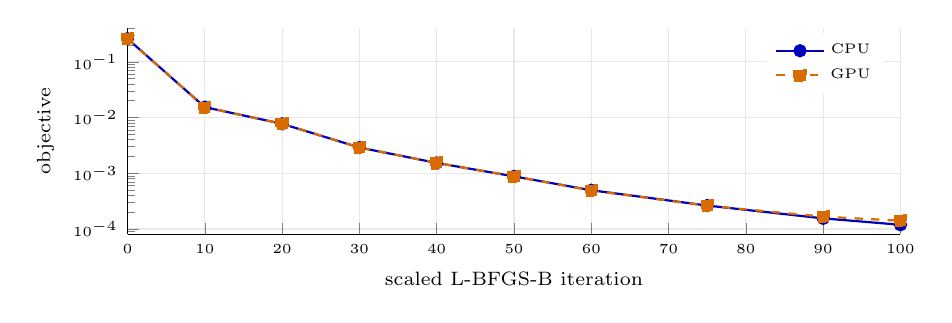
\begin{tikzpicture}
\begin{axis}[
  width=0.94\linewidth,height=4.2cm,
  xlabel={scaled L-BFGS-B iteration},ylabel={objective},ymode=log,
  xmin=0,xmax=100,ymin=8e-5,ymax=4e-1,
  tick label style={font=\tiny},label style={font=\scriptsize},
  grid=major,grid style={gray!18},axis lines*=left,
  legend style={font=\tiny,draw=none,at={(0.98,0.98)},anchor=north east}
]
\addplot[blue!75!black,thick,mark=*] coordinates {
  (0,0.25950643) (10,0.01535511) (20,0.00771889)
  (30,0.00289598) (40,0.00153308) (50,0.00087949)
  (60,0.00049620) (75,0.00026348) (90,0.00015517)
  (100,0.00011914)};
\addlegendentry{CPU}
\addplot[orange!85!black,thick,dashed,mark=square*] coordinates {
  (0,0.25950643) (10,0.01535511) (20,0.00771889)
  (30,0.00289598) (40,0.00153307) (50,0.00088044)
  (60,0.00049206) (75,0.00026143) (90,0.00016672)
  (100,0.00014075)};
\addlegendentry{GPU}
\end{axis}
\end{tikzpicture}
\end{minipage}%
\begin{minipage}{0.48\textwidth}
\centering
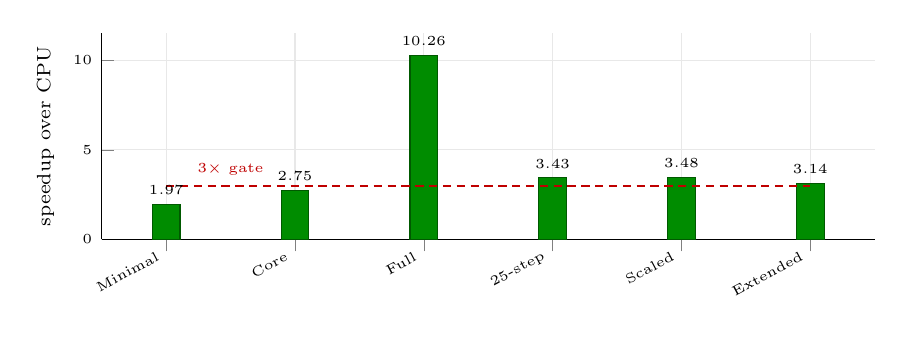
\begin{tikzpicture}
\begin{axis}[
  width=0.94\linewidth,height=4.2cm,ybar,bar width=10pt,
  ylabel={speedup over CPU},
  symbolic x coords={Minimal,Core,Full,25-step,Scaled,Extended},xtick=data,
  xticklabel style={rotate=28,anchor=east,font=\tiny},
  tick label style={font=\tiny},label style={font=\scriptsize},
  ymin=0,ymax=11.5,enlarge x limits=0.10,
  nodes near coords,nodes near coords style={font=\tiny},
  grid=major,grid style={gray!18},axis lines*=left
]
\addplot[fill=green!55!black,draw=green!35!black]
 coordinates {(Minimal,1.974) (Core,2.752) (Full,10.256)
              (25-step,3.433) (Scaled,3.476) (Extended,3.141)};
\draw[densely dashed,red!75!black,thick]
  (axis cs:Minimal,3) -- (axis cs:Extended,3)
  node[pos=.10,above,font=\tiny] {$3\times$ gate};
\end{axis}
\end{tikzpicture}
\end{minipage}
\caption{Measured Tesla T4 progress.  Left: scaled CPU/GPU objective histories
remain close initially and separate late in the nonconverged run.  Right: warm speedups
for the minimal objective, production core, full engineering objective,
25-step solve, 100-step scaled solve, and 300-step extended solve.}
\label{fig:performance}
\end{figure}

The custom winner is $1.565\times$ faster than tuned autodiff,
$2.692\times$ faster than the original configuration, and provisionally
$1.974\times$ faster than the CPU-pinned one-thread reference.  Its confirmation
coefficient of variation is 2.31\%; a separate profile reproduced a
$7.996\ \mathrm{ms}$ median with 0.393\% variation.  Compilation takes
$1.567\ \mathrm{s}$, equivalent to approximately 196 steady evaluations.
Float64 parity remains at rounding scale: objective absolute error is
$6.94\times10^{-18}$ and curve- and current-gradient relative errors are
$5.32\times10^{-16}$ and $1.92\times10^{-16}$.

The one-tile custom trace contains no memcpy event and only one command-buffer
execution per evaluation, down from 130 copies and 148 command buffers in the
original path.  Across three calls, GPU-stream span is $23.85\ \mathrm{ms}$ and
summed GPU activity is $23.14\ \mathrm{ms}$.  Peak memory is 100.14 MiB, 0.90\%
of the JAX device limit and 61\% below the 256.03 MiB tuned-autodiff profile.
The dominant events are now the inverse-distance power and reduction kernels.

\textbf{Decision.}  Promote the custom VJP to the default for composed
reverse-mode objectives and use $1024\times1200$ for this minimal T4 case.
Keep conservative library-wide tile defaults until engineering and stress
workloads and a stronger float64 accelerator have been swept.  Keep ordinary
\code{biot\_savart\_field} for forward-mode JVPs.  The next gate is scaling on
larger workloads; low-level kernel specialization will follow only if their
profiles show the same arithmetic bottleneck.  The production-size test and a
tuned CPU baseline remain necessary before evaluating the $3\times$ speed gate.

\subsection{Production-scale T4 result}

The production workflow ran on 11 September 2026 from revision
\code{f01331c1b613}.  Its six base coils, 24 physical coils, Fourier order 12,
180 quadrature points, and $128\times128$ half-period surface produce 70,778,880
target--source interactions and 456 differentiated variables.  All 25 custom-
VJP tile candidates completed and passed parity.  Confirmation selected a
$512\times4320$ tile---32 target blocks and one unpadded source block---at a
$214.346\ \mathrm{ms}$ median with 0.214\% coefficient of variation.  The
one-thread CPU median was $589.955\ \mathrm{ms}$ with 2.02\% variation, giving
a $2.752\times$ speedup: 8.26\% short of the $3\times$ gate.

An independent profile reproduced $216.475\ \mathrm{ms}$ with 0.281\%
variation.  Compilation took $2.863\ \mathrm{s}$, or 13.4 steady evaluations.
Objective error was zero and the worst confirmed gradient relative error was
$1.25\times10^{-14}$.  Peak profile memory was 128.15 MiB (1.15\% of the JAX
limit); even the complete sweep peaked at only 541.18 MiB.  Relative to the
minimal run, interactions increased $57.6\times$ while GPU latency increased
only $26.86\times$, improving interaction throughput by $2.144\times$.

The trace contained no host--device transfer.  Its five dominant arithmetic
and reduction kernels accounted for 99.49\% of GPU activity.  Device-to-device
copies consumed only $0.061\ \mathrm{ms}$ per call and command-buffer host time
only $1.50\ \mathrm{ms}$, so dispatch optimization cannot close the remaining
gap.  At target tile 512, source-tail padding is material: a 4096-source tile
executes two full blocks and screened at $397.4\ \mathrm{ms}$, versus
$209.9\ \mathrm{ms}$ for the exact 4320-source tile.

\textbf{Decision.}  Accept the production core's correctness, scaling,
residency, and memory results, but do not mark the performance gate complete.
Retain per-workload autotuning and judge specialization using the complete
objective.

\subsection{Complete engineering-objective T4 result}

The complete objective ran on the same T4 class on 11 September 2026 from
revision \code{0799eee2}.  It includes flux, linear length, coil--coil and
coil--surface distances, thresholded curvature, and mean-squared-curvature;
no benchmark term is deferred.  All 25 configurations passed parity.  Ten-call
confirmation selected $1024\times4320$ at a $309.192\ \mathrm{ms}$ median and
0.128\% variation.  The independent profile recorded $305.288\ \mathrm{ms}$
and 0.250\% variation.  Against the seven-call one-thread CPU median of
$3.17113\ \mathrm{s}$, the confirmed speedup is $10.256\times$.

Compilation took $4.731\ \mathrm{s}$.  Objective error was zero; curve and
current gradient relative errors were $6.01\times10^{-16}$ and
$1.31\times10^{-16}$.  Peak profile memory was 336.87 MiB, 3.01\% of the JAX
limit; the complete sweep peaked at 541.69 MiB.  Thus every production gate,
including the $3\times$ speed gate, passed.  Adding all engineering terms raised
GPU time only $1.442\times$ relative to the earlier core confirmation, whereas
CPU time rose $5.375\times$; the full objective therefore exposes the GPU's
main practical advantage.

Across three traced calls, GPU activity was $914.59\ \mathrm{ms}$ over a
$921.37\ \mathrm{ms}$ stream span, with no host--device copy.  Biot--Savart
forward/reverse used about $153.5\ \mathrm{ms}$ per call, tiled coil--surface
distance about $131.8\ \mathrm{ms}$, and the 123-pair coil--coil loop about
$17\ \mathrm{ms}$.  The pair loop contributes most of the 422 command-buffer
executions and $11.0\ \mathrm{ms}$ host command-buffer time per call, but this
is only 3.6\% of latency.

\textbf{Decision.}  Accept the all-pairs JAX implementation as the production
reference and do not introduce Pallas/Triton or dynamic neighbor lists now.
The measured objective has ample correctness, memory, and speed margin.  Pair
batching remains a low-risk later optimization.

\subsection{SciPy L-BFGS-B trajectory result}\label{sec:trajectory}

Revision \code{8c78474e} compared identical SciPy L-BFGS-B settings for the
complete stress problem: 455 free variables, \code{maxcor=300}, and a
25-iteration cap.  CPU and GPU each used 43 value/gradient evaluations and
accepted 25 iterates before stopping at that cap.  The GPU objective initially
matched exactly and its gradient relative error was $6.01\times10^{-16}$.
Across accepted iterates, maximum objective error was $1.12\times10^{-10}$ and
maximum curve-state relative error $2.17\times10^{-9}$; free-current trajectories
were identical.  Final objectives were $0.004628353933$ and $0.004628353872$,
a $6.06\times10^{-11}$ difference.  The worst relative discrepancy among all
CPU-oracle engineering metrics was $4.55\times10^{-7}$.

CPU optimization took $44.042\ \mathrm{s}$ and GPU optimization
$12.828\ \mathrm{s}$, a $3.433\times$ end-to-end solver speedup excluding the
one-time $6.637\ \mathrm{s}$ compilation.  Including compilation gives
$2.263\times$ for this short run; the compile cost breaks even after roughly
ten evaluations.  The objective fell $56.1\times$, but neither run converged:
the final gradient norm was 0.221 and both returned the iteration-limit status.

\textbf{Scaled convergence update.}  Revision \code{9901d14b} used
$s_I=10^5$ on the same T4.  CPU and GPU started identically; their objective
histories remained close through roughly 40 iterations, then followed different
floating-point-sensitive paths.  Both reached the 100-iteration cap: CPU used 140 evaluations and ended
at $J=1.19135\times10^{-4}$ with $\lVert\nabla J\rVert=3.22\times10^{-3}$;
GPU used 152 and reached $1.40748\times10^{-4}$ with
$7.28\times10^{-3}$.  Wall times were 157.637 and 45.346 seconds, a
$3.476\times$ warm speedup and $3.100\times$ including 5.497 seconds of
compilation.

\begin{center}
\begin{tabular}{lrrr}
\toprule
Final physical metric & Limit & CPU & GPU \\
\midrule
Mean $|B\cdot n|/|B|$       & --    & 0.008226 & 0.008988 \\
RMS $|B\cdot n|/|B|$        & --    & 0.010406 & 0.011544 \\
Maximum $|B\cdot n|/|B|$    & --    & 0.037545 & 0.037477 \\
Minimum coil--coil distance & 0.100 & 0.099830 & 0.099287 \\
Minimum coil--surface distance & 0.300 & 0.292981 & 0.292884 \\
Maximum curvature           & 5.000 & 9.269878 & 6.368665 \\
Maximum mean-squared curvature & 5.000 & 7.305160 & 7.604921 \\
Total base-coil length      & --    & 29.020967 & 29.082666 \\
\bottomrule
\end{tabular}
\end{center}

\textbf{Decision.}  The speed and evaluation-budget gates pass, but stationarity,
full-trajectory parity, and final-metric parity do not.  Neither design satisfies
all penalty thresholds.  This is not a native-solver comparison.  The next run
now extends the cap to 300: backend validation uses the first 25 iterates, while
solver acceptance uses stationarity, final normalized-field quality, and
constraint violations rather than identical late iterates.  It also exports
both final surfaces and coil sets for ParaView.

\subsection{Extended convergence and final-field result}

The 300-iteration workflow ran on 11 September 2026 from revision
\code{c7a622674050} on a Tesla T4 with 15,360 MiB.  The supplied archive has
SHA-256 digest
\nolinkurl{3ec3be9f43704a858087a48e0e32bb9bde954ea1ac307cdb3a7317642ce2f139}.
It contains schema-3 JSON and nonempty CPU/GPU surface and coil VTK files.  The
stress problem has 455 optimization variables, 4,320 source points, 16,384
surface points, $1024\times4320$ custom-VJP tiles, and current scale $10^5$ A.

Initial float64 value and gradient parity passed at zero and
$6.01\times10^{-16}$ error, respectively.  Over the first 25 accepted iterates,
maximum objective error was $3.08\times10^{-11}$ and maximum curve-state
relative error $5.13\times10^{-10}$, comfortably inside the backend contract.
Thereafter the nonconvex trajectories separated.  Figure~\ref{fig:extended-convergence}
shows that both continued to reduce the objective; the GPU path became better
from iteration 161 onward.

\begin{figure}[htbp]
\centering
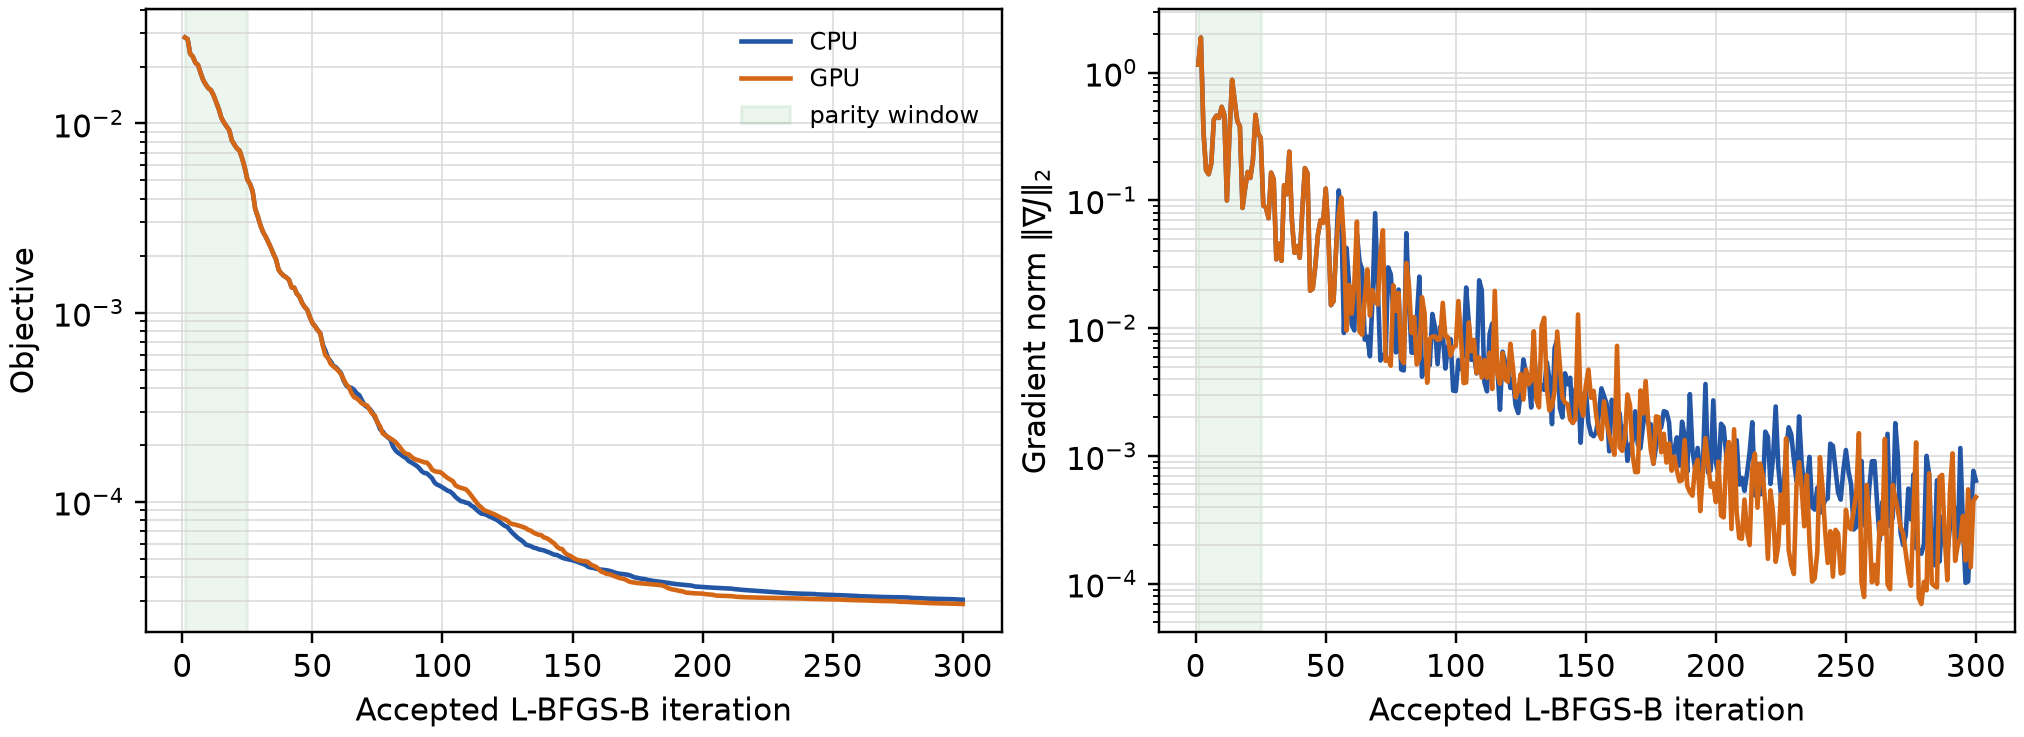
\includegraphics[width=\textwidth]{figures/extended_convergence.png}
\caption{Extended T4 convergence from the archived accepted-iterate histories.
The shaded region is the 25-iteration backend-parity window.  Later differences
are solver-path differences; both gradients remain above the stationarity gate.}
\label{fig:extended-convergence}
\end{figure}

\begin{center}
\begin{tabular}{lrr}
\toprule
Optimization measurement & CPU & GPU \\
\midrule
Iterations & 300 & 300 \\
Physics evaluations & 378 & 436 \\
Wall time (s) & 420.056 & 133.737 \\
Median evaluation time (s) & 1.04475 & 0.30133 \\
Final objective & $3.03442\times10^{-5}$ & $2.88096\times10^{-5}$ \\
Final gradient norm & $6.40029\times10^{-4}$ & $4.76719\times10^{-4}$ \\
\bottomrule
\end{tabular}
\end{center}

The warm optimization speedup is $3.141\times$, and $2.989\times$ including
the $6.778$ s compilation.  Per-evaluation medians differ by $3.467\times$.
However, the GPU path required 15.34\% more physics evaluations, missing the
10\% evaluation-budget gate.  Both solvers stopped at the iteration cap and
missed the $10^{-5}$ stationarity gate.  Thus the result establishes useful
end-to-end acceleration, but not converged-solver equivalence.

\begin{center}
\begin{tabular}{lrrr}
\toprule
Final CPU-oracle metric & Limit & CPU & GPU \\
\midrule
Mean $|B\cdot n|/|B|$ & -- & 0.000973 & 0.000730 \\
RMS $|B\cdot n|/|B|$ & -- & 0.001215 & 0.000917 \\
Maximum $|B\cdot n|/|B|$ & -- & 0.004286 & 0.003241 \\
Minimum coil--coil distance & 0.100 & 0.099917 & 0.099912 \\
Minimum coil--surface distance & 0.300 & 0.299702 & 0.298478 \\
Maximum curvature & 5.000 & 5.323129 & 5.478761 \\
Maximum mean-squared curvature & 5.000 & 5.126890 & 5.166965 \\
Total base-coil length & -- & 29.239720 & 28.210168 \\
\bottomrule
\end{tabular}
\end{center}

The GPU final design improves mean, RMS, and maximum normalized normal field by
25.0\%, 24.5\%, and 24.4\%, so the normal-field quality gate passes.  It does
not pass the relative engineering-quality gate: its coil--surface deficit is
1.522 mm versus 0.298 mm on CPU, maximum curvature violation is 0.479 versus
0.323, and mean-squared-curvature violation is 0.167 versus 0.127.  Neither
design is strictly feasible.  The raw objective favors the GPU design partly
through a trade toward flux and shorter coils; this is consistent with the
$10^{-6}$ curvature-family weights being too small to enforce the stated
engineering limits.

The VTS files contain signed and absolute $(B\cdot n)/|B|$, raw $B\cdot n$,
and $|B|$ at all 16,384 surface points; the VTU files contain all 24 physical
coils and their currents.  Figure~\ref{fig:extended-field} visualizes the signed
surface arrays.  The GPU design has smaller absolute error at 61.5\% of points.
The maps have signed correlation 0.648 and relative $L^2$ difference 0.772;
these compare two different final coil sets and must not be interpreted as a
fixed-state backend-parity error.

\begin{figure}[htbp]
\centering
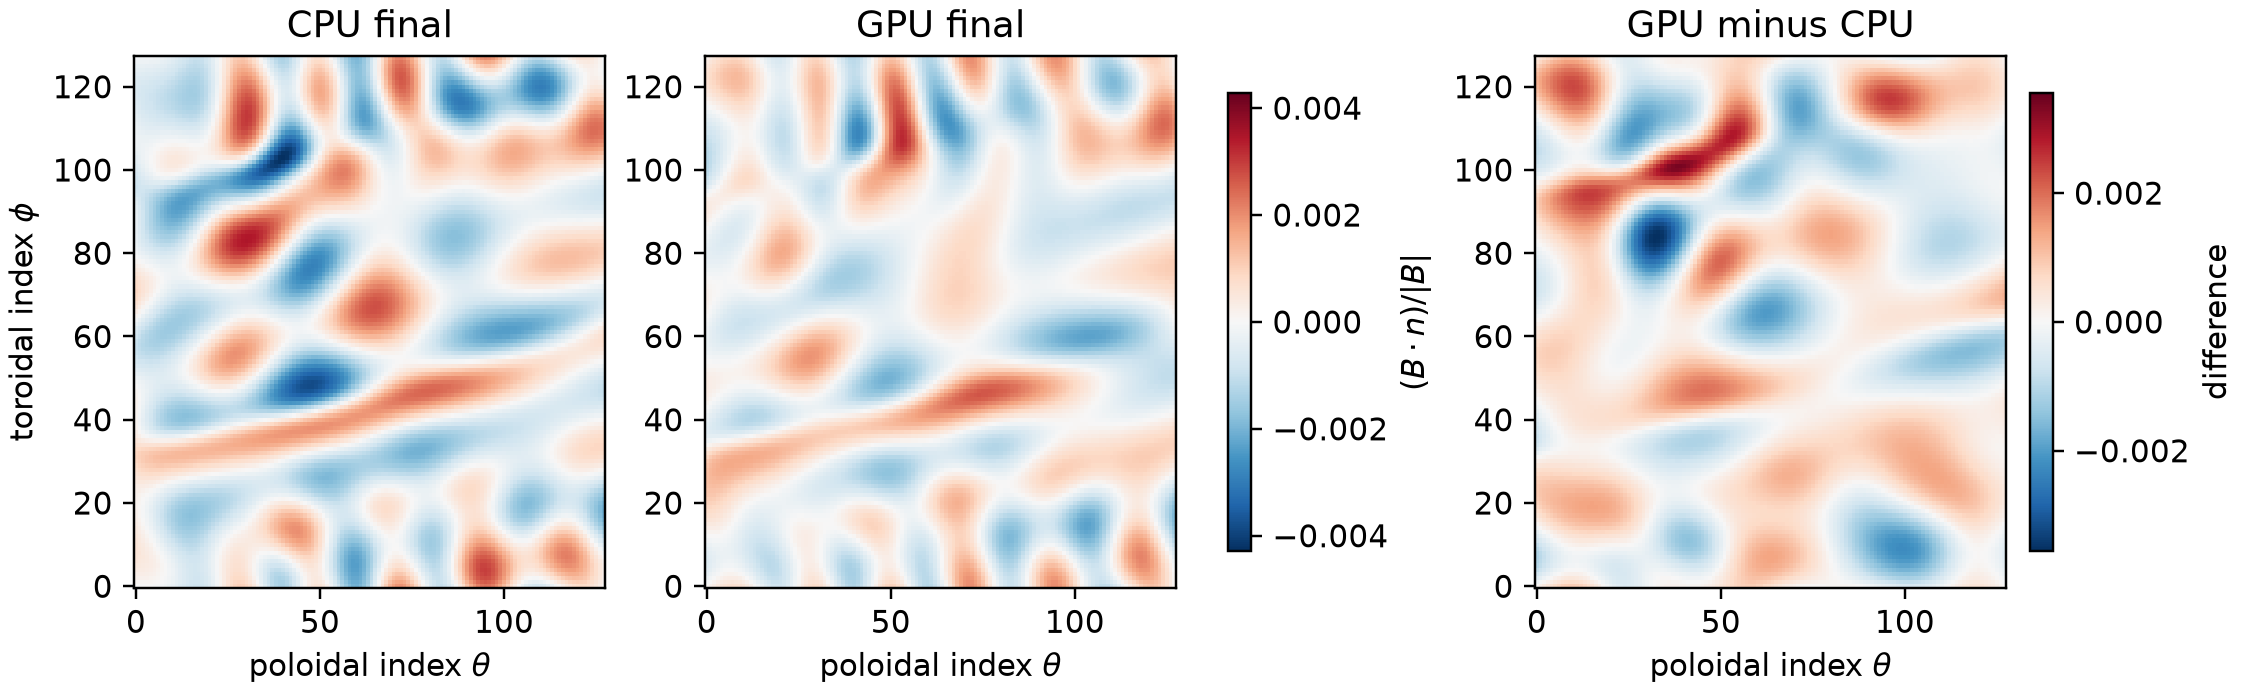
\includegraphics[width=\textwidth]{figures/extended_surface_field.png}
\caption{Archived final normalized normal-field maps.  CPU and GPU panels share
one color scale; the difference panel has its own symmetric scale.  The visible
pattern change is consistent with the 3.24\% final curve-state difference after
the two L-BFGS-B paths separated.}
\label{fig:extended-field}
\end{figure}

\textbf{Decision.}  Accept the GPU objective's parity, VTK export, final
normal-field quality, and $3\times$ warm end-to-end performance.  Do not accept
the optimization milestone as converged or engineering-feasible.  Merely raising
the iteration cap again is not the next experiment.  First add an absolute
feasibility gate, run a documented penalty-weight continuation, and sweep
L-BFGS memory/line-search settings while retaining the first-25-iterate backend
check.  A device-native L-BFGS implementation remains deferred until a common
solver configuration reaches stationarity and feasibility; otherwise it would
confound a solver redesign with an unresolved objective-conditioning problem.

\subsection{Absolute-feasibility workflow implementation}

That next experiment is now implemented, but no new NVIDIA measurements are
claimed until its Colab archive is returned.  Comparison schema~4 adds explicit
absolute violation tolerances: $10^{-4}$~m for both minimum-distance deficits
and $10^{-3}$ for maximum-curvature and maximum-mean-squared-curvature excesses.
It also records \code{maxls}, optional \code{ftol}/\code{gtol}, the common
engineering-weight multiplier, and both final physical variable vectors.  The
complete CPU-oracle metric snapshots and visualization contract remain
mandatory.

\begin{figure}[htbp]
\centering
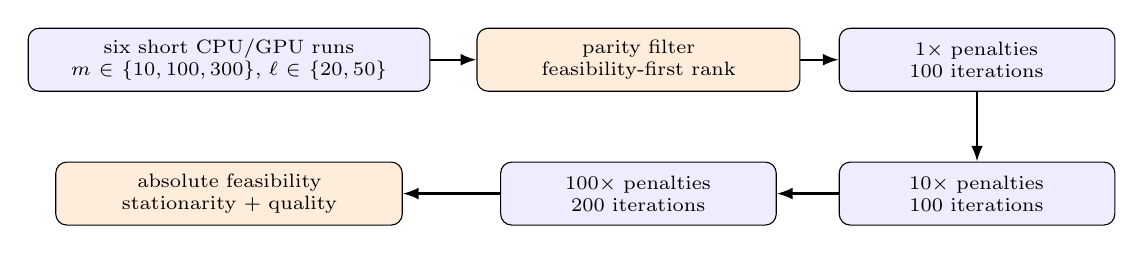
\begin{tikzpicture}[
  box/.style={draw,rounded corners,align=center,minimum height=8mm,
              inner xsep=4mm,fill=blue!7,font=\scriptsize},
  decision/.style={draw,rounded corners,align=center,minimum height=8mm,
              inner xsep=4mm,fill=orange!14,font=\scriptsize},
  flow/.style={-{Latex[length=2mm]},thick}
]
\node[box,text width=43mm] (sweep) at (0,0) {six short CPU/GPU runs\\
  $m\in\{10,100,300\}$, $\ell\in\{20,50\}$};
\node[decision,text width=33mm] (rank) at (5.2,0)
  {parity filter\\feasibility-first rank};
\node[box,text width=27mm] (p1) at (9.5,0)
  {$1\times$ penalties\\100 iterations};
\node[box,text width=27mm] (p10) at (9.5,-1.7)
  {$10\times$ penalties\\100 iterations};
\node[box,text width=27mm] (p100) at (5.2,-1.7)
  {$100\times$ penalties\\200 iterations};
\node[decision,text width=36mm] (gate) at (0,-1.7)
  {absolute feasibility\\stationarity + quality};
\draw[flow] (sweep) -- (rank);
\draw[flow] (rank) -- (p1);
\draw[flow] (p1) -- (p10);
\draw[flow] (p10) -- (p100);
\draw[flow] (p100) -- (gate);
\end{tikzpicture}
\caption{Implemented solver-setting sweep and synchronized penalty
continuation.  CPU and GPU always start a stage from the same physical vector;
only the final stage exports the two VTS/VTU design pairs.}
\label{fig:feasibility-workflow}
\end{figure}

The solver sweep evaluates the Cartesian product of L-BFGS memory
\code{maxcor} and line-search budget \code{maxls}.  A candidate is eligible only
after initial and first-25-iterate parity checks.  Its lexicographic rank is the
number of failed absolute constraints, maximum and sum of tolerance-normalized
violations, maximum final gradient norm, worst CPU/GPU normalized-normal-field
RMS, and combined function-evaluation count.  This explicitly prevents a fast
but physically unacceptable candidate from winning.

Penalty continuation uses default multipliers $1,10,100$ with iteration budgets
$100,100,200$.  All four inequality weights---coil--coil distance,
coil--surface distance, curvature, and mean-squared curvature---change together;
thresholds, flux, length weight, resolution, and current scaling do not.  At a
stage boundary, the endpoint with the better feasibility-first rank supplies
one physical restart vector to \emph{both} backends.  Every stage stores both
final objective/field/constraint snapshots and its selected restart provenance.
The aggregate acceptance requires an actual GPU, initial and early parity at
every stage, final absolute feasibility, stationary convergence, final
normal-field quality, the final evaluation-budget gate, and both final-stage
and aggregate $3\times$ warm speed.

The checked-in Colab notebook executes 69 GPU tests, performs the six-candidate
sweep, feeds its winner into the three-stage continuation, validates all four
final VTK files, and downloads one self-contained archive even when a scientific
gate fails.  A two-stage, one-iteration CPU-fallback smoke test has exercised
restart serialization, schema~4, absolute-gate reporting, aggregate summaries,
and VTS/VTU export; its timing and feasibility outcome are deliberately not
treated as production evidence.

\textbf{Decision.}  Run the new Colab workflow unchanged and analyze the
returned archive before changing tolerances or implementing a native solver.
If continuation attains feasibility and stationarity, the next controlled
experiment is a device-resident L-BFGS implementation against this SciPy
baseline.  If it does not, the next implementation should be explicit
constraint handling (most likely an augmented Lagrangian), not still larger
penalty weights.

\subsection{Feasibility sweep and continuation result}

The workflow ran on 11 September 2026 from revision \code{82fd11a62c49} on an
NVIDIA Tesla T4 with 15,360~MiB.  The supplied archive has SHA-256 digest
\nolinkurl{e785bb94c205e7bbee65b173a3da6767f6e15bd04ad831cc22bfd45d26254964}.
It contains both version-1 workflow summaries, all six schema-4 sweep results,
all three schema-4 continuation results and restart vectors, and four nonempty
final VTK files.

All six 25-iteration sweep candidates passed initial and early-trajectory
parity and exceeded the $3\times$ warm speed gate, but none was stationary or
absolutely feasible at that short horizon.  The \code{maxls=20} and 50 paths
were materially identical, so the larger line-search budget was never used.
Likewise, \code{maxcor=100} and 300 were identical: at 25 iterations both
values exceed the available correction history.  The feasibility-first rank
therefore selected \code{maxcor=100,maxls=20} as the first member of a tie, not
as evidence that 100 is intrinsically better than 300.  \code{maxcor=10}
finished with a slightly larger worst normalized violation.  Future memory
sweeps must use a horizon at least as long as the largest history candidate.

\begin{figure}[htbp]
\centering
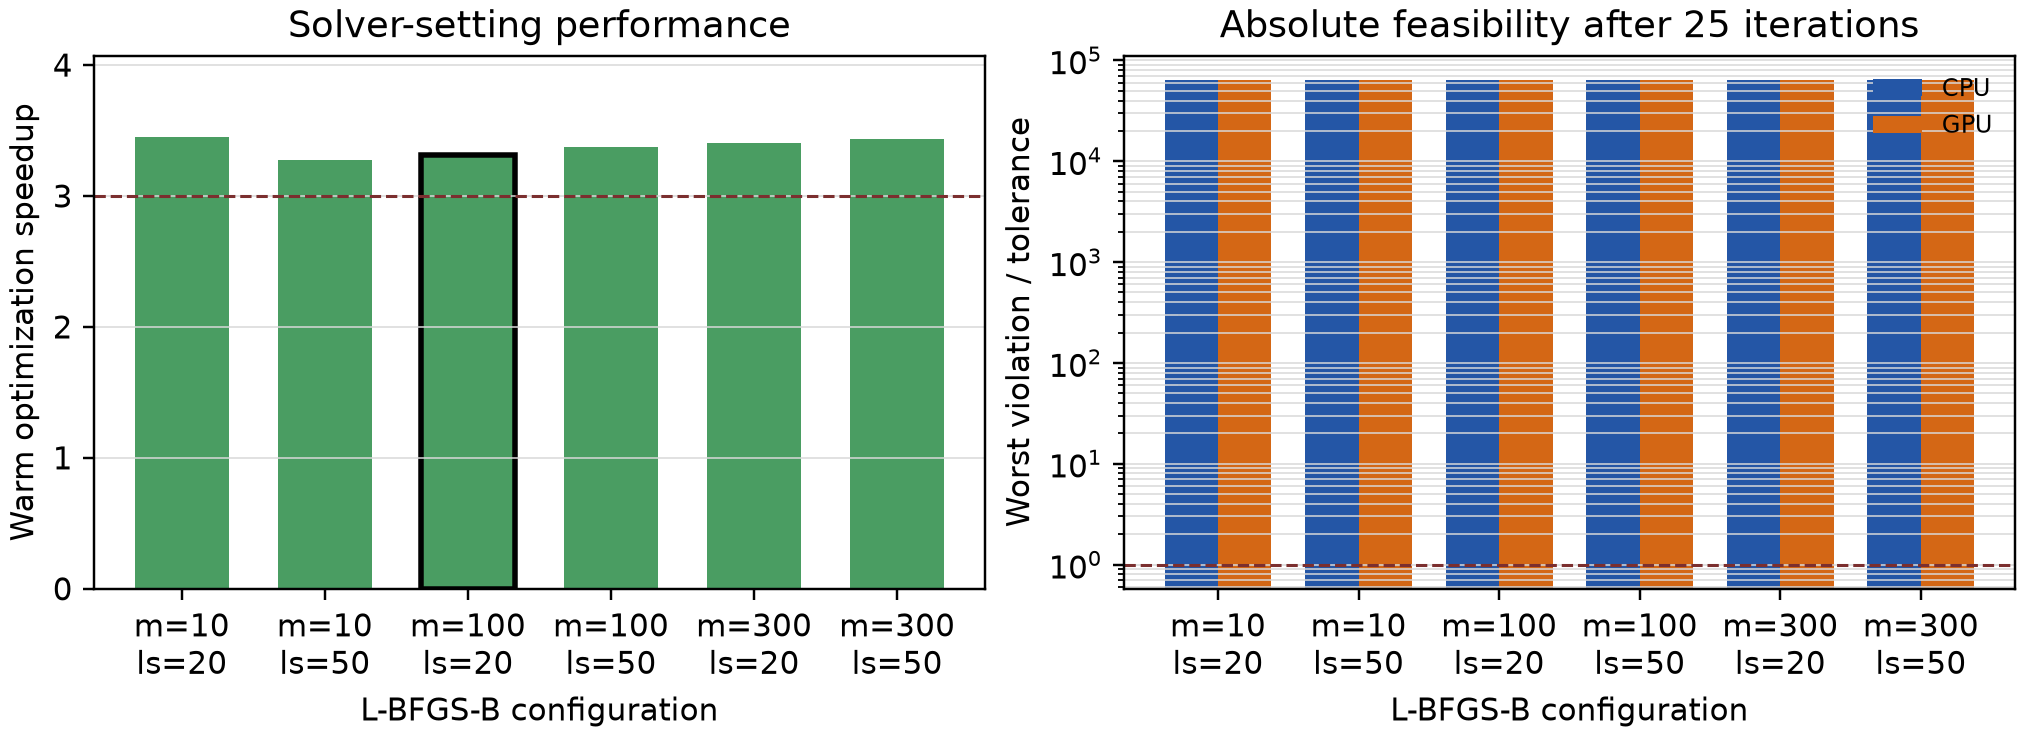
\includegraphics[width=\textwidth]{figures/feasibility_solver_sweep.png}
\caption{Tesla T4 solver-setting sweep.  The outlined bar is the deterministic
winner.  All configurations are fast, but the absolute constraints are still
orders of magnitude outside tolerance after only 25 iterations.}
\label{fig:feasibility-sweep}
\end{figure}

The selected setting then ran three synchronized stages.  GPU and CPU initial
objective discrepancies never exceeded $5.96\times10^{-19}$ and initial
gradient relative error never exceeded $7.09\times10^{-13}$.  Across each
25-iterate parity window, the maximum objective discrepancy was
$1.26\times10^{-10}$ and maximum curve-state relative error
$4.88\times10^{-8}$, so every backend gate passed even as the later nonconvex
paths separated.

{\scriptsize
\begin{center}
\begin{tabular}{rrrrrrl}
\toprule
Penalty & Iterations & Evaluations C/G & Seconds C/G & Speedup &
  Worst violation/tolerance C/G & Next seed \\
\midrule
$1\times$   & 100 & 140/152 & 150.35/45.68 & 3.291 & 4269.88/2604.92 & GPU \\
$10\times$  & 100 & 163/156 & 176.63/46.95 & 3.762 & 309.49/651.85 & CPU \\
$100\times$ & 200 & 430/493 & 460.05/151.02 & 3.046 & 61.61/21.64 & final \\
\bottomrule
\end{tabular}
\end{center}
}

In aggregate, CPU and GPU used 733 and 801 physics evaluations and took
787.035 and 243.653 seconds.  Warm speedup was $3.230\times$; including all
19.588 seconds of stage compilation gives $2.990\times$.  The GPU used 9.28\%
more evaluations overall.  The final stage alone used 14.65\% more and failed
its 10\% evaluation-budget gate, although it retained a $3.046\times$ wall-time
advantage.

\begin{figure}[htbp]
\centering
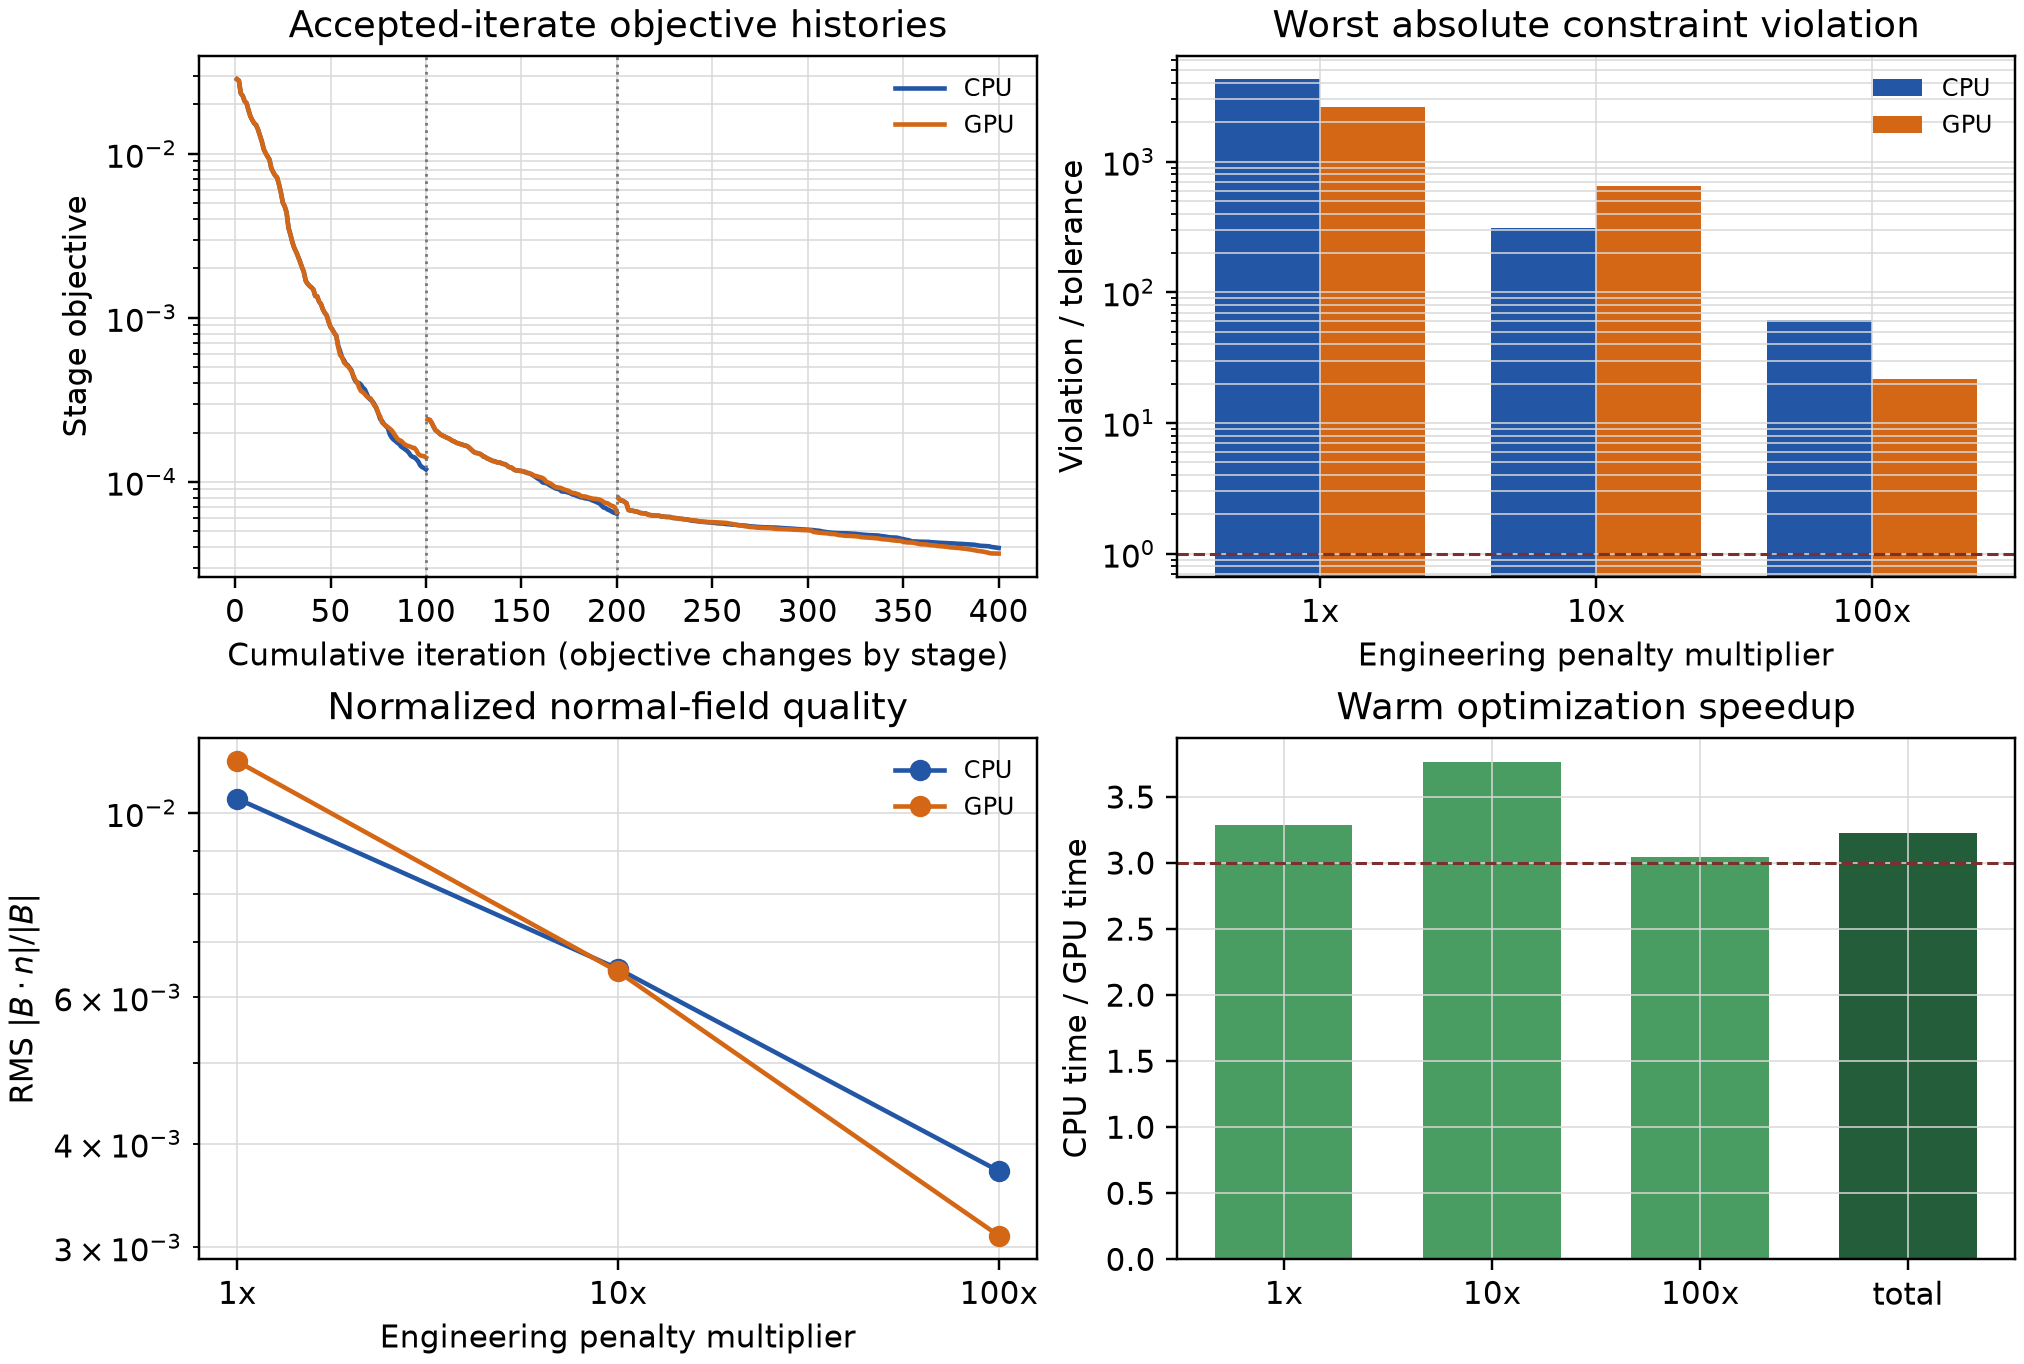
\includegraphics[width=\textwidth]{figures/feasibility_continuation.png}
\caption{Synchronized penalty continuation.  Vertical lines mark objective
changes and common restarts.  Larger weights greatly reduce violations, while
the GPU objective retains its production speed advantage.  The dashed lines
are the absolute-feasibility ratio one and speedup three gates.}
\label{fig:feasibility-continuation}
\end{figure}

Both final solves stopped at the 200-iteration cap rather than satisfying
SciPy's convergence condition.  Optimizer-coordinate gradient norms were
$1.675\times10^{-3}$ (CPU) and $6.270\times10^{-3}$ (GPU), far above the
$10^{-5}$ stationarity gate.  Nevertheless, the continuation moved the designs
substantially closer to the engineering limits:

\begin{center}
\begin{tabular}{lrrr}
\toprule
Final CPU-oracle metric & Limit & CPU & GPU \\
\midrule
Mean $|B\cdot n|/|B|$ & -- & 0.003054 & 0.002475 \\
RMS $|B\cdot n|/|B|$ & -- & 0.003707 & 0.003099 \\
Maximum $|B\cdot n|/|B|$ & -- & 0.009827 & 0.009542 \\
Minimum coil--coil distance & 0.100 & 0.100007 & 0.099994 \\
Minimum coil--surface distance & 0.300 & 0.299421 & 0.299465 \\
Maximum curvature & 5.000 & 4.913586 & 4.861377 \\
Maximum mean-squared curvature & 5.000 & 5.061614 & 5.021635 \\
Total base-coil length & -- & 29.255706 & 29.283627 \\
\bottomrule
\end{tabular}
\end{center}

Maximum curvature and coil--coil distance satisfy their absolute allowances on
both paths (the GPU's $6.32\,\mu$m coil--coil deficit is below the 0.1~mm
allowance).  The gate still correctly fails two constraints per backend.  The
coil--surface deficits are 0.579~mm (CPU) and 0.535~mm (GPU), or 5.79 and 5.35
times tolerance.  Mean-squared-curvature excesses are 0.0616 and 0.0216, or
61.6 and 21.6 times tolerance.  Thus ``close to the nominal limit'' is not
silently relabeled feasible.

The GPU final design improves mean, RMS, and maximum normalized normal field by
18.9\%, 16.4\%, and 2.9\% relative to the CPU continuation endpoint, so the
relative field-quality gate passes.  This is still a trade: the GPU RMS is
$3.38\times$ the unconverged 300-iteration $1\times$-weight result because the
stronger objective spends freedom on engineering constraints.  The final VTS
maps have signed correlation 0.926, relative $L^2$ difference 0.378, and lower
GPU absolute error at 65.7\% of surface points.

\begin{figure}[htbp]
\centering
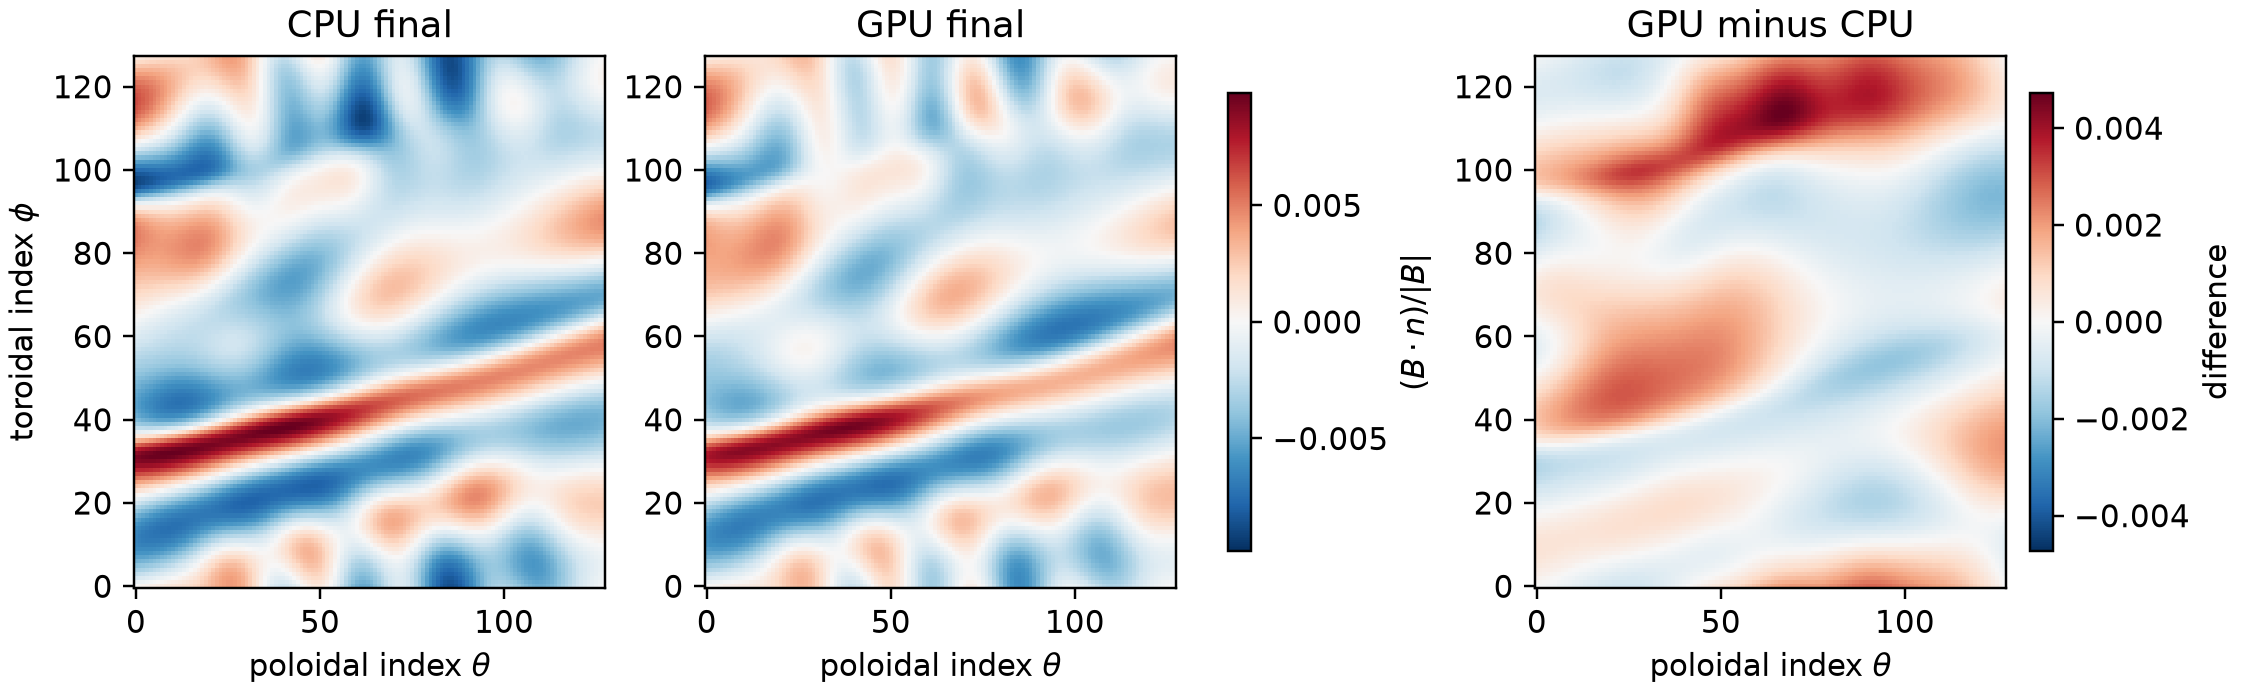
\includegraphics[width=\textwidth]{figures/feasibility_surface_field.png}
\caption{Final $100\times$-stage normalized normal-field maps from the archived
VTS files.  CPU and GPU panels share one scale; the difference uses its own
symmetric scale.}
\label{fig:feasibility-surface}
\end{figure}

\textbf{Decision.}  Accept the GPU objective's reproducibility, all staged
backend-parity checks, final visualization artifacts, and sustained warm
speedup.  Reject the milestone as stationary or absolutely engineering-
feasible.  Do not increase all penalty weights to $1000\times$: a finite
quadratic penalty admits residual constraint error and increasing it further
worsens conditioning while the current inner solves are already nonstationary.
The next implementation will expose named constraint quantities from the GPU
objective and add an augmented-Lagrangian outer loop while retaining SciPy for
the controlled inner solve.  The precise formulation is selected in the next
section.  Multipliers and penalty parameters must be stored per stage, and the
same absolute, parity, evaluation, field-quality, speed, and VTK contracts
remain in force.  A native L-BFGS solver remains deferred until that formulation
reaches a common feasible stationary solution.
\endgroup

\section{Equality-zero augmented Lagrangian implementation}
\label{sec:equality-al}

\subsection{Decision and mathematical contract}

The implemented method follows the augmented-Lagrangian convention in the
supplied \code{auglag\_qa.py} workflow, replacing the previously proposed
Powell--Hestenes--Rockafellar (PHR) projected-inequality formulation.  For a
base objective $f$, nonnegative zero-target constraints $c_i$, multipliers
$\lambda_i$, and componentwise penalties $\mu_i>0$, the inner problem is
\begin{equation}
  \mathcal L_A(x,\lambda,\mu)
  = f(x)-\lambda^T c(x)
    +\frac{1}{2}\sum_i\mu_i c_i(x)^2,
  \qquad
  \nabla_x\mathcal L_A
  = \nabla f + J_c^T(-\lambda+\mu\odot c).
  \label{eq:equality-zero-al}
\end{equation}
This sign convention requires the successful multiplier update
$\lambda\leftarrow\lambda-\mu\odot c$.  It is internally consistent but must
not be mixed with software that uses $f+\lambda^Tc$.  The initial multipliers
are deterministic zeros rather than the reference implementation's random
signed values, because reproducible CPU/GPU trajectories are part of the
validation contract.

The physics split is adapted rather than copied blindly.  Quadratic flux and
the small linear length regularizer remain the quantity to minimize,
\[
  f(x)=J_{\rm flux}(x)+10^{-6}\sum_k L_k(x),
\]
while the four engineering terms form $c$.  Each is an existing nonnegative
SIMSOPT hinge-penalty objective and is exactly zero when the corresponding
inequality is feasible.

\begin{center}
\begin{tabular}{lll}
\toprule
Constraint entry & Zero-level-set meaning & Stored physical check \\
\midrule
$c_{cc}$ & coil--coil distance penalty is zero & $d_{cc}^{\min}\geq0.1$ m \\
$c_{cs}$ & coil--surface distance penalty is zero & $d_{cs}^{\min}\geq0.3$ m \\
$c_{\kappa}$ & integrated curvature hinge is zero & $\max\kappa\leq5$ \\
$c_{\rm MSC}$ & squared MSC hinge is zero & $\max\langle\kappa^2\rangle\leq5$ \\
\bottomrule
\end{tabular}
\end{center}

This construction has an important consequence: the augmented term squares an
already quadratic hinge penalty.  It can therefore be fourth order in a raw
distance or curvature violation.  That behavior is intentional here because
it matches the supplied approach; it is also a conditioning risk to measure.
The acceptance decision continues to use the direct distances and curvatures,
not merely $\lVert c\rVert$, so a small integrated penalty cannot conceal a
localized physical violation.

\subsection{Execution structure}

\begin{figure}[htbp]
\centering
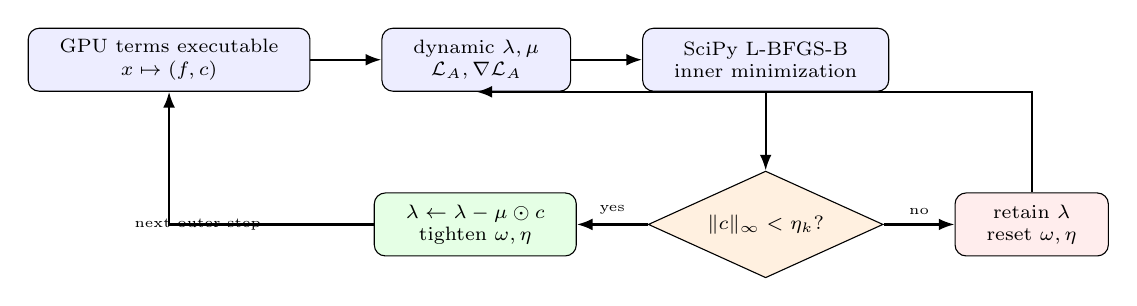
\begin{tikzpicture}[
  node distance=6mm and 9mm,
  box/.style={draw,rounded corners,align=center,minimum height=8mm,
              inner xsep=4mm,fill=blue!7,font=\scriptsize},
  decision/.style={draw,diamond,aspect=2.2,align=center,fill=orange!12,
                   font=\scriptsize,inner sep=1.5mm},
  flow/.style={-{Latex[length=2mm]},thick}
]
\node[box] (terms) {GPU terms executable\\$x\mapsto(f,c)$};
\node[box,right=of terms] (al) {dynamic $\lambda,\mu$\\$\mathcal L_A,\nabla\mathcal L_A$};
\node[box,right=of al] (inner) {SciPy L-BFGS-B\\inner minimization};
\node[decision,below=10mm of inner] (progress) {$\lVert c\rVert_\infty<\eta_k$?};
\node[box,left=of progress,fill=green!10] (lambda) {$\lambda\leftarrow\lambda-\mu\odot c$\\tighten $\omega,\eta$};
\node[box,right=of progress,fill=red!7] (penalty) {retain $\lambda$\\reset $\omega,\eta$};
\draw[flow] (terms) -- (al);
\draw[flow] (al) -- (inner);
\draw[flow] (inner) -- (progress);
\draw[flow] (progress) -- node[above,font=\tiny] {yes} (lambda);
\draw[flow] (progress) -- node[above,font=\tiny] {no} (penalty);
\draw[flow] (lambda.west) -| node[pos=0.25,left,font=\tiny]
  {next outer step} (terms.south);
\draw[flow] (penalty.north) |- (al.south);
\end{tikzpicture}
\caption{Implemented equality-zero augmented-Lagrangian loop.  Penalties grow
componentwise for nonzero constraints, and the same compiled JAX executable is
reused because $\lambda$ and $\mu$ are runtime inputs.}
\label{fig:equality-al-loop}
\end{figure}

The reusable \code{ScipyAugmentedLagrangianBridge} compiles both
$x\mapsto(f,c)$ and Equation~\eqref{eq:equality-zero-al}.  Multipliers and
penalties are executable arguments rather than closed-over Python constants,
so outer updates do not cause JAX recompilation.  The CPU oracle assembles the
same scalar and gradient from SIMSOPT partial derivatives in the exact
current-first coordinate order.  Each backend starts from the same physical
variables, zero multipliers, and common $\mu$, but then runs an independent
outer trajectory.  This tests the actual backend implementations rather than
forcing artificial lockstep updates.

The schema-5 artifact records every outer endpoint, all inner iteration and
physics-evaluation counts, $f$, $c$, $\lVert\nabla\mathcal L_A\rVert$,
$\lambda$, $\mu$, $\omega$, $\eta$, and physical variables.  It also retains
the complete CPU-oracle final normalized-normal-field and coil-constraint
metrics for both paths.  As before, each final surface is exported to VTS with
signed and absolute $(B\cdot n)/|B|$ data and each symmetry-expanded coil set
to VTU.

\subsection{Local verification and NVIDIA experiment}

Unit tests cover the AL scalar and analytic gradient, dynamic-state executable
reuse, convergence on a nonnegative zero-target constraint, validation of
penalty inputs, and equality of all four GPU constraint values with their
SIMSOPT CPU counterparts.  A one-outer-step local smoke run of the minimal
problem achieved initial base-objective absolute error zero, constraint relative
$L^2$ error $1.39\times10^{-16}$, and AL-gradient relative $L^2$ error
$6.47\times10^{-16}$.  CPU and JAX executed on the same host in this smoke
test, so its timing is deliberately not reported as GPU performance.

The new \code{colab\_augmented\_lagrangian.ipynb} runs the stress problem with
eight outer steps, at most 50 L-BFGS-B iterations per inner problem,
$\mu_0=10$, $\tau=10$, $\mu_{\max}=10^{12}$, and the previously selected
$1024\times4320$ tiling.  The decision gates remain: float64 initial parity,
direct engineering feasibility, stationarity, final field and constraint
quality, physics-evaluation budget, and at least $3\times$ warm optimization
speedup.

\subsection{Measured production result}

The returned archive has SHA-256 digest
\begin{center}
{\scriptsize\ttfamily
f495bca131bd38e0d1299bfae78da49de65f97332cc39d23b40975705de1832a}
\end{center}
and records revision \code{c7d522f6}.  It contains the schema-5 JSON and all
four required VTS/VTU files.  JAX selected \code{cuda:0}; the artifact did not
record the accelerator model, which is a provenance gap to repair in the next
runner revision.

Initial parity is substantially tighter than the gate: the base-objective and
augmented-Lagrangian absolute errors are both $1.39\times10^{-17}$, the
constraint vector agrees exactly, and the gradient relative $L^2$ error is
$1.53\times10^{-15}$.  This validates the GPU formulation at the common
starting state.  It does not imply matching final designs after long,
nonsmooth, independently executed L-BFGS-B trajectories.

\begin{figure}[htbp]
\centering
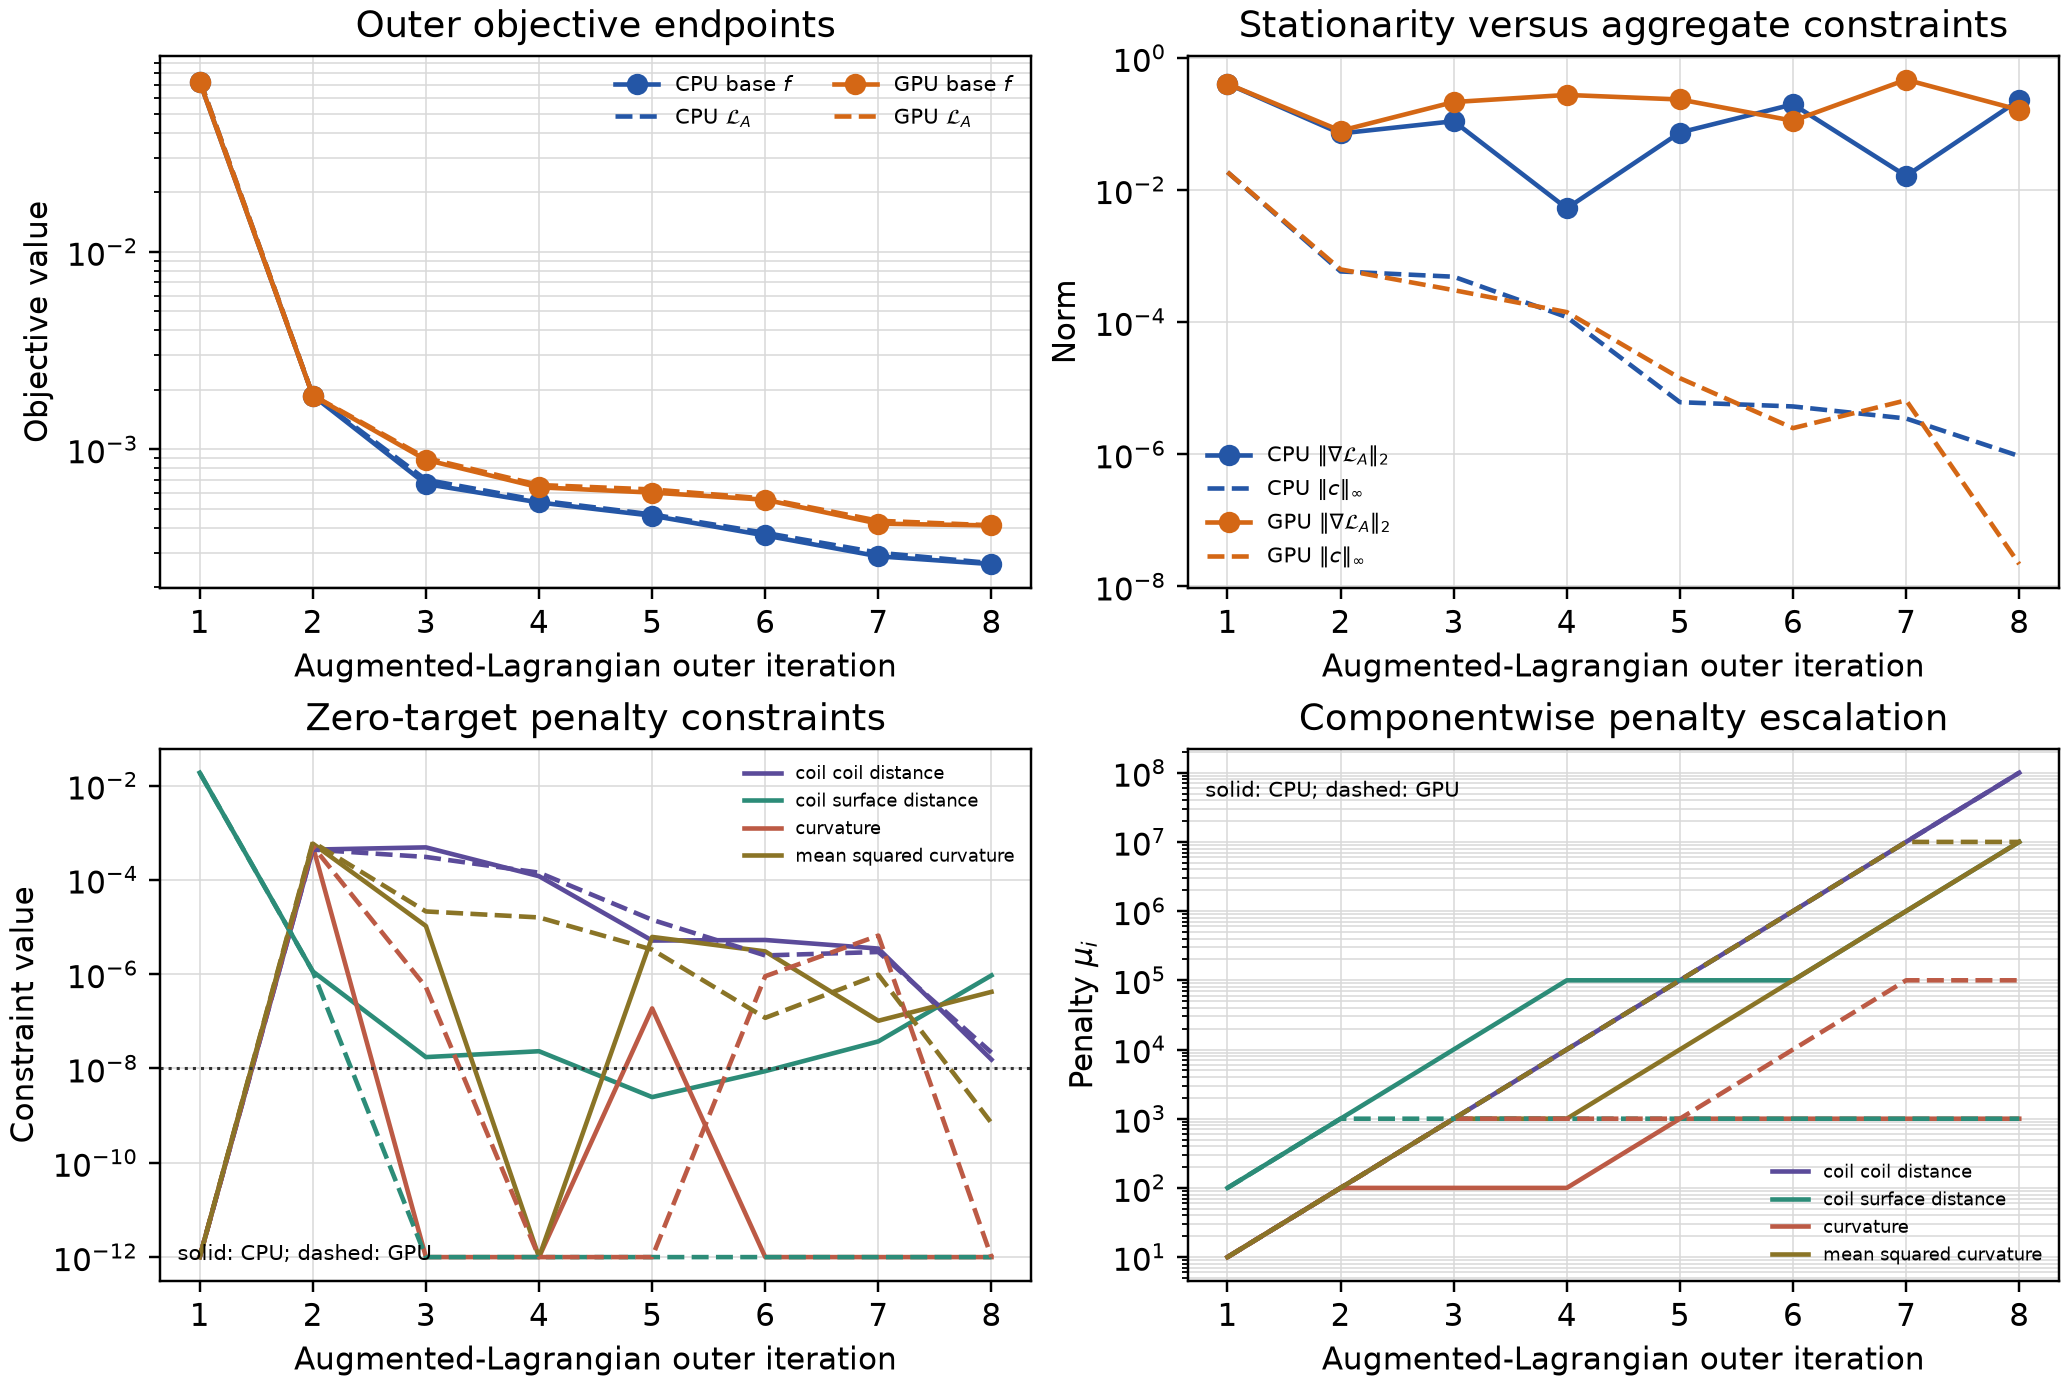
\includegraphics[width=\textwidth]{figures/augmented_lagrangian_convergence.png}
\caption{Production augmented-Lagrangian histories.  Aggregate constraint
values decrease while stationarity does not: every inner solve after the first
hits its 50-iteration cap, and componentwise penalties grow as high as
$10^8$.  A plotted value of $10^{-12}$ denotes an exactly zero constraint.}
\label{fig:augmented-lagrangian-convergence}
\end{figure}

The first inner solve accepts the starting point under its loose initial
projected-gradient tolerance.  Each of the remaining seven inner solves uses
all 50 iterations, giving 350 iterations in total per backend.  Neither path
approaches the requested stationarity: final
$\lVert\nabla\mathcal L_A\rVert_2$ is 0.2313 on CPU and 0.1635 on GPU.  The
aggregate infinity norms are $9.41\times10^{-7}$ and
$2.18\times10^{-8}$, respectively, and both exceed the $10^{-8}$ target.
Penalty escalation is therefore outrunning the ability of the inner solver to
minimize each changing subproblem.

\begin{figure}[htbp]
\centering
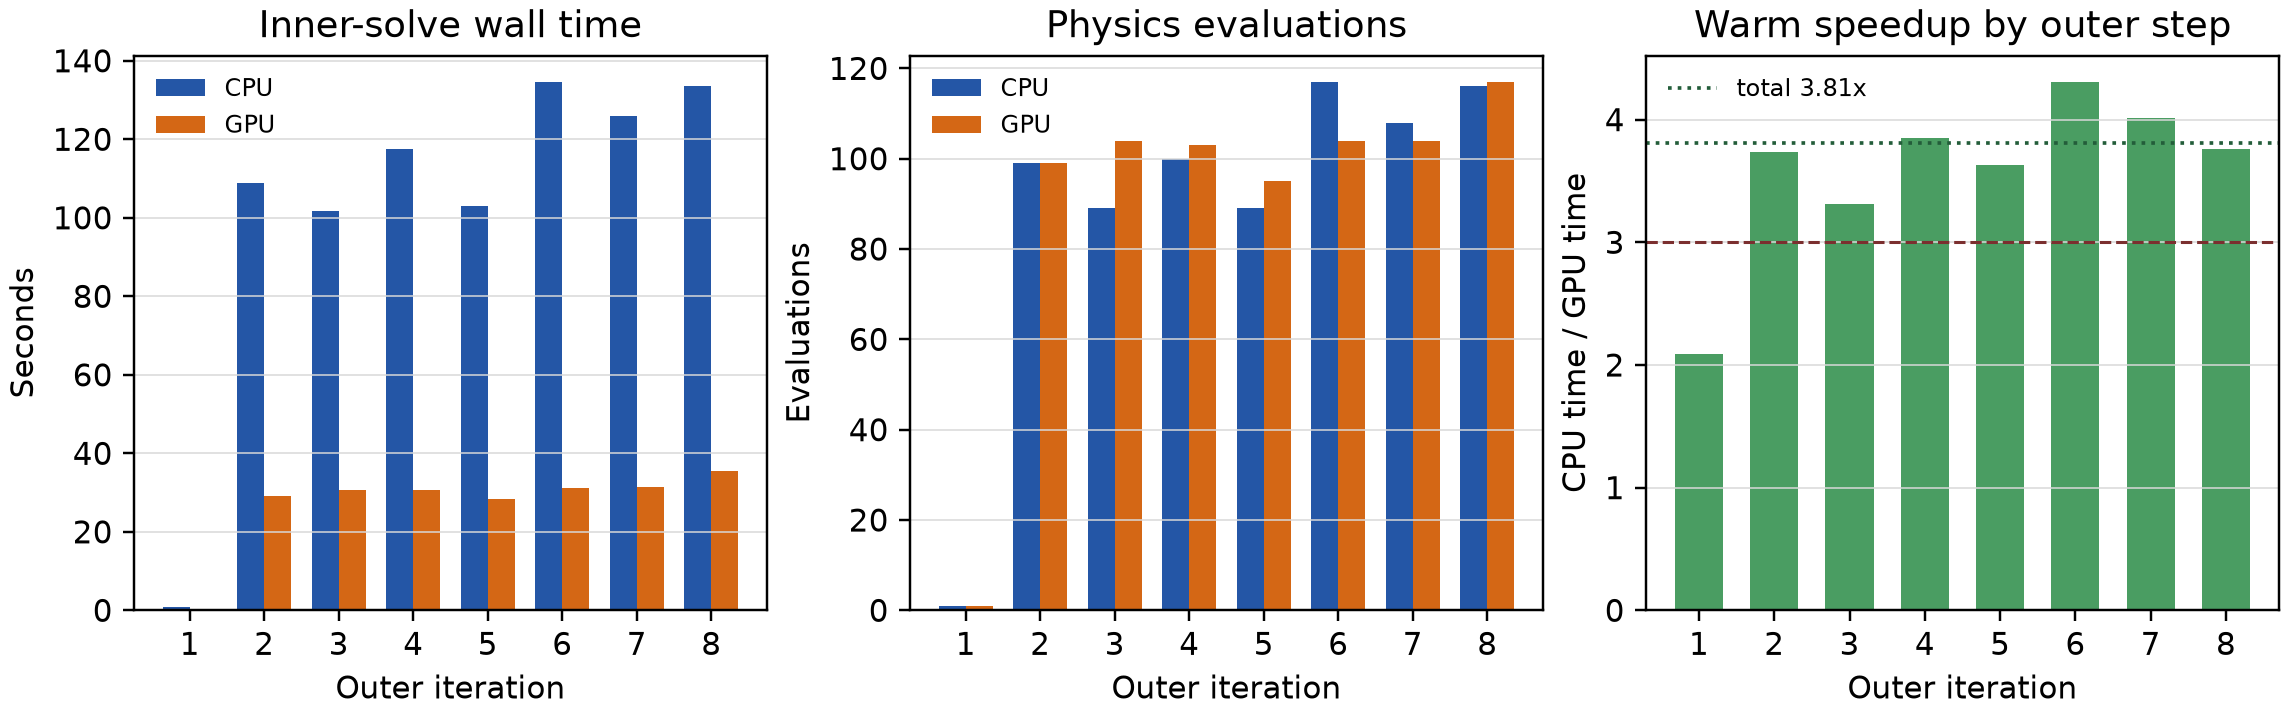
\includegraphics[width=\textwidth]{figures/augmented_lagrangian_performance.png}
\caption{Per-outer-step timing, physics-evaluation counts, and warm speedup.
The steady GPU advantage persists across the expensive inner solves while
evaluation counts remain comparable.}
\label{fig:augmented-lagrangian-performance}
\end{figure}

The CPU path takes 831.44~s and 719 physics evaluations; the GPU path takes
218.10~s and 727 evaluations.  Warm speedup is $3.812\times$.  Including the
8.22~s compilation cost gives $3.674\times$, so the performance and evaluation
budget gates pass.  Outer-step speedups range from $2.09\times$ for the trivial
first step to $4.31\times$; all seven substantive inner solves exceed
$3.3\times$.

\begin{center}
\begin{tabular}{lrrr}
\toprule
Final CPU-oracle metric & Limit & CPU AL & GPU AL \\
\midrule
Mean $|B\cdot n|/|B|$ & -- & 0.013136 & 0.017131 \\
RMS $|B\cdot n|/|B|$ & -- & 0.018998 & 0.024647 \\
Maximum $|B\cdot n|/|B|$ & -- & 0.083779 & 0.107443 \\
Minimum coil--coil distance (m) & 0.100 & 0.098842 & 0.098715 \\
Minimum coil--surface distance (m) & 0.300 & 0.285872 & 0.302344 \\
Maximum curvature & 5.000 & 4.943583 & 4.850320 \\
Maximum mean-squared curvature & 5.000 & 5.000844 & 5.000026 \\
Total base-coil length (m) & -- & 30.997526 & 30.854413 \\
\bottomrule
\end{tabular}
\end{center}

Direct metrics expose a weakness that the integrated constraint norm alone
cannot resolve.  The CPU coil--coil deficit is 1.158~mm and its coil--surface
deficit is 14.128~mm; both exceed the 0.1~mm allowance.  The GPU coil--coil
deficit is 1.285~mm, while its coil--surface distance is feasible by 2.344~mm.
Both paths satisfy maximum-curvature and allowed mean-squared-curvature excess.
Thus CPU fails two direct constraints and GPU fails one even though their
integrated penalty objectives have become small.  Squaring and integrating a
local hinge violation before treating it as a scalar equality permits a narrow
but physically important violation to contribute very little to $c$.

The GPU field result is also worse than the CPU endpoint: mean, RMS, and maximum
normalized normal field increase by 30.4\%, 29.7\%, and 28.2\%.  The final VTS
maps have signed correlation 0.984 and relative $L^2$ difference 0.369, but the
GPU has smaller pointwise absolute error on only 24.1\% of surface points.

\begin{figure}[htbp]
\centering
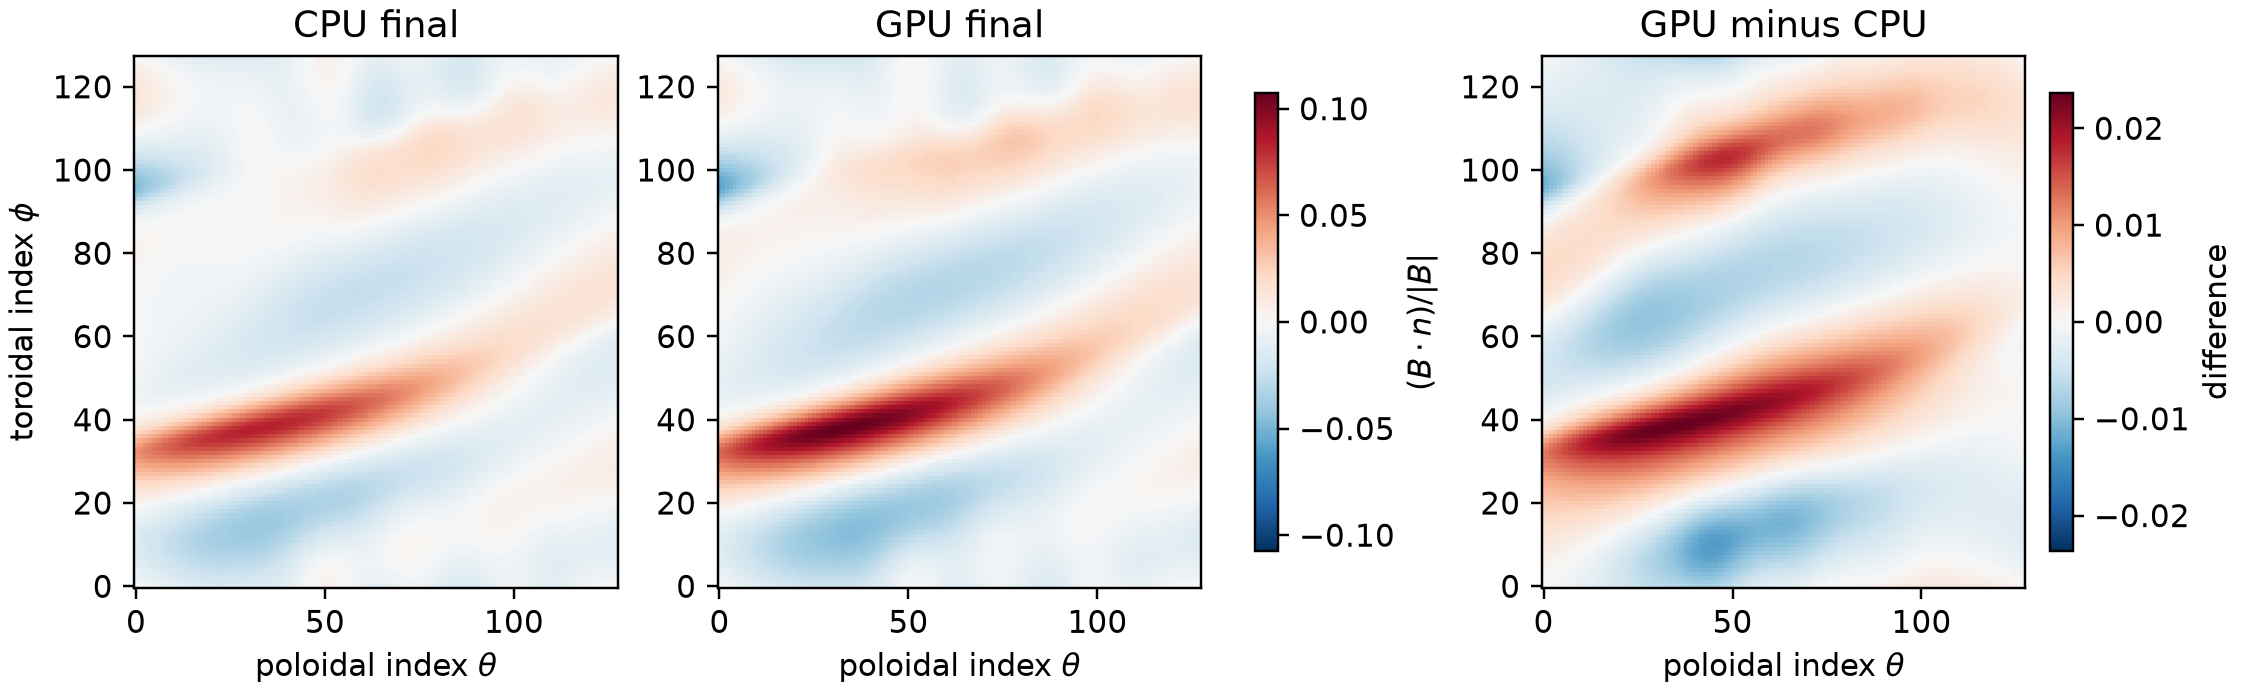
\includegraphics[width=\textwidth]{figures/augmented_lagrangian_surface_field.png}
\caption{Final normalized normal-field maps read directly from the archived
VTS files.  The GPU and CPU retain the same large-scale pattern but reach
meaningfully different endpoints after the AL trajectories bifurcate.}
\label{fig:augmented-lagrangian-surface}
\end{figure}

\textbf{Decision.}  Accept the GPU-native term implementation, float64 parity,
artifact completeness, evaluation budget, and sustained speedup.  Reject this
run as stationary, backend-equivalent at the final endpoint, or absolutely
engineering-feasible.  Do not merely add more outer iterations: penalties have
already reached $10^8$ while the inner gradients remain $O(10^{-1})$, so the
same schedule would further damage conditioning.  The next controlled step is
an inner-solve and scaling study at fixed AL semantics: increase the inner
budget, reduce penalty growth, cap $\mu$ earlier, and normalize the four
constraint families.  In parallel, design a less lossy constraint interface
that exposes localized distance and curvature residuals instead of only one
integrated squared penalty per family.  A formulation change must preserve the
user-selected equality-zero AL convention unless a separate comparison is
explicitly authorized.

\subsection{Implemented conditioning experiment}

The next runner makes the proposed conditioning study reproducible rather than
changing the production schedule by inspection.  For a positive scale $s_i$
for each constraint family, define
\begin{equation}
  \widehat c_i(x)=\frac{c_i(x)}{s_i},\qquad
  \mathcal L_A=f-\lambda^T\widehat c
    +\frac12\sum_i\mu_i\widehat c_i^2,
  \qquad
  \lambda\leftarrow\lambda-\mu\odot\widehat c.
  \label{eq:scaled-equality-zero-al}
\end{equation}
Scaling changes the conditioning of each AL subproblem, but it does not change
the feasibility contract.  The stopping test, componentwise penalty-growth
mask, and physical gates all use raw $c_i$ and direct distances and
curvatures.  Every outer record stores both $c$ and $\widehat c$; this prevents
a scale choice from silently redefining the $10^{-8}$ raw-constraint target.
CPU and GPU implement the same chain rule, including the $1/s_i$ factor in
$J_c^T(-\lambda+\mu\odot\widehat c)$.

The schema-6 benchmark also captures accelerator name, UUID, driver, and memory
through \code{nvidia-smi}.  It retains complete final CPU and GPU objective,
normalized-normal-field, engineering-constraint, raw/scaled AL, timing, and
physical-variable data.  Production confirmation still exports two VTS
surfaces carrying signed and absolute $(B\cdot n)/|B|$ and two VTU coil sets.

\begin{center}
\begin{tabular}{lrrrrl}
\toprule
Candidate & Outer & Inner & $\mu_0$ & $\tau$ & Scale vector $s$ \\
\midrule
Baseline & 6 & 50 & 10 & 10 & $(1,1,1,1)$ \\
Long inner & 6 & 150 & 10 & 10 & $(1,1,1,1)$ \\
Gentle growth & 8 & 150 & 4 & 2 & $(1,1,1,1)$ \\
Scaled gentle & 8 & 150 & 4 & 2 &
$(5\!\times\!10^{-4},2\!\times\!10^{-2},6\!\times\!10^{-4},7\!\times\!10^{-4})$ \\
\bottomrule
\end{tabular}
\end{center}
The nonunit scales are rounded per-family maxima observed in the archived
production history, so a representative active value is order unity.  They
are an explicitly labelled data-derived candidate, not universal defaults.
The candidates isolate inner budget, penalty growth/cap, and family scaling as
far as a four-run screen permits.  The baseline and long-inner schedules cap
$\mu$ at $10^{12}$; gentle and scaled-gentle both cap it at $10^6$.  Thus the
last pair differs only in $s$, making scaling an identifiable intervention.

\begin{figure}[htbp]
\centering
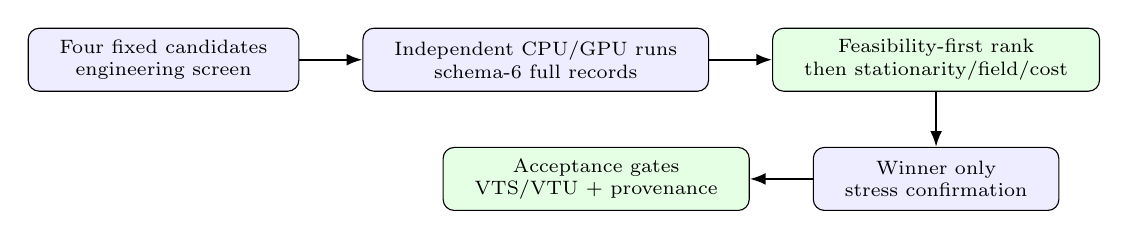
\begin{tikzpicture}[
  node distance=7mm and 8mm,
  box/.style={draw,rounded corners,align=center,minimum height=8mm,
              inner xsep=4mm,fill=blue!7,font=\scriptsize},
  gate/.style={draw,rounded corners,align=center,minimum height=8mm,
               inner xsep=4mm,fill=green!10,font=\scriptsize},
  flow/.style={-{Latex[length=2mm]},thick}
]
\node[box] (candidates) {Four fixed candidates\\engineering screen};
\node[box,right=of candidates] (records) {Independent CPU/GPU runs\\schema-6 full records};
\node[gate,right=of records] (rank) {Feasibility-first rank\\then stationarity/field/cost};
\node[box,below=of rank] (stress) {Winner only\\stress confirmation};
\node[gate,left=of stress] (artifacts) {Acceptance gates\\VTS/VTU + provenance};
\draw[flow] (candidates) -- (records);
\draw[flow] (records) -- (rank);
\draw[flow] (rank) -- (stress);
\draw[flow] (stress) -- (artifacts);
\end{tikzpicture}
\caption{Automated AL-conditioning workflow.  Screening is deliberately
performed on the smaller engineering case; only the feasibility-first winner
consumes a production-scale stress run and produces visualization artifacts.}
\label{fig:al-conditioning-workflow}
\end{figure}

Ranking is lexicographic: number of failed direct physical constraints,
largest and summed tolerance-normalized physical violation, number of
nonstationary backends, maximum final AL-gradient norm, mean CPU/GPU normalized
field RMS, then total physics evaluations.  A backend or initial-parity failure
makes a candidate ineligible.  Speed cannot compensate for a worse rank in
these quantities.  However, this first policy has no hard feasibility cutoff:
a candidate failing fewer checks can outrank one with much smaller violation
magnitudes.  The reduced screen selects a diagnostic candidate; it is not
itself evidence that the same ordering transfers to production scale.

The new \code{colab\_augmented\_lagrangian\_conditioning.ipynb} runs all GPU
tests, performs the four engineering screens, reruns the winner on the stress
problem, validates schema and required final metrics, checks all four VTK
artifacts, and downloads one archive.  No NVIDIA performance or quality result
is claimed yet: figures and the decision will be extended from the returned
archive, preserving the distinction between implemented experiment and
measured outcome.

\subsection{Measured conditioning-study result}

The returned archive has SHA-256 digest
\begin{center}
{\scriptsize\ttfamily
6298b735d451df4edfbe4c7e1ab8917fc2e24a64fd591498a7fcd87edd7ecc48}
\end{center}
and records revision \code{236461f6}.  The analyzer validated all ten members,
reproduced every candidate rank, checked every raw and scaled history, and
verified the signed and absolute surface arrays.  The run used a 15,360~MiB
Tesla T4 with driver 580.82.07; JAX selected \code{cuda:0}.  Production initial
parity remains excellent: base and AL absolute errors are
$1.39\times10^{-17}$ and $2.22\times10^{-16}$, the raw and scaled constraints
agree exactly, and gradient relative error is $4.80\times10^{-16}$.

\begin{figure}[htbp]
\centering
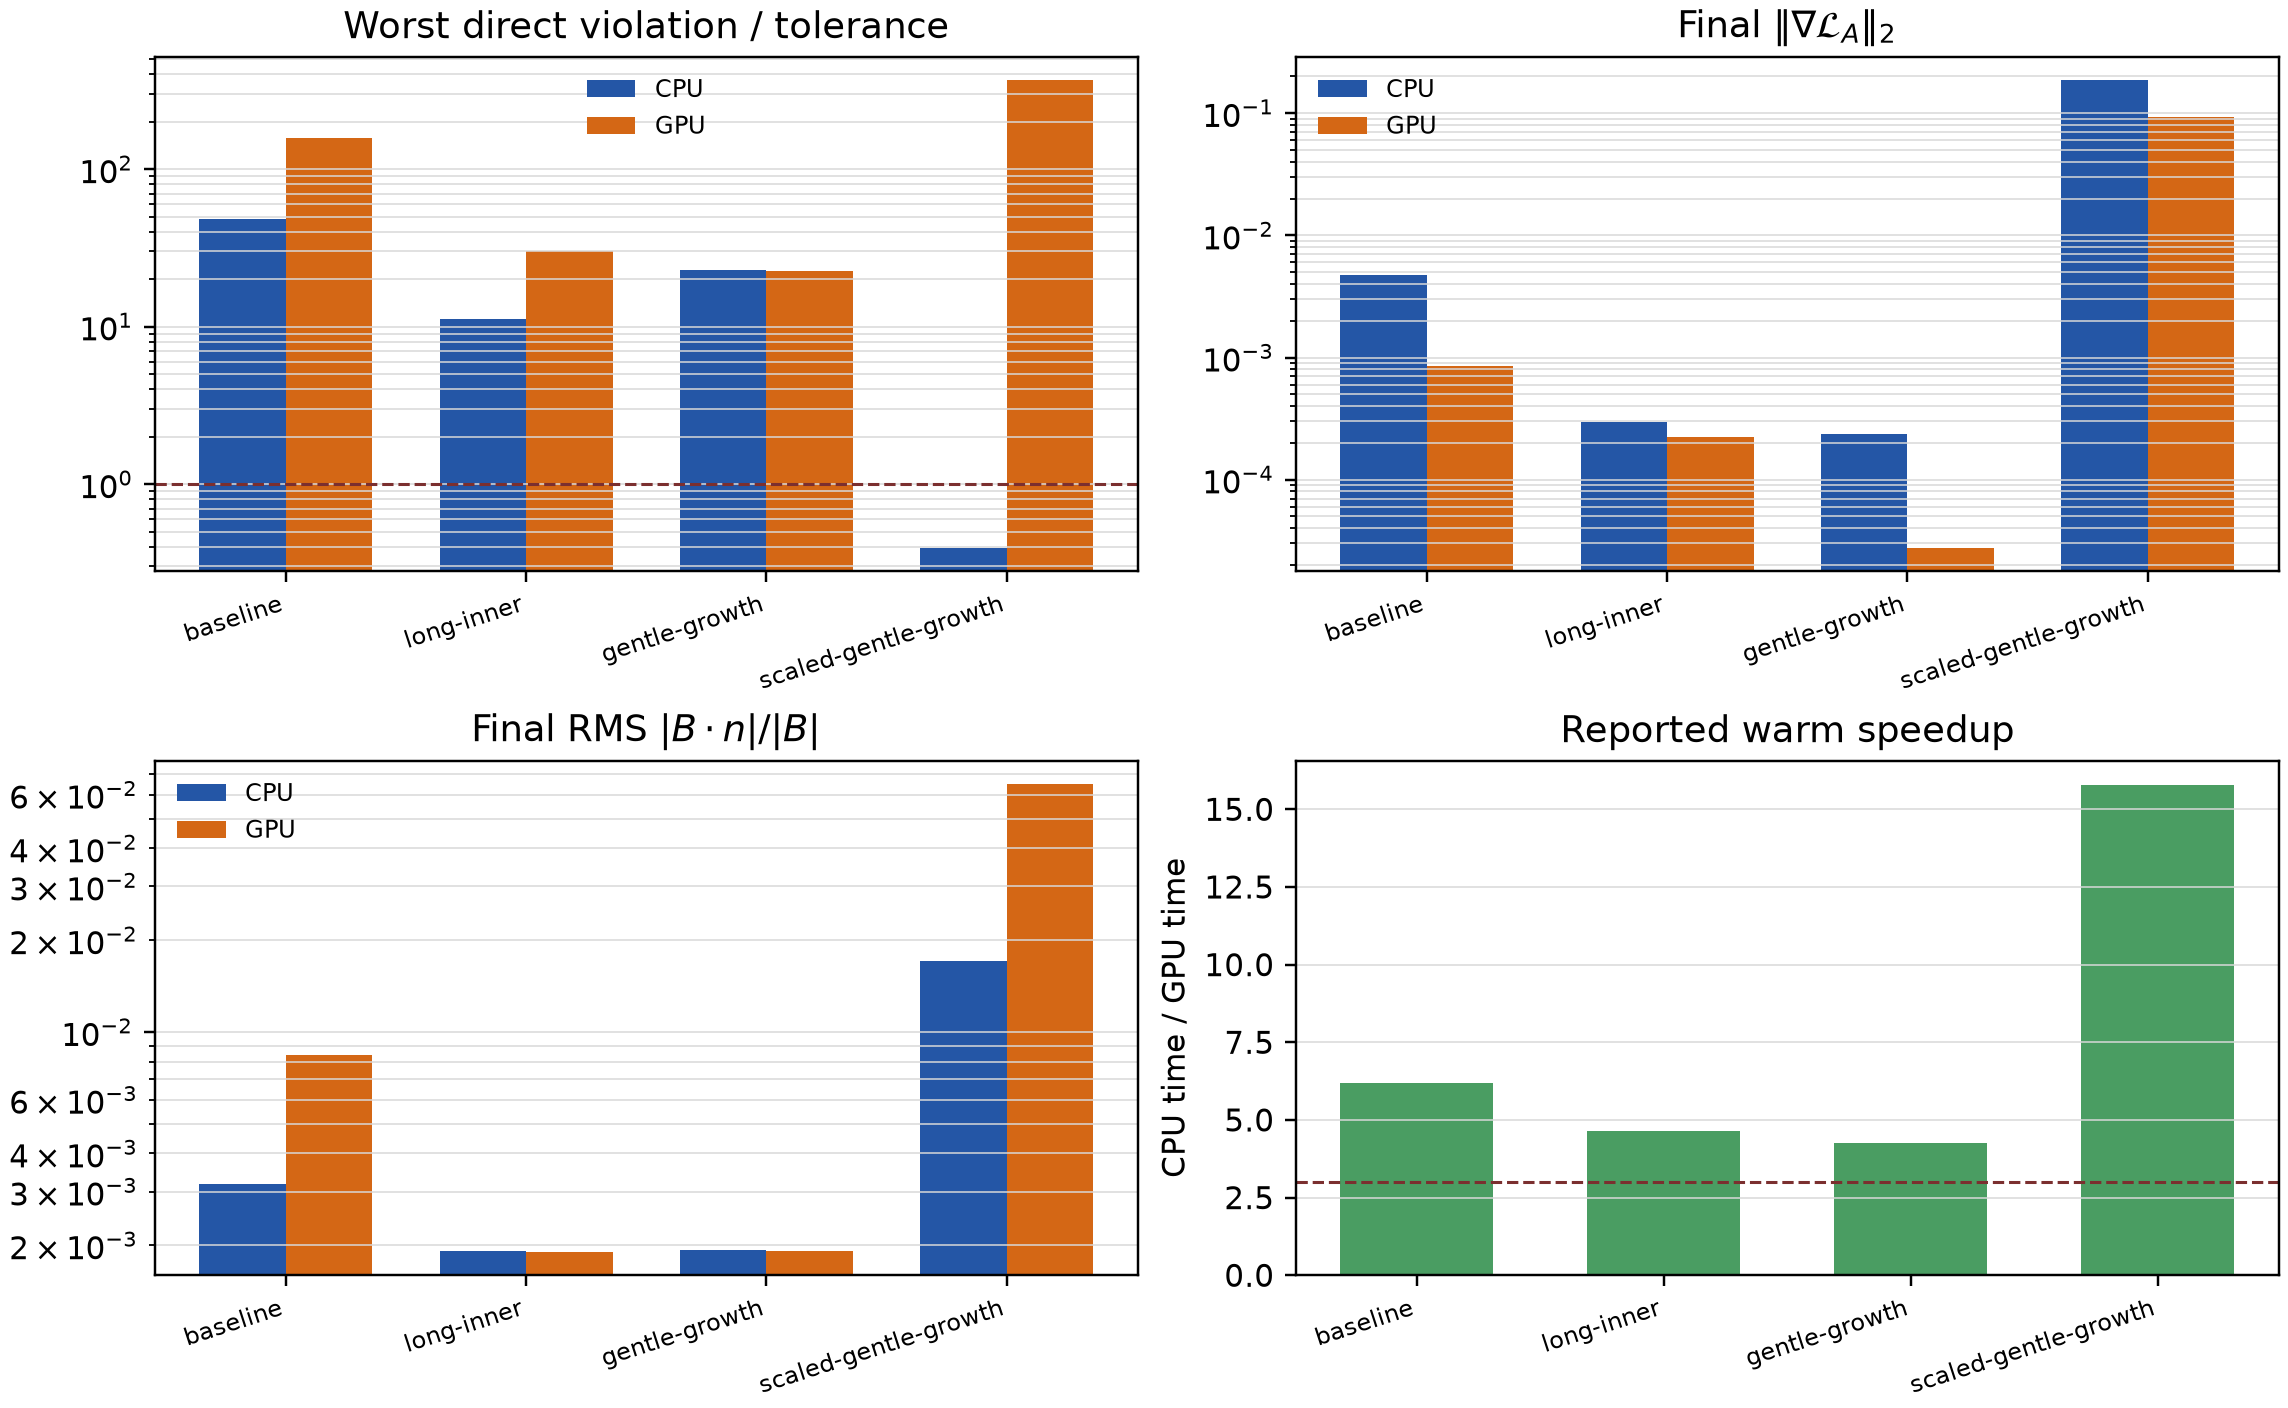
\includegraphics[width=\textwidth]{figures/al_conditioning_screen.png}
\caption{Engineering screening results.  None of the four candidates is both
physically feasible and stationary.  The conspicuous speedup of the scaled
case accompanies much less GPU work and a severely degraded endpoint, so it is
not evidence of faster equivalent optimization.}
\label{fig:al-conditioning-screen}
\end{figure}

\begin{center}
\scriptsize
\begin{tabular}{lrrrrrrr}
\toprule
Candidate & Failed checks & Worst ratio & CPU grad. & GPU grad. & CPU RMS & GPU RMS & Speedup \\
\midrule
Baseline & 2 & 156.54 & $4.69\!\times\!10^{-3}$ & $8.60\!\times\!10^{-4}$ & 0.00318 & 0.00841 & 6.19 \\
Long inner & 3 & 30.18 & $2.99\!\times\!10^{-4}$ & $2.22\!\times\!10^{-4}$ & 0.00192 & 0.00190 & 4.63 \\
Gentle growth & 3 & 22.88 & $2.38\!\times\!10^{-4}$ & $2.76\!\times\!10^{-5}$ & 0.00193 & 0.00191 & 4.27 \\
Scaled gentle & 1 & 368.66 & 0.188 & 0.0937 & 0.0171 & 0.0650 & 15.78 \\
\bottomrule
\end{tabular}
\end{center}

``Failed checks'' counts CPU and GPU direct constraints separately, and the
worst ratio divides a physical violation by its acceptance tolerance.  The
unscaled long-inner and gentle-growth candidates give the best field and
stationarity results, but each misses several tight physical tolerances.  The
scaled CPU endpoint satisfies all four physical allowances, whereas its GPU
endpoint misses only coil--surface distance---but by 36.866~mm, or
$368.66$ times the 0.1~mm allowance.  Because the first ranking key is the
number of failures, scaled-gentle mechanically outranks the baseline's two
failures despite having the worst violation magnitude and field quality.  This
is a selection-policy failure: when no candidate passes all hard gates, the
workflow should report ``no qualified winner'' instead of launching a nominal
winner as though it were acceptable.

The stress rerun is useful as a failure diagnostic.  CPU and GPU agree through
the first outer endpoint and remain close through the second.  At GPU outer
step three, L-BFGS-B consumes all 150 iterations and ends with
$\lVert\nabla\mathcal L_A\rVert_2=2.27$.  At each of steps four through eight,
it then returns after one iteration due to relative function reduction while
the optimizer vector is bitwise unchanged.  Penalties nevertheless grow to
$1024$, and the reported gradient rises monotonically to 131.36.  CPU continues
to move in four later stages but also finishes nonstationary with gradient
0.993.  Thus SciPy's inner \code{success} flag is not a sufficient AL-stage
acceptance condition; relative function stagnation with a large gradient must
be treated as failure, not progress.

\begin{figure}[htbp]
\centering
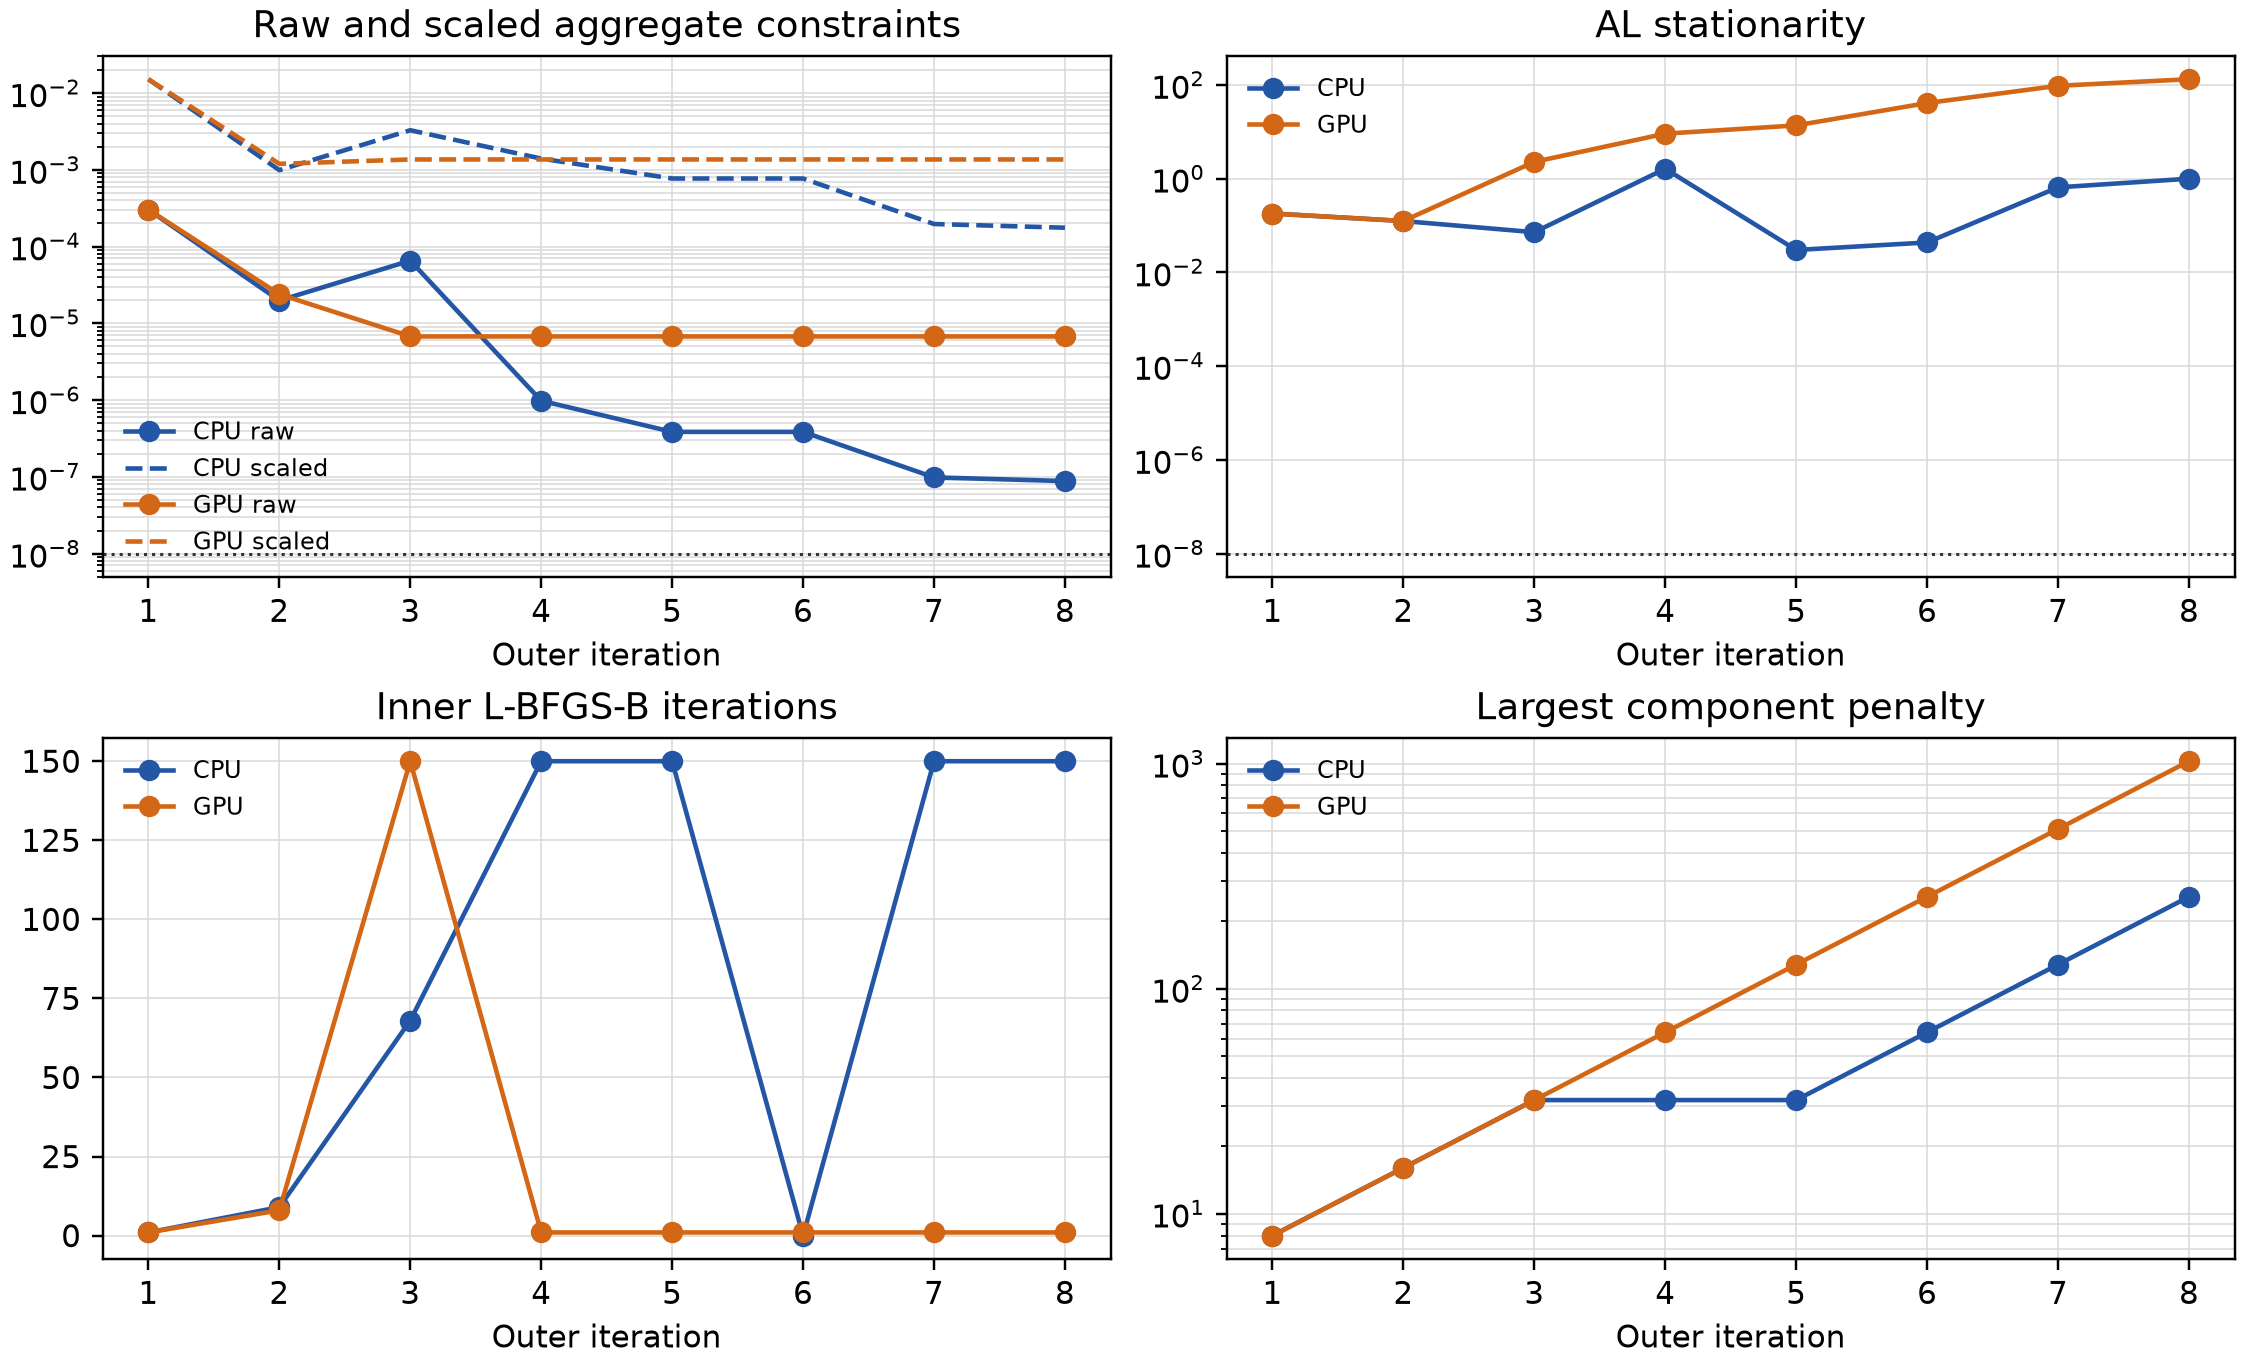
\includegraphics[width=\textwidth]{figures/al_conditioning_winner_convergence.png}
\caption{Stress trajectory of the mechanically selected scaled candidate.
After outer step three the GPU variables no longer move, while multipliers and
penalties continue changing and the AL gradient explodes.  Raw aggregate
constraints remaining small do not imply direct physical feasibility.}
\label{fig:al-conditioning-winner-convergence}
\end{figure}

The CPU path takes 1410.19~s, 678 inner iterations, and 1350 physics
evaluations.  GPU takes 99.69~s, 164 iterations, and 334 evaluations; compilation
adds 7.48~s.  The nominal warm and amortized ratios are $14.15\times$ and
$13.16\times$, but these compare unequal work and are rejected as optimization
speedups.  Normalizing only by recorded physics evaluations gives a more
defensible, though still trajectory-dependent, throughput indication of
$3.50\times$ (1.045 versus 0.298 seconds per evaluation).  This is consistent
with earlier objective speedups and does not rescue the failed solve.

\begin{center}
\begin{tabular}{lrrr}
\toprule
Production metric & Limit & CPU & GPU \\
\midrule
Final recorded objective & -- & $6.579\!\times\!10^{-4}$ & $2.815\!\times\!10^{-3}$ \\
Mean $|B\cdot n|/|B|$ & -- & 0.02263 & 0.04790 \\
RMS $|B\cdot n|/|B|$ & -- & 0.02740 & 0.06107 \\
Maximum $|B\cdot n|/|B|$ & -- & 0.08081 & 0.19623 \\
Minimum coil--coil distance (m) & 0.100 & 0.09572 & 0.09542 \\
Minimum coil--surface distance (m) & 0.300 & 0.30801 & 0.26978 \\
Maximum curvature & 5.000 & 4.46624 & 4.23661 \\
Maximum mean-squared curvature & 5.000 & 5.00022 & 5.00106 \\
\bottomrule
\end{tabular}
\end{center}

CPU misses coil--coil distance by 4.277~mm but passes the stated allowances for
the other direct constraints.  GPU misses coil--coil by 4.576~mm,
coil--surface by 30.219~mm, and mean-squared curvature by 0.001059 (slightly
beyond its 0.001 allowance).  GPU normalized-field mean, RMS, and maximum are
$2.12\times$, $2.23\times$, and $2.43\times$ the CPU values.  The final VTS
maps have signed correlation 0.820, relative $L^2$ difference 1.522, and GPU
has smaller pointwise absolute error on only 19.9\% of surface points.

\begin{figure}[htbp]
\centering
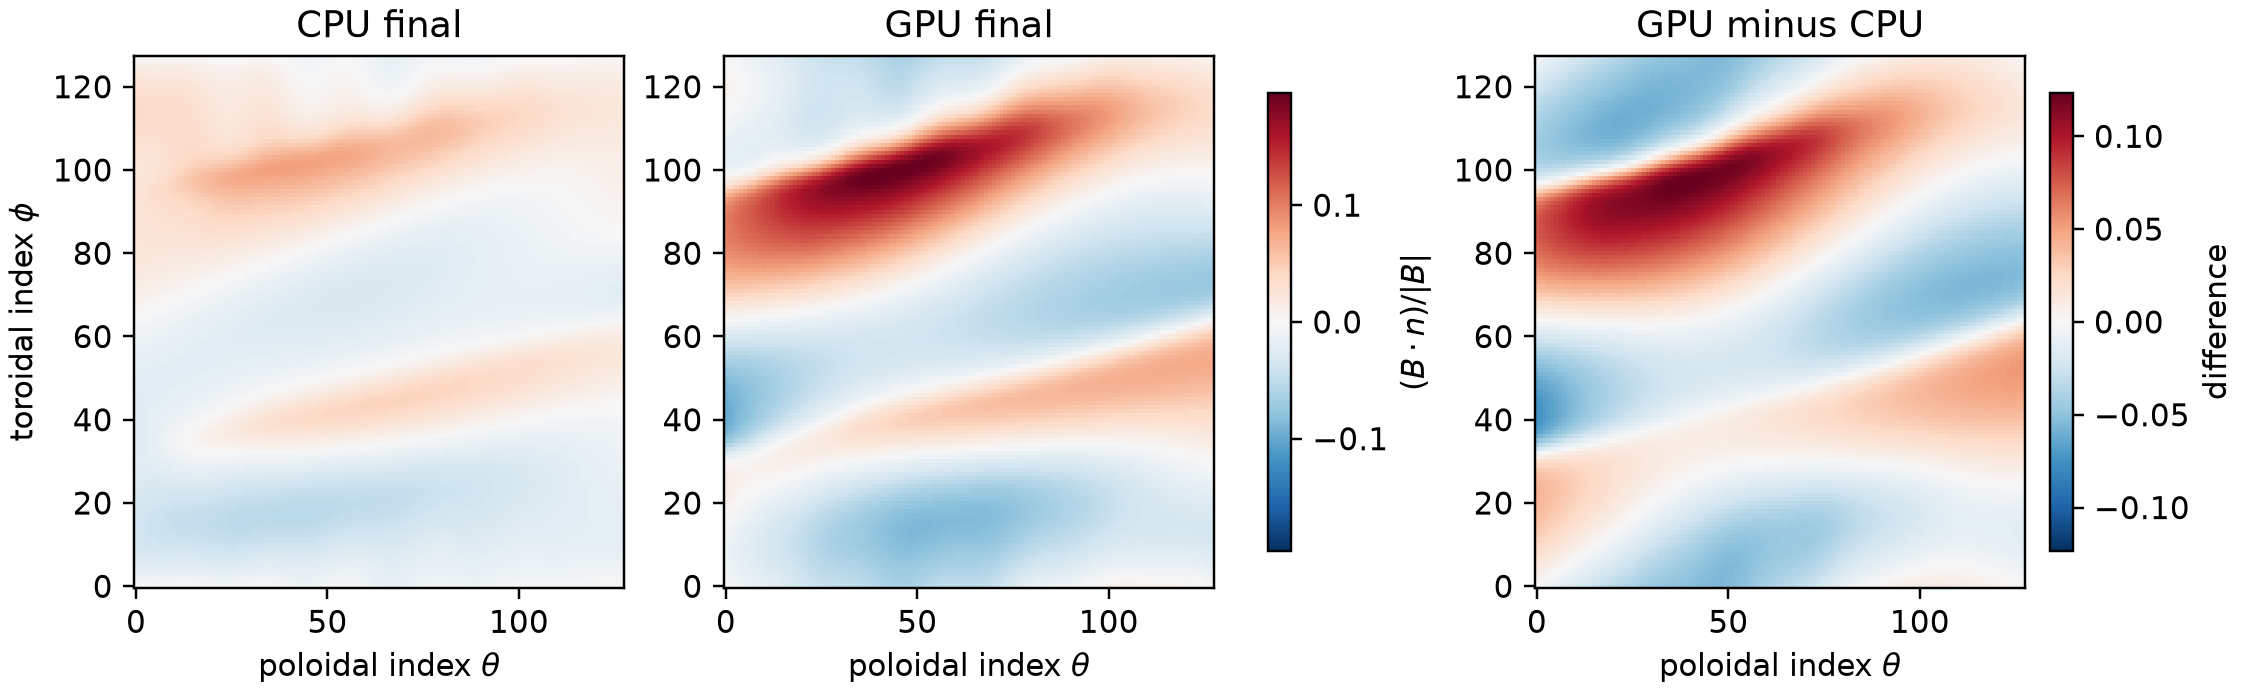
\includegraphics[width=\textwidth]{figures/al_conditioning_winner_surface_field.png}
\caption{Final normalized normal field from the archived VTS files.  The
stagnated GPU path has much larger coherent error bands and is not an
equivalent endpoint to the CPU trajectory.}
\label{fig:al-conditioning-winner-surface}
\end{figure}

\textbf{Decision.}  Accept the schema-6 raw/scaled accounting, CPU/GPU initial
parity, NVIDIA provenance, analyzer, and VTK exports.  Reject the tested
value-normalization scales, the mechanical winner, every final design, and the
whole-run speedup claim.  The result shows why making the already squared,
integrated hinge values order unity is not sound preconditioning: it introduces
effective quadratic penalty factors proportional to $1/s_i^2$ without
balancing the constraint Jacobians.  The next implementation must (i) require
hard feasibility and stationarity before declaring a winner, (ii) reject an
inner stage that stagnates with a large gradient and stop penalty escalation,
and (iii) derive conditioning from gradient/Jacobian norms or expose local
unsquared residuals.  Another blind scale or penalty sweep is not justified.

\subsection{Implemented safeguard and gradient-aware redesign}

The next implementation enforces those three decisions in schema~7.  First,
the outer loop records the requested inner tolerance, final infinity-norm
gradient, step norm, and whether the stage was accepted.  In strict mode an
inner solve is accepted only if
\[
  \|\nabla_x \mathcal L_A\|_\infty
  \leq \kappa\max(\omega_k,\epsilon_g),\qquad \kappa\geq 1.
\]
Failure terminates the run before either $\lambda$ or $\mu$ changes.  This
directly prevents the false-convergence sequence seen on the T4, where
L-BFGS-B stopped by relative function reduction while the gradient grew and
the outer loop continued increasing the penalty.

Second, the AL may use a zero-preserving, residual-like coordinate
\[
 q_\varepsilon(c)=\sqrt{c+\varepsilon^2}-\varepsilon,
 \qquad \widehat c_i=\frac{q_\varepsilon(c_i)}{s_i}.
\]
For the current nonnegative, integrated squared-hinge objectives this mapping
is exactly zero at feasibility and approaches $\sqrt c$ away from its smooth
region.  Therefore the AL quadratic behaves approximately quadratically in an
aggregate violation amplitude rather than quartically.  This is not identical
to exposing every local unsquared residual; it is a safe intermediate test that
does not change SIMSOPT's physical feasibility definition.

Third, automatic scaling is based on derivatives in the actual optimizer
coordinates.  At the initial state, with zero multipliers, the estimated norm
of constraint family $i$'s penalty-gradient contribution is
\[
 A_i=\mu_0|q(c_i)|\,|q'(c_i)|\,\|\nabla_xc_i\|_2.
\]
For a requested maximum fraction $\rho$ of the base-objective gradient, the
applied attenuation is
\[
 s_i=\sqrt{\max\!\left(\frac{A_i}
 {\rho\max(\|\nabla f\|_2,\mathrm{tiny})},1\right)}.
\]
Because $s_i\geq1$, automatic calibration can only attenuate a family.  It can
never reproduce the previous $s_i<1$ amplification, while the archive records
the base gradient, every Jacobian row norm, unscaled estimate, recommended
scale, applied scale, and post-scaling estimate.

\begin{figure}[htbp]
\centering
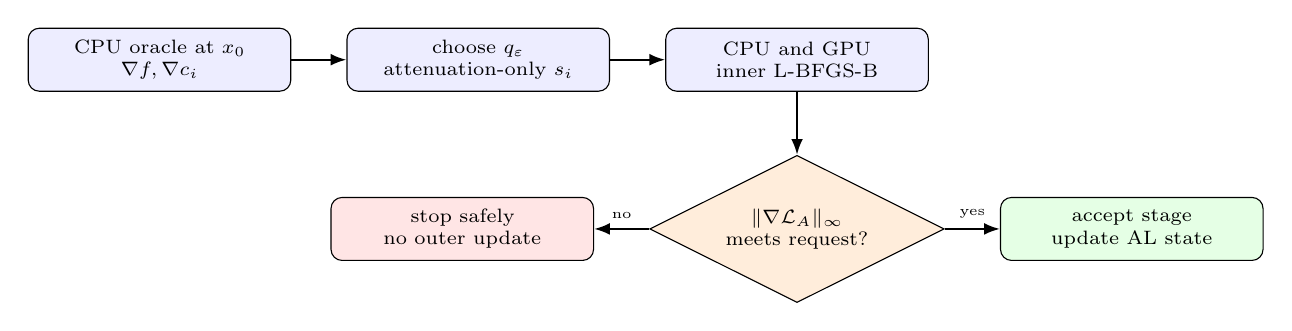
\begin{tikzpicture}[
  node distance=5mm and 7mm,
  box/.style={draw,rounded corners,align=center,minimum height=8mm,
              text width=31mm,fill=blue!7,font=\scriptsize},
  gate/.style={draw,diamond,aspect=2.0,align=center,fill=orange!14,
               font=\scriptsize,inner sep=1.5mm},
  flow/.style={-{Latex[length=2mm]},thick}
]
\node[box] (jac) {CPU oracle at $x_0$\\$\nabla f,\nabla c_i$};
\node[box,right=of jac] (map) {choose $q_\varepsilon$\\attenuation-only $s_i$};
\node[box,right=of map] (inner) {CPU and GPU\\inner L-BFGS-B};
\node[gate,below=8mm of inner] (stationary) {$\|\nabla\mathcal L_A\|_\infty$\\meets request?};
\node[box,left=of stationary,fill=red!10] (stop) {stop safely\\no outer update};
\node[box,right=of stationary,fill=green!10] (update) {accept stage\\update AL state};
\draw[flow] (jac) -- (map);
\draw[flow] (map) -- (inner);
\draw[flow] (inner) -- (stationary);
\draw[flow] (stationary) -- node[above,font=\tiny] {no} (stop);
\draw[flow] (stationary) -- node[above,font=\tiny] {yes} (update);
\end{tikzpicture}
\caption{Safeguarded AL stage.  Conditioning is calibrated once from physical
derivatives, while every outer update is conditional on measured inner
stationarity.}
\label{fig:al-safeguard-stage}
\end{figure}

The automated qualification screen contains an identity reference and three
smooth-square-root variants that isolate the smoothing width and maximum
initial gradient ratio.  All share the gentler $\mu_0=4$, $\tau=2$ schedule
and a 200-iteration inner budget.  Every CPU and GPU endpoint exports a coil
VTU and a surface VTS with signed and absolute $(B\cdot n)/|B|$ arrays.

Promotion is now a hard predicate rather than a ranking side effect.  A
candidate must pass GPU-backend provenance, float64 initial parity, direct
physical feasibility, stationary convergence, final normal-field quality, and
final constraint quality.  Only qualified candidates may be ranked for the
production stress run.  If none qualify, the summary reports no winner and
skips production; a diagnostic ordering remains available solely to guide the
next design.  Thus the new code makes a stronger methodological result before
new NVIDIA data exist: an invalid design can no longer become a production
\emph{winner}.  The NVIDIA outcome is reported below.
The companion analyzer independently reproduces every qualification and
diagnostic rank, rejects missing or inconsistent schema-7 stage fields,
validates all VTK payloads and signed/absolute surface arrays, and creates four
figures covering qualification, gradient calibration, convergence, and the
selected surface comparison.  When no candidate qualifies, the last two plots
are explicitly based on the best diagnostic screen and are labelled as such in
the machine-readable analysis summary; they are not presented as an accepted
production result.

The artifact contract uses VTK filenames relative to the workflow output
directory.  A notebook validation defect initially resolved these names
against the repository working directory and iterated over descriptive
point-data lists as though they were paths.  This did not affect any
optimization or export.  The validator now joins only \code{surface\_vts} and
\code{coils\_vtu} to the artifact root, applies the same check to an optional
production result, and permits validation and download to be rerun without
repeating the optimization screen.

\subsection{Measured safeguard-qualification result}

The returned archive has SHA-256
\code{2637ee9718a9dbff1e87a3cbf4e1e4091855dcbcf159acc2bb5ee7029f11261a}.
It records revision \code{238029290b4b67a04e303613e7f1497f1e4973c4} on a
Tesla T4 with 15,360~MiB, driver 580.82.07, and the JAX CUDA backend.  The
analyzer validated all four schema-7 result files and all sixteen VTS/VTU
payloads.  Initial CPU/GPU parity remains excellent: raw constraints agree
exactly, base-objective absolute error is $4.16\times10^{-17}$, and relative
gradient error is at most $7.73\times10^{-16}$.

\begin{figure}[htbp]
\centering
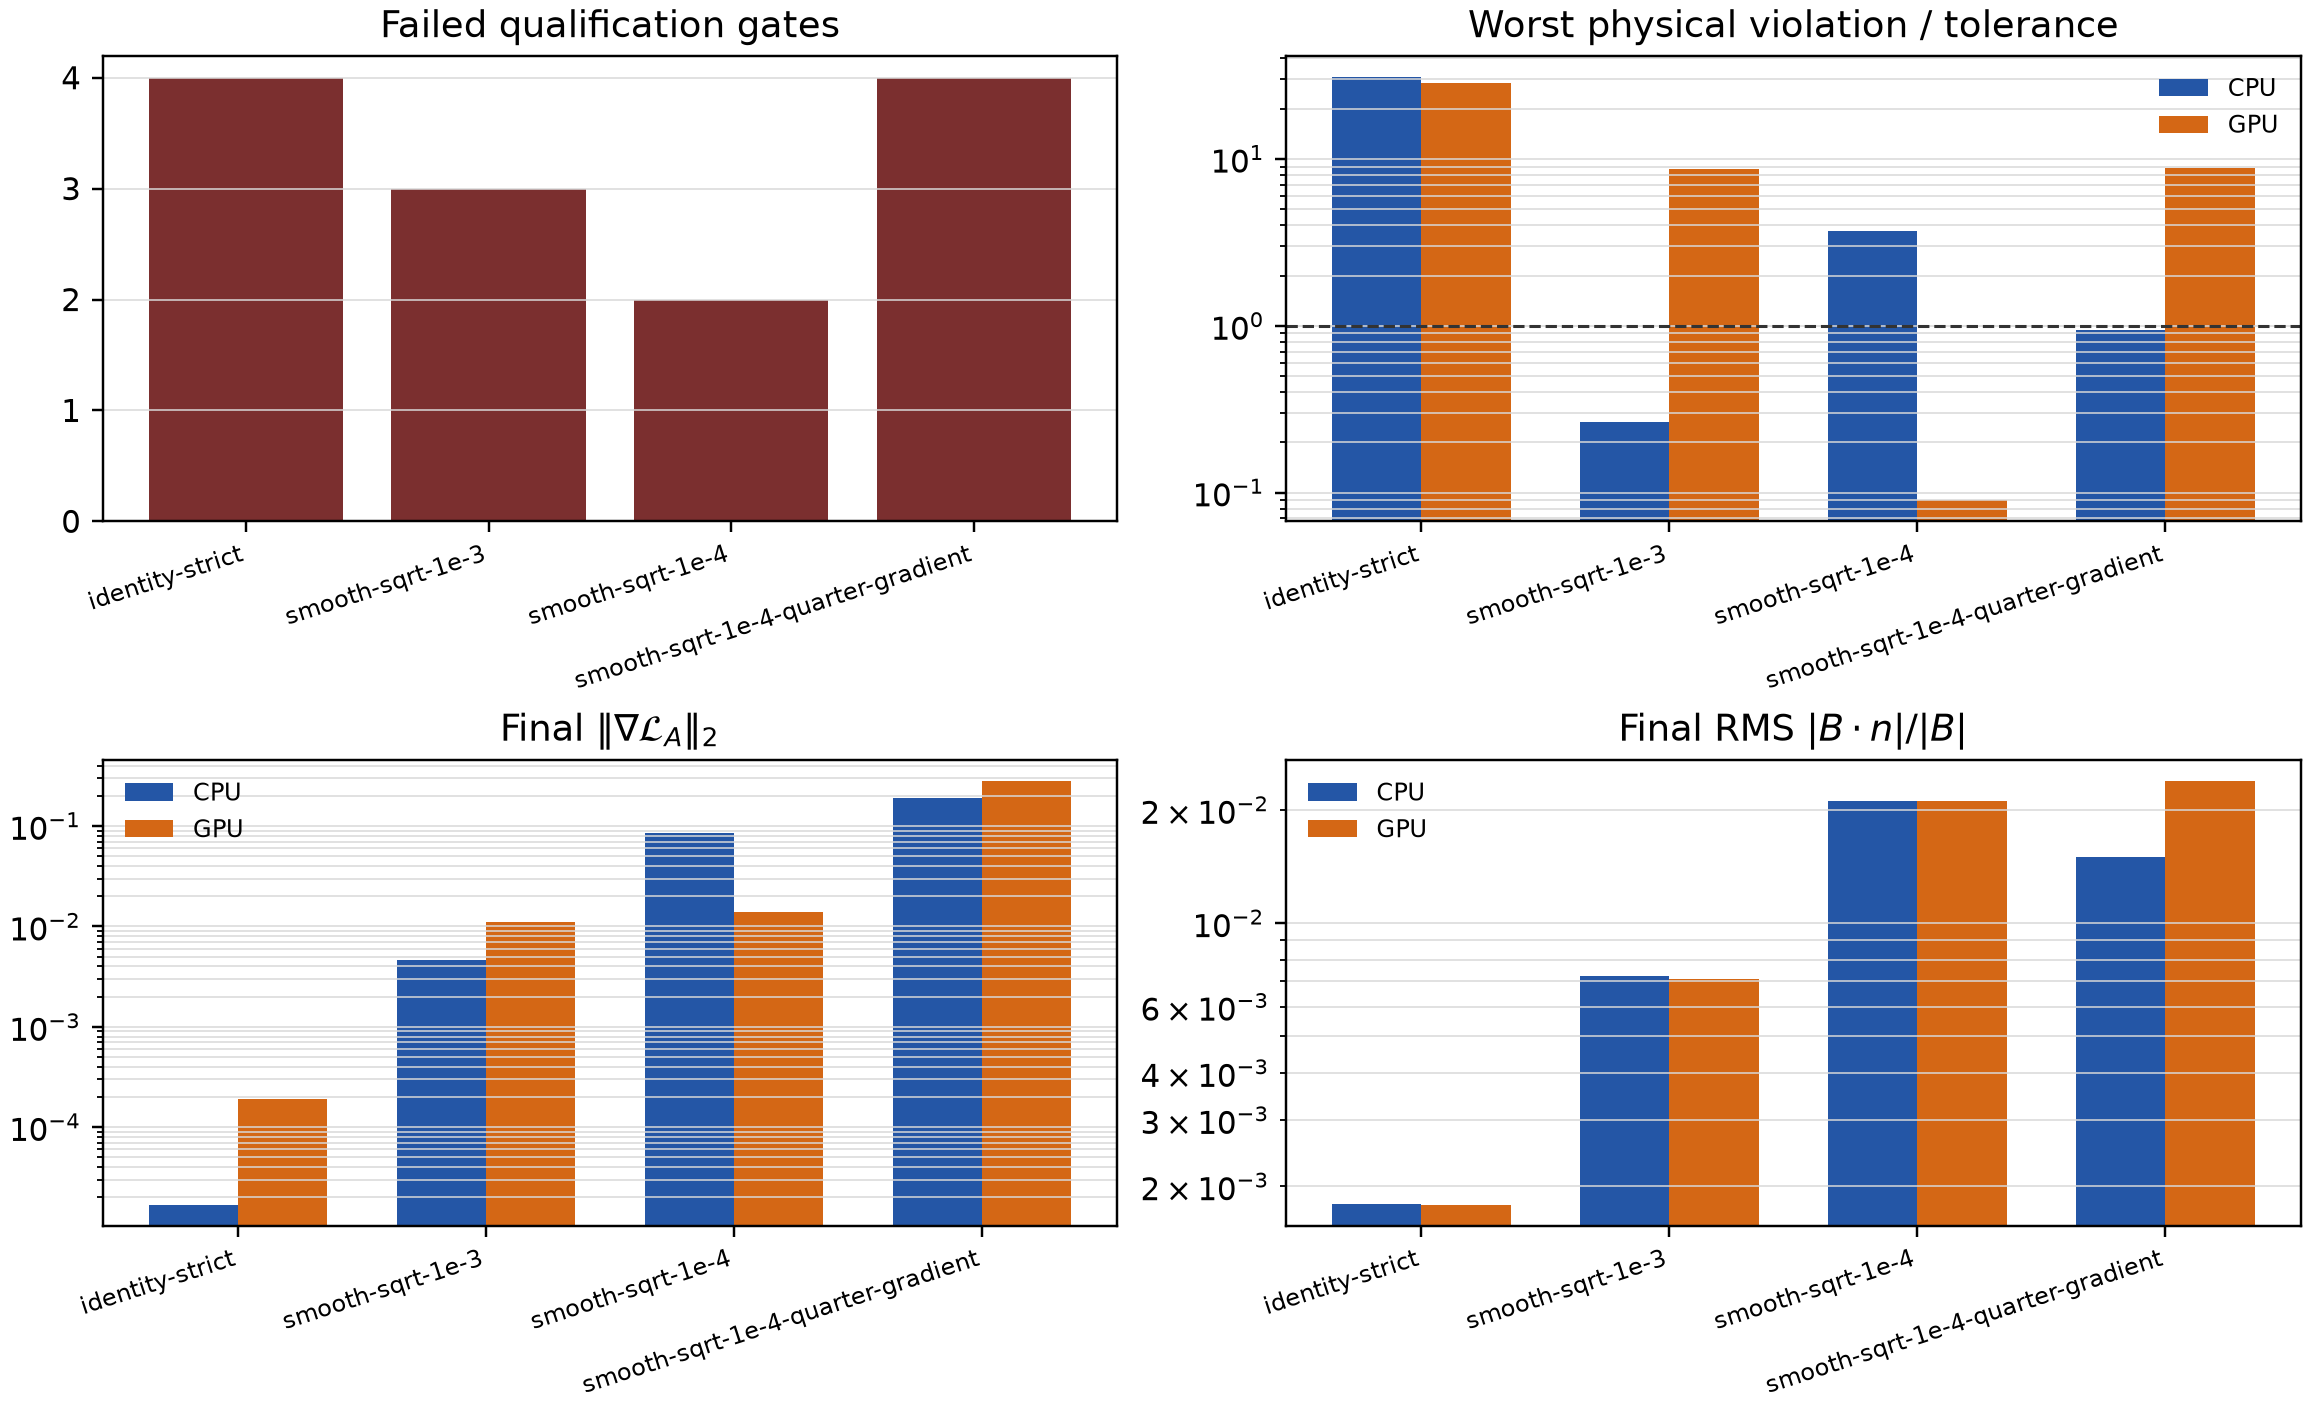
\includegraphics[width=\textwidth]{figures/al_safeguard_screen.png}
\caption{Hard qualification outcome on the engineering problem.  A dashed
ratio of one marks direct physical feasibility.  No candidate passes all
scientific gates; lower failed-gate count is diagnostic only.}
\label{fig:al-safeguard-screen}
\end{figure}

\begin{table}[htbp]
\centering
\caption{Safeguarded screening summary.  The gradient ratios divide the final
inner infinity-norm gradient by its requested tolerance.  A value above one
causes the safeguard to reject the stage.}
\label{tab:al-safeguard-screen}
\resizebox{\textwidth}{!}{%
\begin{tabular}{lrrrrrr}
\toprule
Candidate & failed gates & worst physical ratio & CPU grad/request &
GPU grad/request & CPU/GPU field RMS & warm speedup \\
\midrule
identity strict & 4 & 31.10 & 1.44 & 28.41 & 0.001794/0.001787 & 4.69 \\
$q_{\varepsilon}$, $\varepsilon=10^{-3}$ & 3 & 8.71 & 24.56 & 129.73 &
0.007218/0.007124 & 4.99 \\
$q_{\varepsilon}$, $\varepsilon=10^{-4}$ & 2 & 3.71 & 53.36 & 7.90 &
0.021090/0.021150 & 4.85 \\
$q_{\varepsilon}$, $\varepsilon=10^{-4}$, $\rho=0.25$ & 4 & 8.84 &
104.70 & 145.69 & 0.014973/0.023835 & 4.68 \\
\bottomrule
\end{tabular}}
\end{table}

All eight CPU/GPU solves eventually exhausted the 200-iteration inner budget.
Every final stage was marked nonstationary, no multiplier or penalty update
was applied, and production was correctly skipped.  This is the main success
of the implementation: the earlier failure mode would have continued
escalating penalties and reported a mechanical winner from these same states.
The safeguard instead turns false L-BFGS-B convergence into an explicit,
auditable termination.

The identity mapping gives the best field RMS and comes closest to CPU inner
stationarity, but is grossly infeasible: the worst direct violation is
31.10 times its allowance.  The $\varepsilon=10^{-4}$ residual-like mapping is
the best diagnostic candidate because it fails only feasibility and
stationarity.  Its GPU endpoint satisfies all stated direct physical
allowances, while the CPU coil--coil distance is 0.099629~m, a 0.371~mm
shortfall and 3.707 times the allowed distance deficit.  Its last CPU and GPU
gradient infinity norms are respectively $3.33\times10^{-2}$ and
$4.94\times10^{-3}$, against a requested $6.25\times10^{-4}$.

\begin{figure}[htbp]
\centering
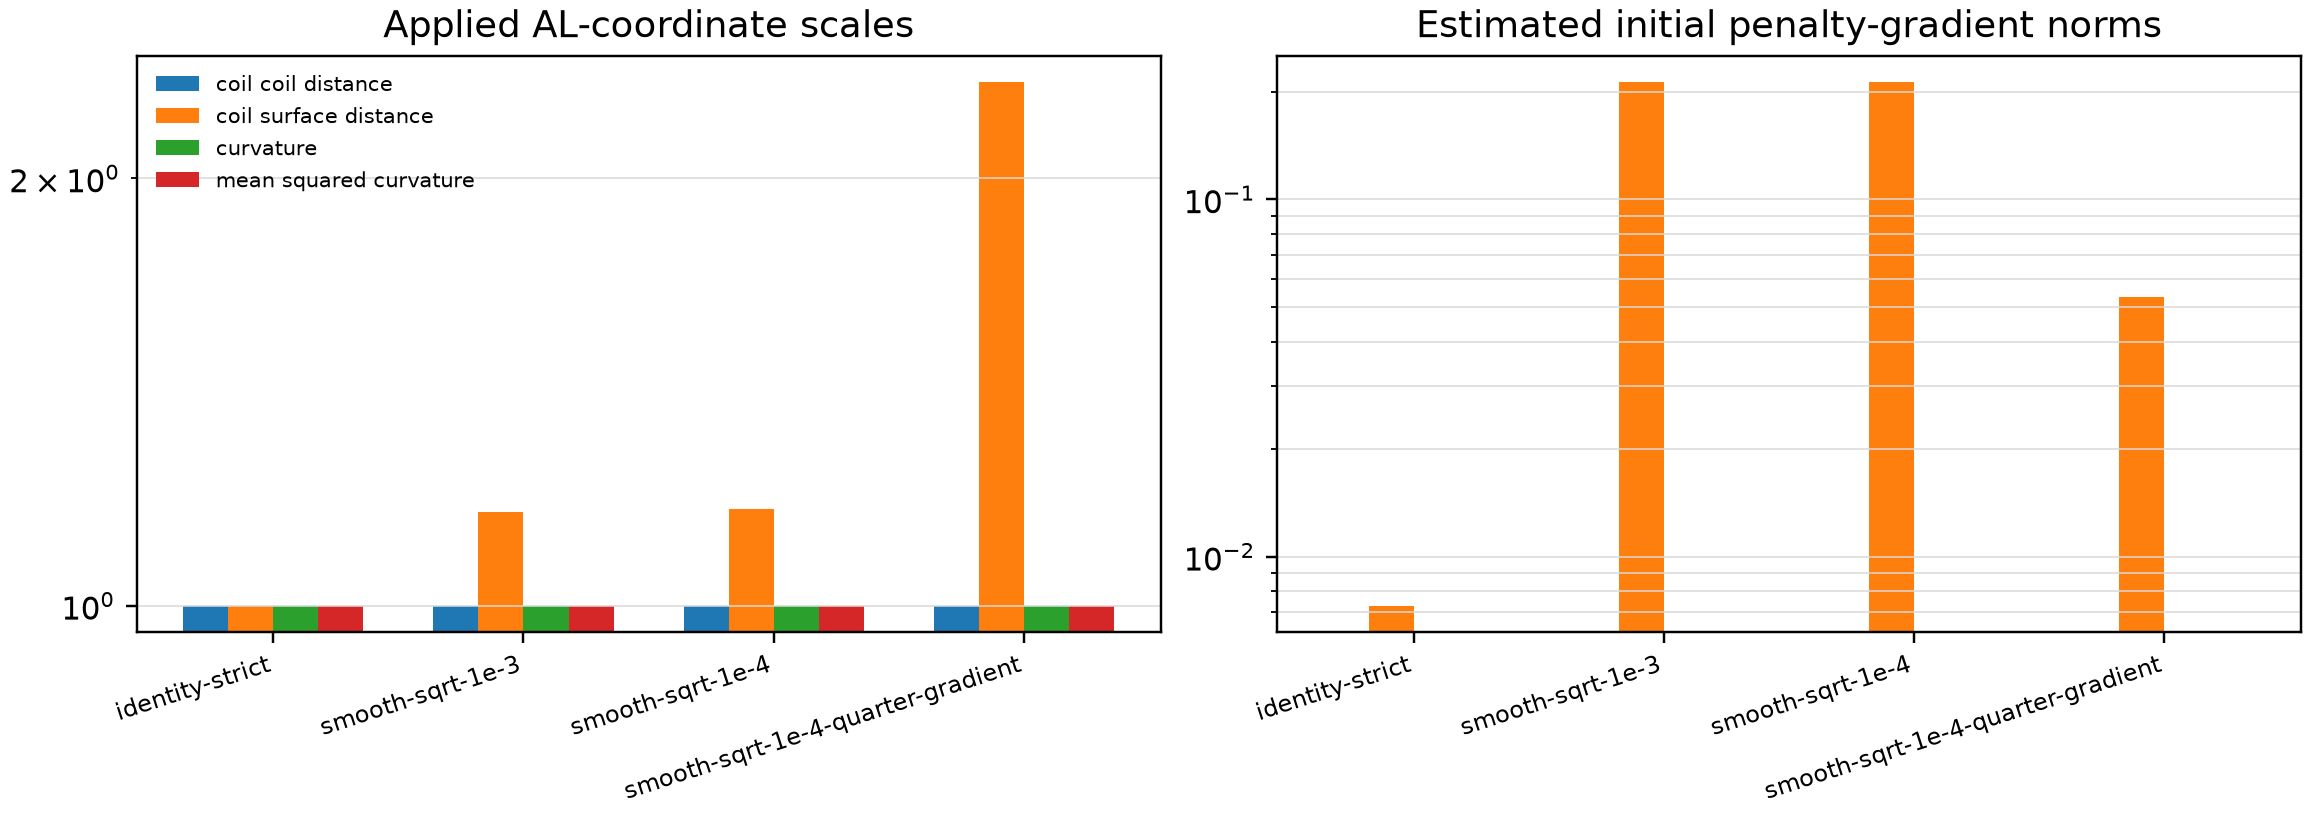
\includegraphics[width=\textwidth]{figures/al_safeguard_calibration.png}
\caption{One-shot gradient calibration.  Only coil--surface distance is active
at the canonical initial state, so the other three Jacobian rows contribute
zero and retain unit scale.  Constraints that activate later are therefore not
conditioned by this initialization-only rule.}
\label{fig:al-safeguard-calibration}
\end{figure}

The calibration plot explains an important limitation.  The initial base
gradient norm is 0.2137.  Under the identity map, the only nonzero estimated
constraint contribution is just 0.00729.  The square-root maps raise it to
0.2924 before attenuation; the selected scales 1.165--1.170 reduce it to the
base-gradient norm, while $\rho=0.25$ selects 2.339 and reduces it to 0.05343.
Coil--coil distance, curvature, and mean-squared curvature are inactive at
$x_0$, however, so one-shot Jacobian balancing cannot anticipate their later
activation.  The most aggressive attenuation also produces the largest
CPU/GPU gradient-to-request ratios and degrades endpoint agreement.

\begin{figure}[htbp]
\centering
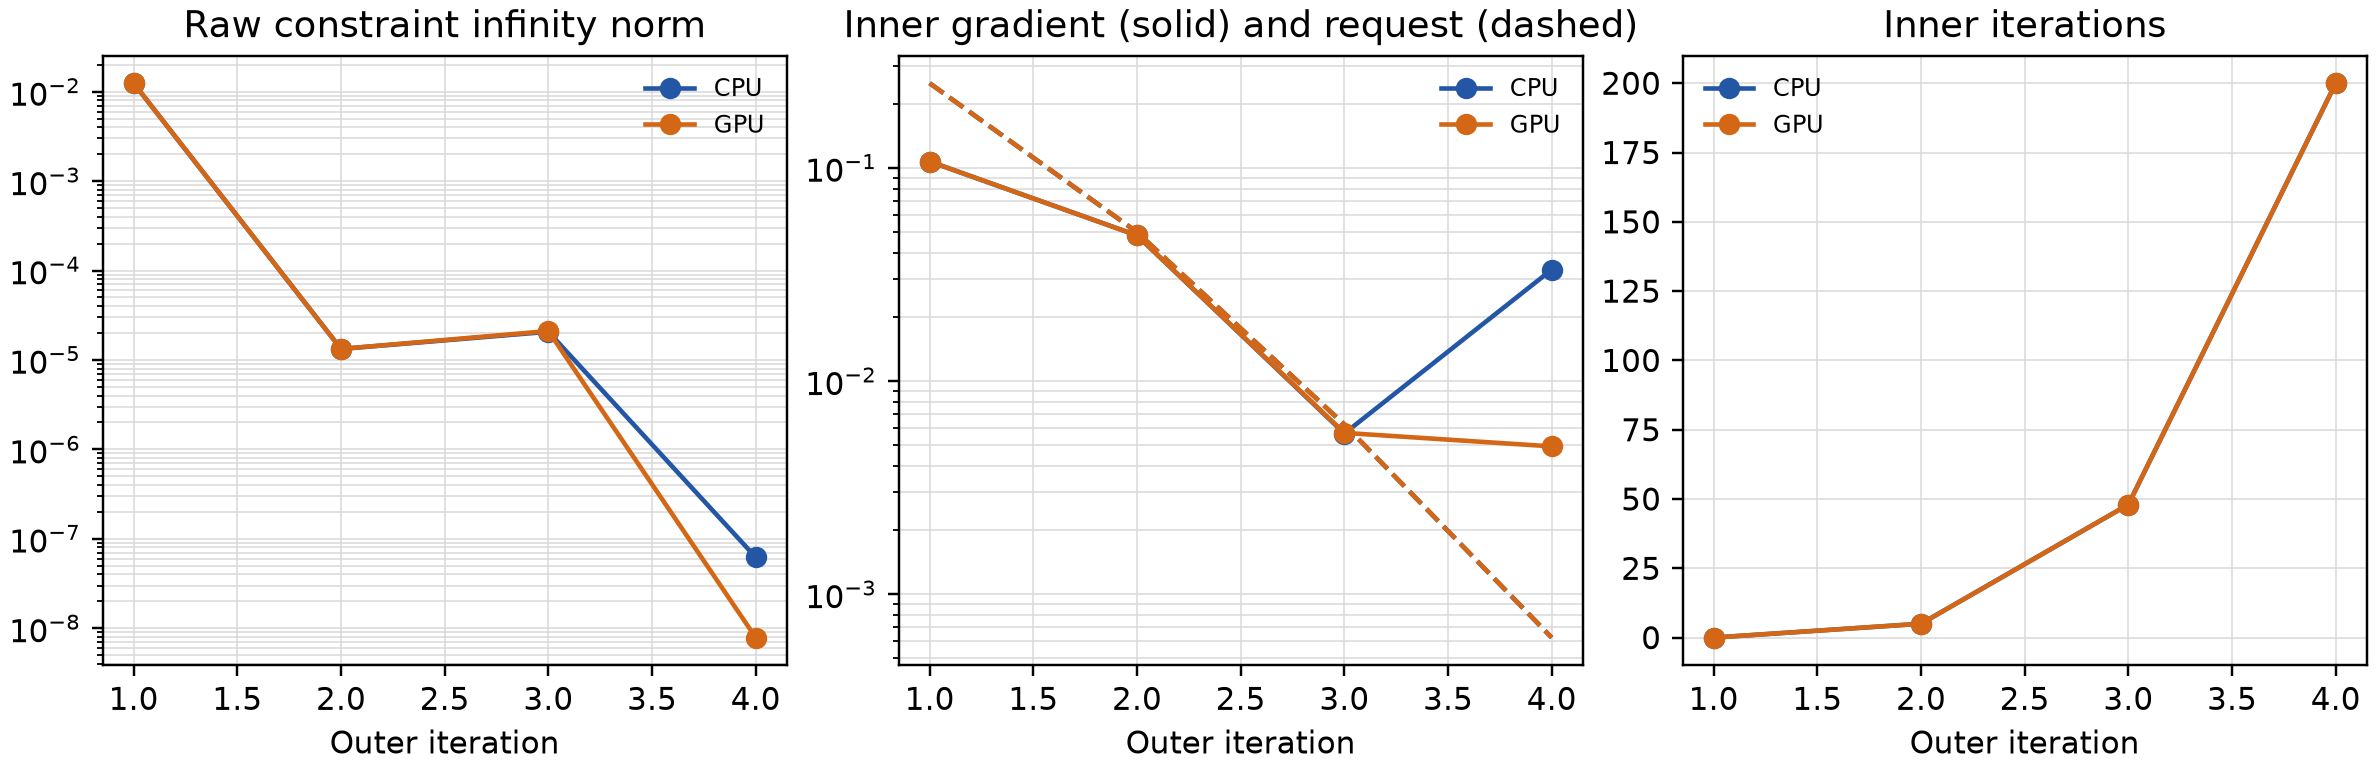
\includegraphics[width=\textwidth]{figures/al_safeguard_convergence.png}
\caption{Outer history for the best diagnostic screen,
$q_{\varepsilon}$ with $\varepsilon=10^{-4}$.  At outer step four both
backends reach the inner iteration cap while their gradient norms remain above
the dashed requested tolerance; the safe stop is therefore mandatory.}
\label{fig:al-safeguard-convergence}
\end{figure}

\begin{figure}[htbp]
\centering
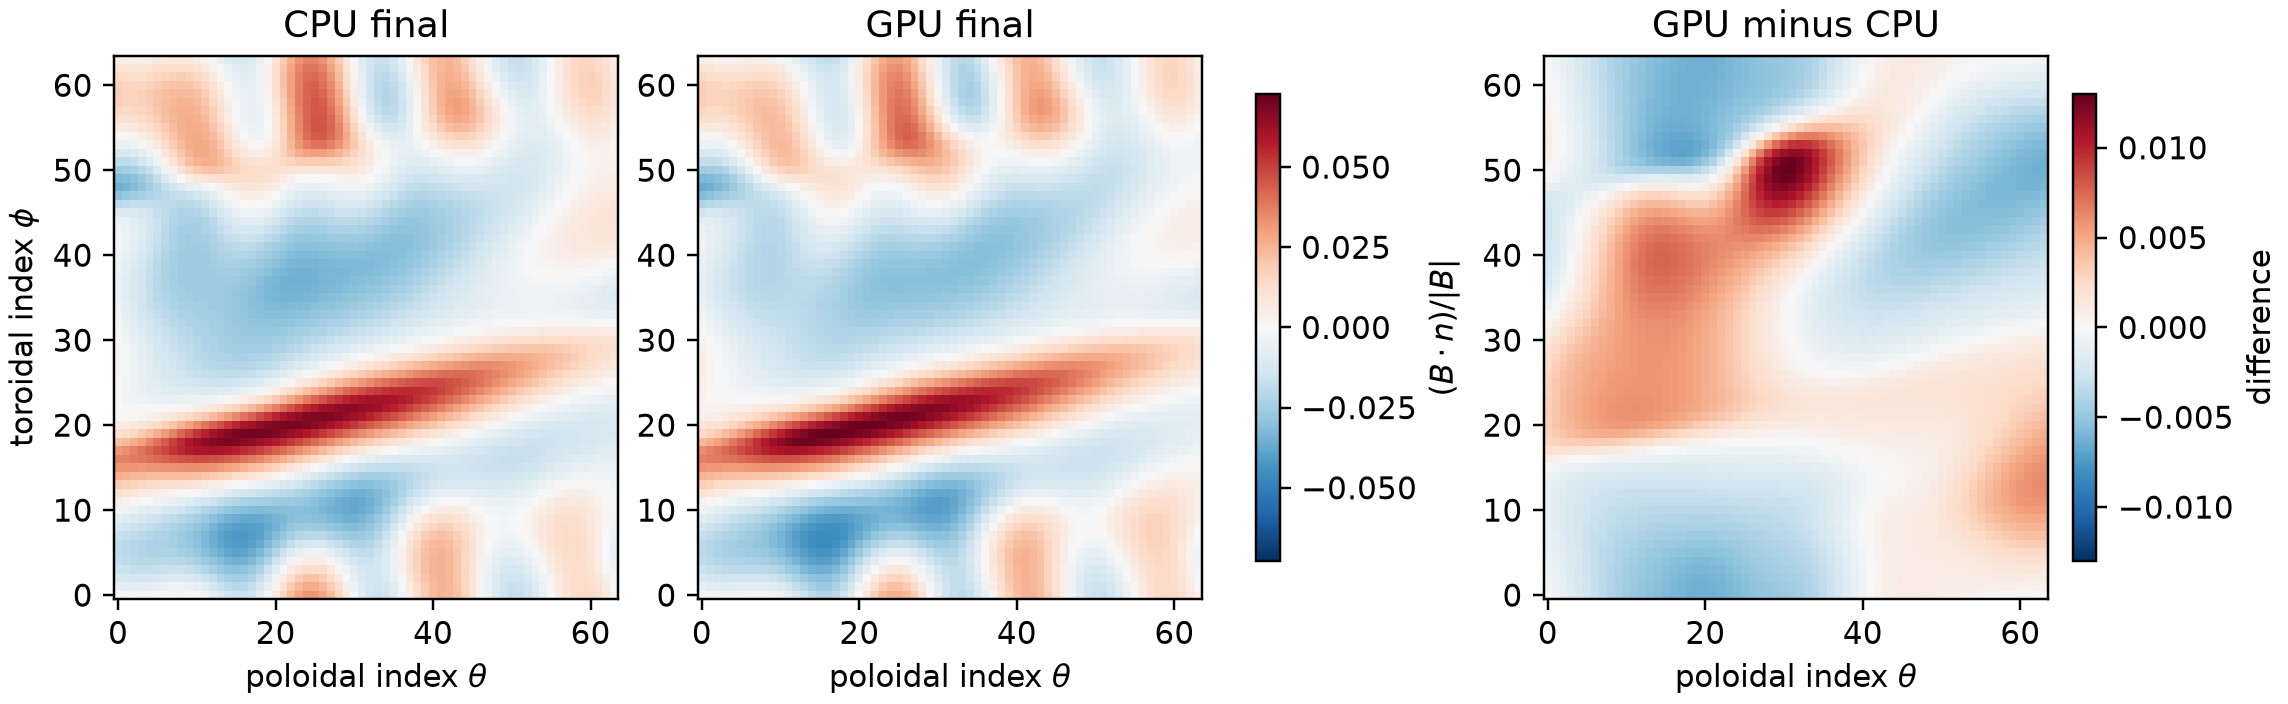
\includegraphics[width=\textwidth]{figures/al_safeguard_surface.png}
\caption{CPU and GPU signed $(B\cdot n)/|B|$ for the best diagnostic screen,
not an accepted production result.  Their signed correlation is 0.984 and
relative $L^2$ difference is 0.180; GPU has the smaller pointwise absolute
value on 46.2\% of surface points.}
\label{fig:al-safeguard-surface}
\end{figure}

The T4 still provides consistent throughput evidence.  Warm whole-run
speedups span 4.68--4.99, amortized speedups including compilation span
3.54--4.13, and time-per-physics-evaluation ratios span 4.25--4.62.  These are
kernel-throughput results, not equivalent-solution optimizer speedups, because
the CPU and GPU trajectories use different evaluation counts and no endpoint
qualified.

\textbf{Decision.}  Accept the strict safeguard, hard promotion rule,
schema-7 provenance, VTK exports, analyzer, and roughly $4.3$--$4.6\times$
per-evaluation acceleration.  Reject all four candidate designs and any
production or solution-quality claim.  A larger outer penalty or another
initial scalar-scale sweep is not justified.  The next implementation should
expose physically normalized, unsquared local hinge residuals before they are
aggregated.  Applying the AL quadratic to those residuals recovers the intended
second-order penalty instead of squaring an integrated squared penalty, and
lets newly active distance or curvature samples enter with explicit physical
units.  The experiment should retain the present safeguard and qualification
policy and first prove CPU/GPU value--Jacobian parity for the residual vector
before another optimization screen.

\section{Local residual qualification boundary}

The next implementation now exposes a fixed, device-resident residual vector
without changing the existing aggregate-penalty API.  Let $\epsilon_d$ be the
allowed distance violation, $\epsilon_\kappa$ the allowed curvature violation,
and $\epsilon_m$ the allowed mean-squared-curvature violation.  With nominal
limits $d_{cc}$, $d_{cs}$, $\kappa_{\max}$, and $m_{\max}$, the new residuals are
\begin{align}
r^{cc}_{ijq} &=\frac{\left[d_{cc}-\epsilon_d-
 \min_{q'}\|\gamma_{iq}-\gamma_{jq'}\|\right]_+}{\epsilon_d},\\
r^{cs}_{iq} &=\frac{\left[d_{cs}-\epsilon_d-
 \min_s\|\gamma_{iq}-S_s\|\right]_+}{\epsilon_d},\\
r^\kappa_{iq} &=\frac{\left[\kappa_{iq}-(\kappa_{\max}
 +\epsilon_\kappa)\right]_+}{\epsilon_\kappa},\\
r^m_i &=\frac{\left[m_i-(m_{\max}+\epsilon_m)\right]_+}{\epsilon_m}.
\end{align}
Thus $r=0$ is equivalent to the existing direct physical-feasibility allowance,
and a positive value reports violation in units of that allowance.  Applying an
AL quadratic to these unsquared hinges gives a second-order local penalty.  In
contrast, applying it to the earlier integrated squared penalty produces a
fourth-order response near feasibility and suppresses useful first-order
information.

\begin{figure}[htbp]
\centering
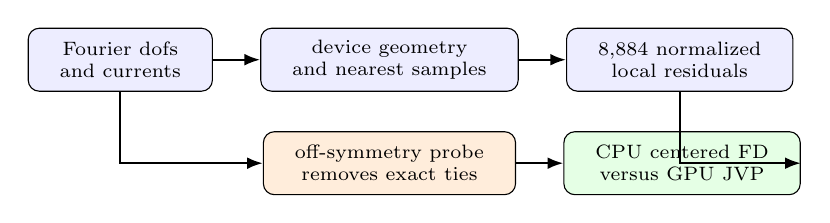
\begin{tikzpicture}[
  node distance=5mm and 6mm,
  box/.style={draw,rounded corners,align=center,minimum height=8mm,
              inner xsep=4mm,fill=blue!7,font=\scriptsize},
  probe/.style={draw,rounded corners,align=center,minimum height=8mm,
                inner xsep=4mm,fill=orange!14,font=\scriptsize},
  gate/.style={draw,rounded corners,align=center,minimum height=8mm,
               inner xsep=4mm,fill=green!10,font=\scriptsize},
  flow/.style={-{Latex[length=2mm]},thick}
]
\node[box] (geometry) {Fourier dofs\\and currents};
\node[box,right=of geometry] (samples) {device geometry\\and nearest samples};
\node[box,right=of samples] (residuals) {8,884 normalized\\local residuals};
\node[probe,below=of samples] (probe) {off-symmetry probe\\removes exact ties};
\node[gate,right=of probe] (parity) {CPU centered FD\\versus GPU JVP};
\draw[flow] (geometry) -- (samples);
\draw[flow] (samples) -- (residuals);
\draw[flow] (probe) -- (parity);
\draw[flow] (geometry.south) |- (probe.west);
\draw[flow] (residuals.south) |- (parity.east);
\end{tikzpicture}
\caption{Residual qualification precedes optimizer integration.  Production
values are checked at the unmodified initial point; directional derivatives are
checked at a documented $10^{-4}$ off-symmetry geometry probe because an exact
nearest-neighbor tie has no unique classical Jacobian.}
\label{fig:local-residual-boundary}
\end{figure}

The engineering layout contains 6,480 coil--coil entries, 1,920 coil--surface
entries, 480 curvature entries, and four mean-squared-curvature entries, for
8,884 residuals total.  The stress layout remains modest at 27,546 entries.
Coil--surface nearest distances are reduced in target tiles, so neither layout
materializes the full coil-point--surface interaction matrix.  Named, contiguous
family slices are part of the public experimental contract and allow familywise
scaling, diagnostics, and matrix-free products without a dense Jacobian.

Unit coverage now checks each primitive, tiled versus full nearest-distance
values, the composed objective boundary, stable family offsets, and the
independent NumPy oracle.  Nineteen focused tests and all 104 GPU-module tests
pass locally.  An engineering CPU-only smoke run additionally gives
$1.1\times10^{-16}$ relative
forced-residual value error and $1.6\times10^{-9}$ relative
directional-Jacobian error between the two
implementations; this validates the harness but is not NVIDIA performance
evidence.  The Colab workflow records float64 hardware provenance, production
and forced-activation value parity, three directional JVP checks, compilation,
warm timing, and all acceptance gates.  Its analyzer validates a returned ZIP
and produces one four-panel activation, magnitude, Jacobian, and performance
figure.

Exact symmetry points remain valid for value tests; a deterministic
off-symmetry probe is required only when claiming a classical Jacobian
comparison.

\subsection{NVIDIA qualification result}

The returned archive was produced from revision \code{9849fb4c}.  Its SHA-256
is:
\begin{center}
\small\ttfamily
d0d372935ca9b1a695a6ecaf8c18527c\\
7110b830e5e393b766fe6e9d7e0389b6
\end{center}
It records Linux, Python 3.13.15, JAX 0.11.1, one
\code{cuda:0} device, float64, and one OpenMP thread.  The exact accelerator
model was not recorded, so this result is correctly described as an NVIDIA
CUDA result rather than attributed to a particular GPU.  Device-kind metadata
has now been added to the shared environment recorder for subsequent archives.

\begin{table}[htbp]
\centering
\caption{Measured engineering-scale local-residual qualification.  Every gate
passes; smaller parity errors are better.}
\label{tab:local-residual-qualification}
\begin{tabular}{lrr}
\toprule
Quantity & Observed & Gate \\
\midrule
Base-objective relative error & $1.26\times10^{-15}$ & $\leq5\times10^{-10}$ \\
Production-residual relative $L^2$ error & $4.10\times10^{-16}$ & $\leq5\times10^{-10}$ \\
Forced-residual relative $L^2$ error & $1.76\times10^{-16}$ & $\leq5\times10^{-10}$ \\
Worst directional-Jacobian relative $L^2$ error & $1.60\times10^{-9}$ & $\leq5\times10^{-4}$ \\
CPU warm median & 348.553 ms & --- \\
GPU warm median & 30.775 ms & --- \\
Warm term-evaluation speedup & $11.326\times$ & report \\
GPU compilation & 1.713 s & report \\
\bottomrule
\end{tabular}
\end{table}

\begin{figure}[htbp]
\centering
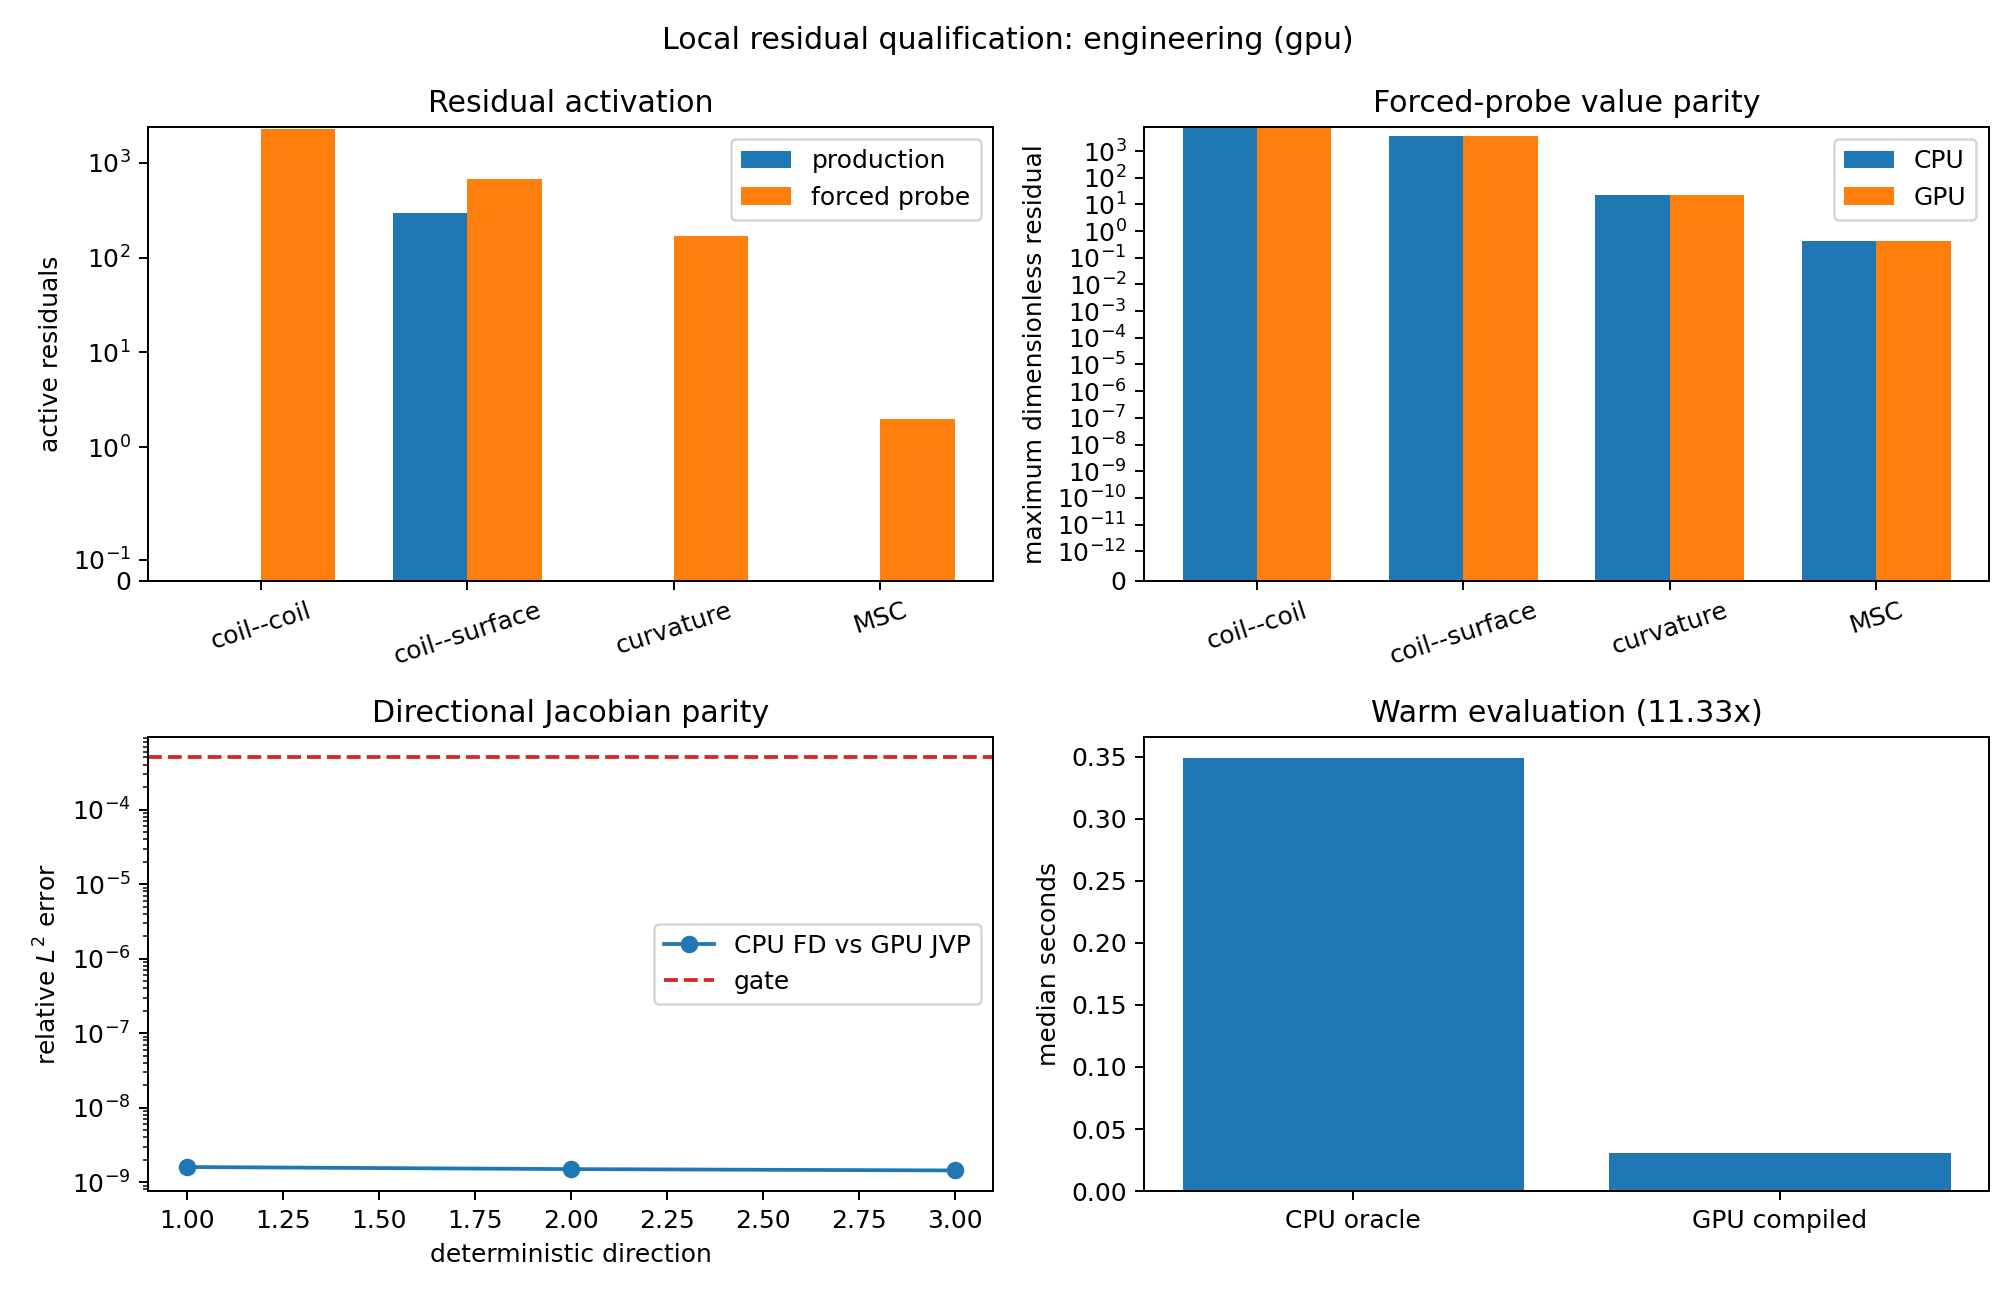
\includegraphics[width=\textwidth]{figures/local_residual_parity.png}
\caption{Measured local-residual qualification.  The production initial point
activates 294 of 1,920 coil--surface residuals and no other family.  The forced
probe activates every family; CPU and GPU maxima overlay visually, all three
Jacobian errors are near $1.5\times10^{-9}$, and warm term evaluation is
$11.33\times$ faster on the recorded CUDA device.}
\label{fig:local-residual-qualification}
\end{figure}

The production-threshold result is also diagnostically useful.  Coil--coil,
curvature, and mean-squared-curvature residuals are all zero, while 294
coil--surface samples are active.  Their maximum normalized residual is
1,869.19, corresponding to a 0.186919 m deficit relative to the allowed
0.2999 m sampled separation.  The forced probe then activates 2,298
coil--coil, 672 coil--surface, 168 curvature, and two mean-squared-curvature
entries.  This proves parity for active derivatives in every family rather than
passing only because most production hinges are inactive.

\textbf{Decision.}  Accept all local-residual value, active-family,
directional-Jacobian, dimension, and backend gates.  Keep the original
aggregate constraints for backward compatibility, promote the normalized local
residual vector to the safeguarded optimizer boundary, and proceed to a matched
CPU/GPU optimization screen.  The $11.33\times$ number is accepted as
term-evaluation throughput, not yet as optimizer or equivalent-solution
speedup.  The next optimization archive must restore the full final metric
contract and export CPU/GPU surface VTS and coil VTU artifacts.

\subsection{Local-residual optimizer integration}

That optimizer boundary is now implemented.  Let $r(x)\in\mathbb{R}^m_+$ be
the qualified local residual vector and let $s\in\mathbb{R}^m_+$ contain fixed
scales.  The new matched CPU/GPU experiment minimizes
\begin{equation}
 \mathcal{L}_A(x,\lambda,\mu)
 = f(x)-\lambda^T\widehat r(x)
   +\frac{1}{2}\sum_{j=1}^{m}\mu_j\widehat r_j(x)^2,
 \qquad \widehat r_j=r_j/s_j.
\end{equation}
The reverse pass directly evaluates
$J_r(x)^T[-\lambda+\mu\odot\widehat r]/s$ through JAX.  No dense
$m\times n$ residual Jacobian is formed or stored.  This distinction matters:
the engineering case has $m=8{,}884$ residuals but only a few hundred optimizer
coordinates, and a future high-resolution case increases $m$ much faster than
$n$.

CPU and GPU now execute the same residual and derivative program, explicitly
lowered to a JAX CPU device and an NVIDIA GPU device respectively.  This makes
the timing question precise: it measures backend execution rather than mixing
a SIMSOPT derivative graph on CPU with JAX automatic differentiation on GPU.
The independent NumPy/SIMSOPT values and finite-difference directional
derivatives in the preceding qualification remain the implementation oracle.

\begin{figure}[htbp]
\centering
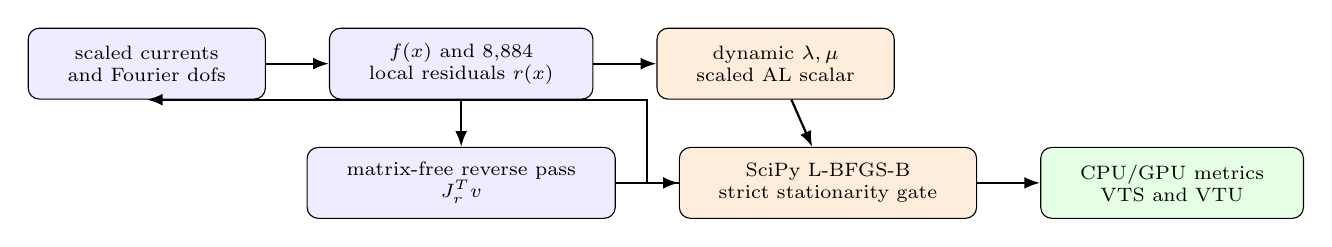
\begin{tikzpicture}[
  node distance=6mm and 8mm,
  box/.style={draw,rounded corners,align=center,minimum height=9mm,
              inner xsep=5mm,fill=blue!7,font=\scriptsize},
  state/.style={draw,rounded corners,align=center,minimum height=9mm,
                inner xsep=5mm,fill=orange!14,font=\scriptsize},
  output/.style={draw,rounded corners,align=center,minimum height=9mm,
                 inner xsep=5mm,fill=green!10,font=\scriptsize},
  flow/.style={-{Latex[length=2mm]},thick}
]
\node[box] (x) {scaled currents\\and Fourier dofs};
\node[box,right=of x] (terms) {$f(x)$ and $8{,}884$\\local residuals $r(x)$};
\node[state,right=of terms] (al) {dynamic $\lambda,\mu$\\scaled AL scalar};
\node[box,below=of terms] (vjp) {matrix-free reverse pass\\$J_r^T v$};
\node[state,right=of vjp] (lbfgs) {SciPy L-BFGS-B\\strict stationarity gate};
\node[output,right=of lbfgs] (artifacts) {CPU/GPU metrics\\VTS and VTU};
\draw[flow] (x) -- (terms);
\draw[flow] (terms) -- (al);
\draw[flow] (al) -- (lbfgs);
\draw[flow] (terms) -- (vjp);
\draw[flow] (vjp) -- (lbfgs);
\draw[flow] (lbfgs) -- (artifacts);
\draw[flow] (lbfgs.west) -- ++(-4mm,0) |- (x.south);
\end{tikzpicture}
\caption{Implemented local-residual AL data path.  Only the optimizer vector,
scalar value, and gradient cross the SciPy boundary.  Constraint state remains
dynamic executable input, while final scientific metrics and visualization
artifacts are evaluated through the common SIMSOPT CPU oracle.}
\label{fig:local-residual-al-data-path}
\end{figure}

The selected family scale is
\begin{equation}
 s_j=s_k=\max\!\left(1,\sqrt{m_k},
               \lVert r^{(k)}(x_0)\rVert_2\right),
 \qquad j\in\text{family }k.
\end{equation}
It is attenuation-only.  For an initially active family it bounds
$\lVert\widehat r^{(k)}(x_0)\rVert_2$ by one; for an inactive family the
$\sqrt{m_k}$ floor prevents a later vector of order-one residuals from receiving
an artificial factor of $m_k$ merely because the family contains many samples.
Scaling never changes the raw stopping test or the direct physical-feasibility
gate.

One additional scheduler decision is necessary.  The earlier componentwise
penalty update is retained as the general default, but this experiment uses a
global update: if any raw local residual exceeds tolerance, all entries of
$\mu$ grow together.  With componentwise updates, thousands of inactive entries
would remain at $\mu_0$ and make the mean-penalty accuracy schedule advance only
weakly.  Global growth preserves the scalar-penalty behavior of the supplied
reference algorithm while retaining per-residual multipliers.

The outer history now supports a compact mode.  Every stage records the size,
nonzero count, minimum, maximum, $L^2$ norm, and infinity norm of residuals,
scaled residuals, multipliers, and penalties instead of serializing six vectors
of length 8,884.  Named final family summaries remain in the result.  Strict
inner stationarity is mandatory; a nonstationary L-BFGS-B endpoint cannot
update $\lambda$ or $\mu$.

The complete final-state contract has also been restored.  Both endpoints
record the legacy full objective, mean/RMS/maximum
$|B\cdot n|/|B|$, all coil measurements, margins, and violations through one
SIMSOPT CPU oracle.  Each endpoint exports a VTS surface containing signed and
absolute normalized normal-field arrays and a VTU file containing all physical
coils.  The analyzer validates these artifacts and produces convergence,
performance, and surface-comparison figures.

A CPU-only minimal smoke run compiled both explicitly selected CPU executables,
gave exactly equal initial values, residuals, AL values, and gradients, retained
the 5,554-entry compact history contract, evaluated both complete final metric
snapshots, and stopped safely after the deliberately tiny two-iteration inner
budget.  This is structural validation only, not performance or solution
evidence.

\textbf{Decision.}  Run the engineering-scale notebook before attempting the
27,546-residual stress problem.  Promotion requires the NVIDIA backend and
initial parity gates, raw local-residual and direct physical feasibility,
strict stationary convergence on both backends, CPU-relative field and
constraint quality, the physics-evaluation budget, and at least $3\times$ warm
optimization speedup.  The archive is retained even if a scientific gate fails;
the next design decision will be based on its measured family endpoints and
not on timing alone.

\subsubsection{A100 engineering qualification result}

The returned archive was produced from revision \code{423a4f6e} on one NVIDIA
A100-SXM4-40GB with driver 580.82.07, JAX 0.11.1, Python 3.13.15, float64, and
one OpenMP thread.  Its SHA-256 is:
\begin{center}
\small\ttfamily
444f179a1319f59d8c9a124abcefafb9\allowbreak
6bc4529172da23892e16ff83018c2e36
\end{center}
All four VTK files are nonempty and the analyzer independently validates the
8,884-residual layout, compact histories, final metric contract, and surface
point arrays.

Initial CPU/GPU agreement is at roundoff: base-objective absolute error is
$6.94\times10^{-18}$, residual relative $L^2$ error is
$1.20\times10^{-16}$, and AL-gradient relative $L^2$ error is
$1.19\times10^{-16}$.  The archive therefore confirms that the explicitly
pinned CPU and GPU executables begin from the same mathematical problem.

\begin{table}[htbp]
\centering
\caption{Measured local-residual AL endpoints on the engineering problem.
Neither endpoint is accepted because stationarity and feasibility gates fail.}
\label{tab:local-residual-al-result}
\begin{tabular}{lrr}
\toprule
Quantity & CPU & GPU \\
\midrule
Solve time (s) & 499.412 & 6.225 \\
Physics evaluations & 705 & 914 \\
Outer / total inner iterations & 2 / 245 & 2 / 173 \\
Final base objective & 0.0165123 & 0.0162893 \\
Final gradient infinity norm & 0.02933 & 205.916 \\
Raw residual infinity norm & 0.245661 & $5.023\times10^{-5}$ \\
$|B\cdot n|/|B|$ mean & 0.164378 & 0.163532 \\
$|B\cdot n|/|B|$ RMS & 0.191970 & 0.190910 \\
$|B\cdot n|/|B|$ maximum & 0.383547 & 0.380934 \\
Minimum coil--coil distance (m) & 0.114532 & 0.114235 \\
Minimum coil--surface distance (m) & 0.299875 & 0.299900 \\
Maximum curvature (m$^{-1}$) & 4.14766 & 4.17179 \\
Maximum mean-squared curvature (m$^{-2}$) & 5.0010000 & 5.0010001 \\
\bottomrule
\end{tabular}
\end{table}

\begin{figure}[htbp]
\centering
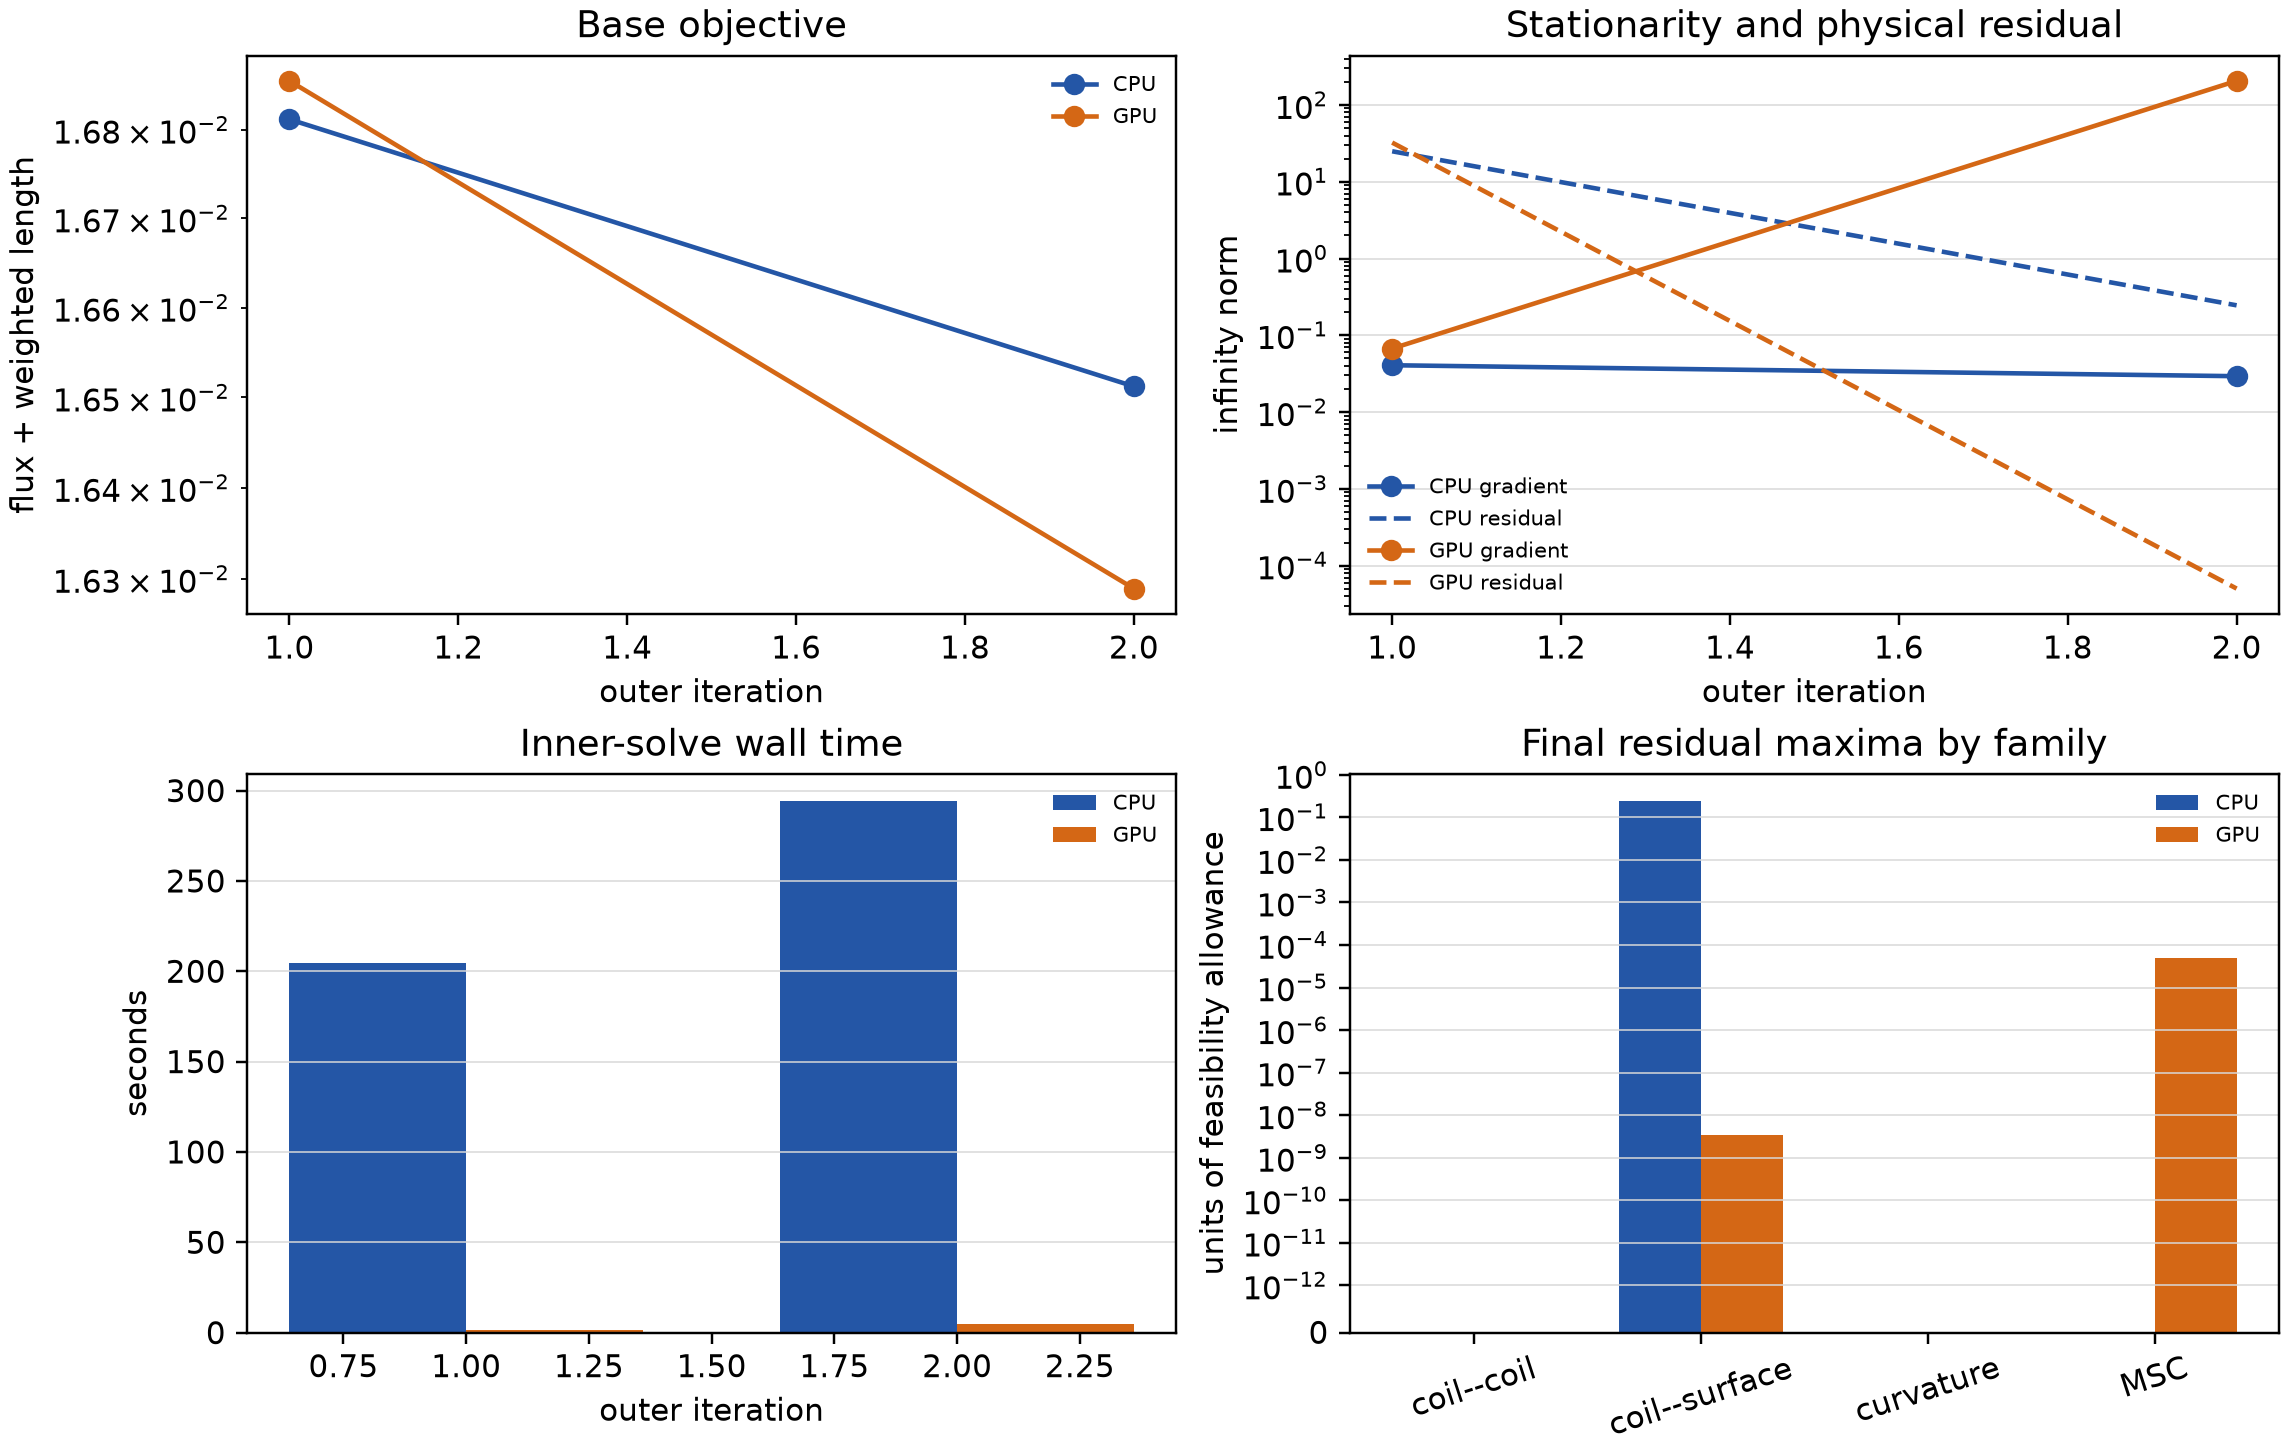
\includegraphics[width=\textwidth]{figures/local_residual_al_convergence.png}
\caption{Measured local-residual AL history.  Both first inner solves satisfy
their requested $10^{-1}$ infinity-norm stationarity tolerance and permit one
outer update.  At the second stage, CPU exhausts 200 iterations at gradient
infinity norm 0.0293; GPU reports function-reduction termination but has
gradient infinity norm 205.9.  The safeguard correctly rejects both returns.}
\label{fig:local-residual-al-convergence}
\end{figure}

The CPU endpoint has one active coil--surface residual of 0.245661.  In physical
terms its minimum separation is 0.29987543~m, so the deficit from the nominal
0.3~m limit is 0.124566~mm and exceeds the allowed 0.1~mm deficit by
0.024566~mm.  The GPU endpoint reduces its coil--surface residual to
$3.41\times10^{-9}$, but one mean-squared-curvature residual remains
$5.02\times10^{-5}$.  The direct oracle correspondingly reports an MSC excess
of 0.001000050, just $5.02\times10^{-8}$ beyond its allowance.  Its
coil--surface deficit is 0.10000000034~mm, only $3.4\times10^{-10}$~m beyond
the boundary.  These near-boundary values are diagnostically encouraging but
must not be rounded into passing results.

\begin{figure}[htbp]
\centering
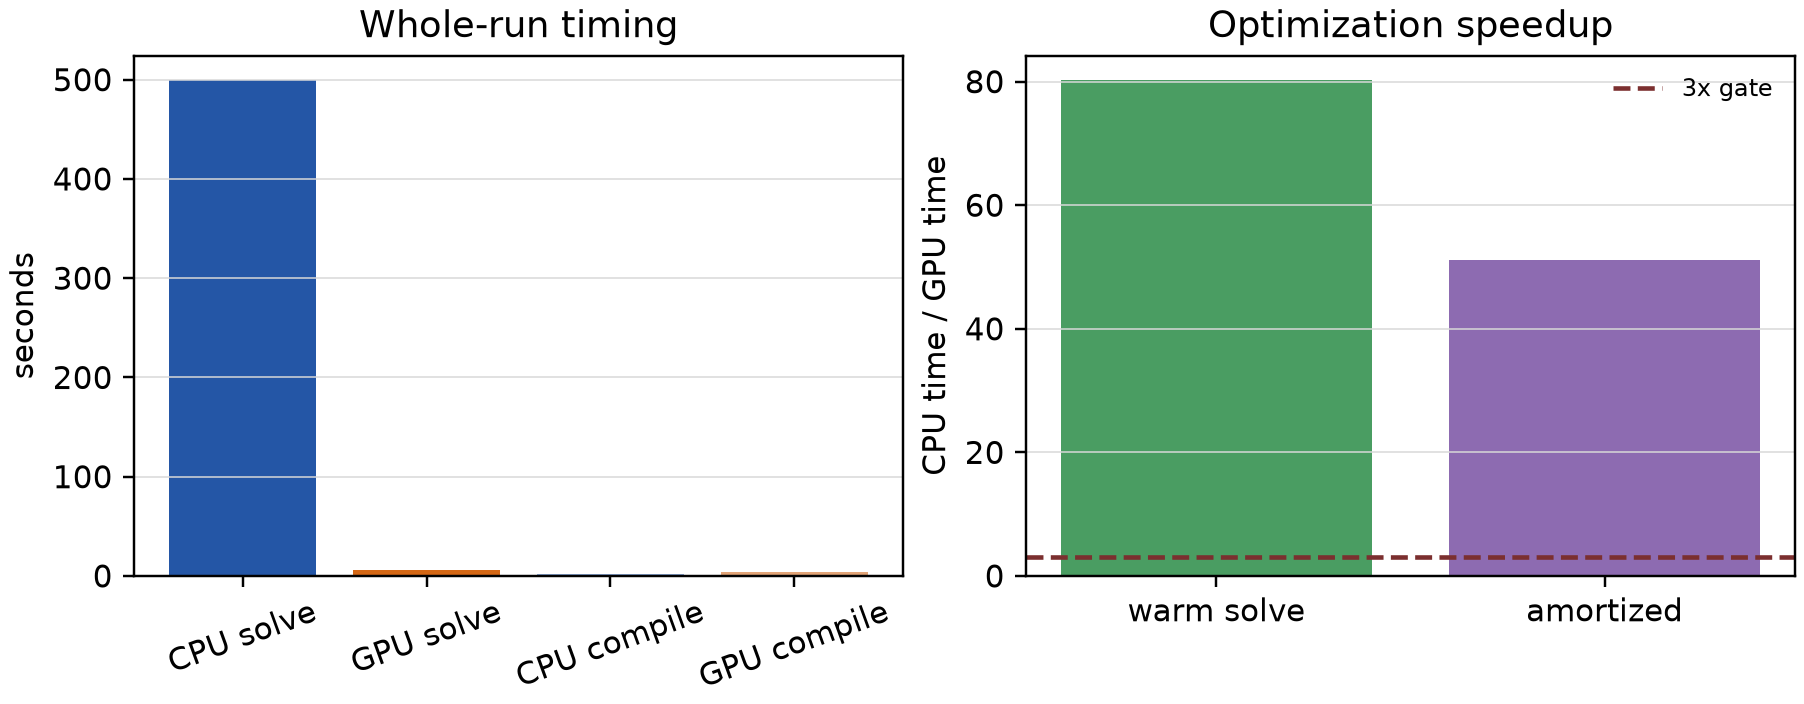
\includegraphics[width=0.92\textwidth]{figures/local_residual_al_performance.png}
\caption{A100 timing for the nonqualifying trajectories.  Warm whole-solve
speedup is $80.22\times$ and speedup including 3.541~s GPU compilation is
$51.14\times$.  Different evaluation counts and failed stationarity mean these
are throughput measurements, not equivalent-solution speedups.}
\label{fig:local-residual-al-performance}
\end{figure}

The field and relative-quality gates pass.  GPU normalized-normal-field mean,
RMS, and maximum are respectively 0.5--0.7\% below the CPU values.  The two
signed surface maps have correlation 0.999974, relative $L^2$ difference
0.00906, and maximum pointwise difference 0.00488.  The physics-evaluation
budget fails because GPU uses 914 evaluations versus the allowed
$\lceil1.1\times705\rceil=776$.

\begin{figure}[htbp]
\centering
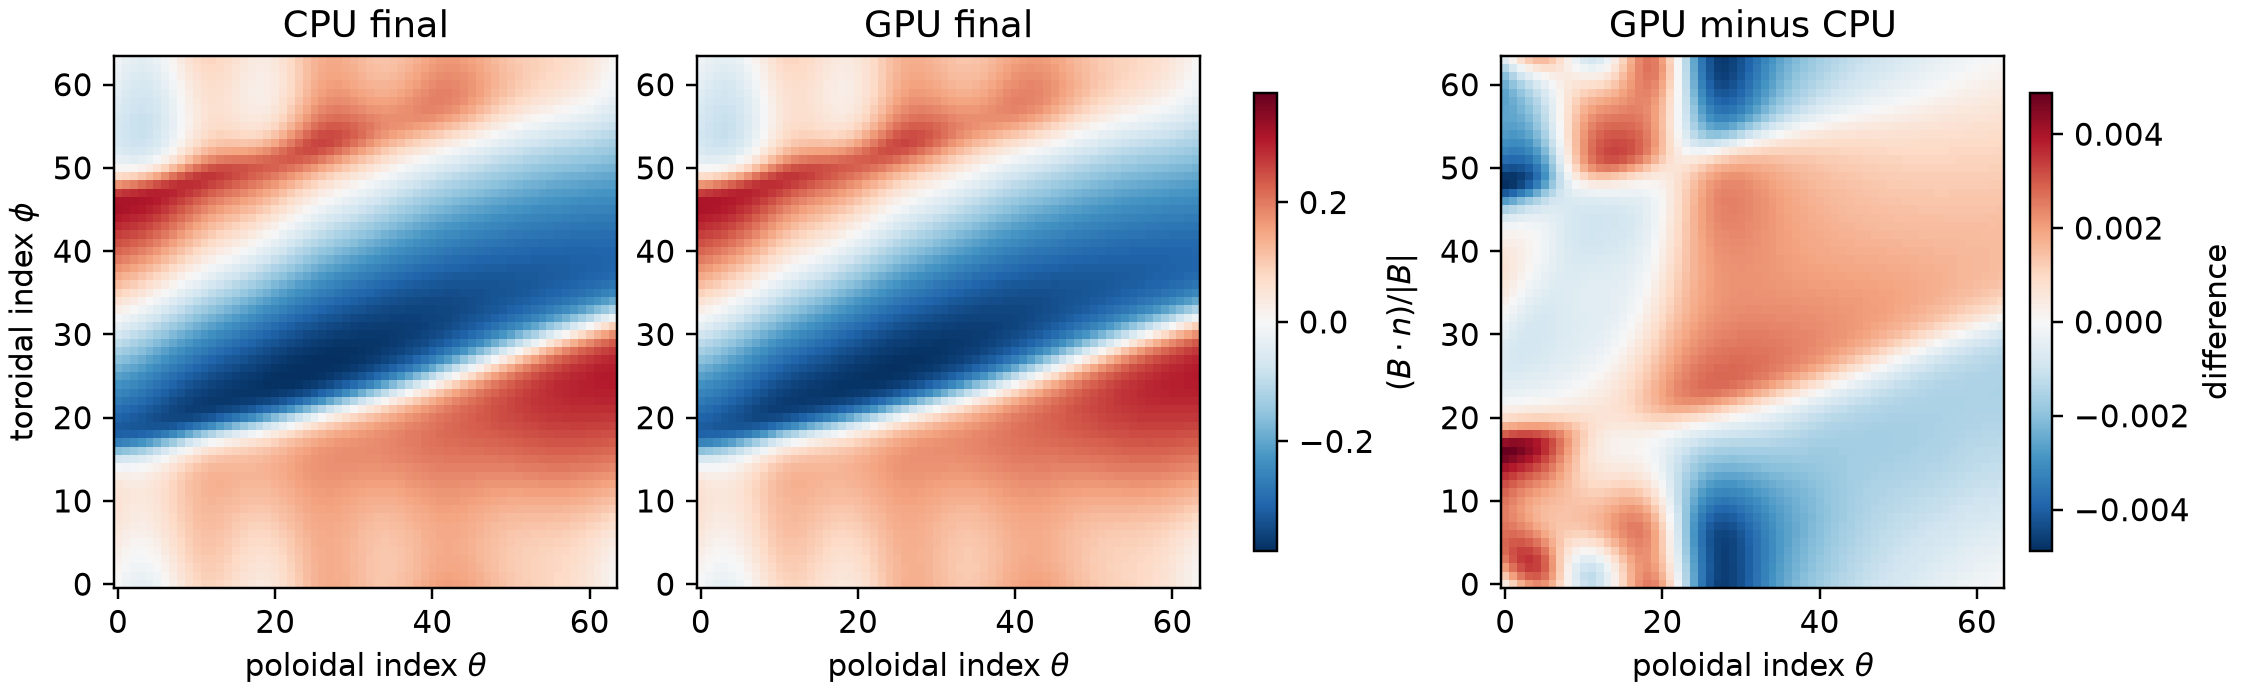
\includegraphics[width=\textwidth]{figures/local_residual_al_surface.png}
\caption{Final signed $(B\cdot n)/|B|$ maps from the two rejected endpoints.
The close maps show that the physical designs remain similar even though the
second-stage line searches terminate very differently.}
\label{fig:local-residual-al-surface}
\end{figure}

The failure exposes two conditioning mechanisms.  First, the initial
coil--surface family scale is 18,498 because that family begins with a very
large residual norm.  Near feasibility, this fixed scale attenuates the
remaining raw constraint by the same factor, so the AL progress coordinate can
look extremely small while the physical residual still fails.  Second, after
the first multiplier update the linear term in a ReLU hinge introduces a kink
at its zero boundary.  L-BFGS-B can then report relative function reduction
without stationarity, as observed on GPU.  Merely increasing penalties or
promoting to the stress problem would compound these effects.

\textbf{Decision.}  Accept backend parity, VTK/metric completeness, the compact
matrix-free implementation, field/relative-constraint quality, and the A100
throughput evidence.  Reject both endpoints, the physics-budget result, and any
equivalent-solution or production claim.  Do not run the stress case yet.  The
next implementation should screen a zero-preserving smooth local transform,
such as $q_\epsilon(r)=\sqrt{r^2+\epsilon^2}-\epsilon$, together with a staged
reduction of family attenuation after accepted stationary outer solves.  Raw
$r$ and direct physical metrics must remain the stopping and promotion gates.

\section{Smoothed scale continuation and target-based validation}

The preceding decision used deliberately strict optimization diagnostics as
scientific acceptance gates.  That policy is now superseded by the project
criterion: a design is scientifically validated when the actual quantities of
interest remain within 10\% of their targets.  Large gradient norms are common
in coil optimization because current and Fourier coordinates, active hinge
sets, and AL terms have heterogeneous sensitivities.  They remain essential
diagnostics, but gradient magnitude alone no longer vetoes a design whose
physical oracle quantities satisfy the agreed envelope.

Engineering inequalities use a one-sided 10\% envelope.  A minimum-distance
target $d_\star$ accepts $d\geq0.9d_\star$, while a maximum target
$k_\star$ accepts $k\leq1.1k_\star$.  Values better than the nominal target are
not penalized for being more than 10\% better.  Objective value, total base-coil
length, the three normalized-normal-field statistics, and the four principal
constraint measurements must additionally agree between CPU and GPU within
10\%, using the CPU result as the reference.  The ideal target for
$B\cdot n/|B|$ is zero, so percentage deviation from that target is undefined;
the report therefore retains its mean absolute, RMS, and maximum absolute
values and applies the CPU/GPU 10\% agreement test.  An absolute physics target
can be added later without changing the stored metric contract.

\begin{figure}[htbp]
\centering
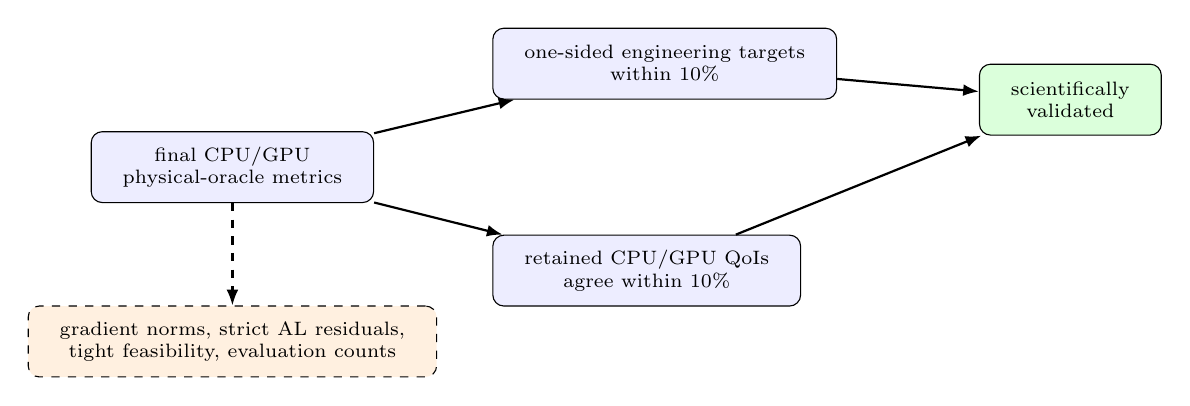
\begin{tikzpicture}[
  node distance=6mm and 10mm,
  box/.style={draw,rounded corners,align=center,minimum height=9mm,
              inner xsep=4mm,fill=blue!7,font=\scriptsize},
  pass/.style={draw,rounded corners,align=center,minimum height=9mm,
               inner xsep=4mm,fill=green!14,font=\scriptsize},
  diag/.style={draw,dashed,rounded corners,align=center,minimum height=9mm,
               inner xsep=4mm,fill=orange!12,font=\scriptsize},
  flow/.style={-{Latex[length=2mm]},thick}
]
\node[box] (oracle) {final CPU/GPU\\physical-oracle metrics};
\node[box,above right=4mm and 15mm of oracle] (target) {one-sided engineering
  targets\\within 10\%};
\node[box,below right=4mm and 15mm of oracle] (parity) {retained CPU/GPU QoIs\\
  agree within 10\%};
\node[pass,right=18mm of target.south east,anchor=west] (valid)
  {scientifically\\validated};
\node[diag,below=13mm of oracle] (diagnostics) {gradient norms, strict AL
  residuals,\\tight feasibility, evaluation counts};
\draw[flow] (oracle) -- (target);
\draw[flow] (oracle) -- (parity);
\draw[flow] (target) -- (valid);
\draw[flow] (parity) -- (valid);
\draw[flow,dashed] (oracle) -- (diagnostics);
\end{tikzpicture}
\caption{Revised validation contract.  Physical targets and CPU/GPU agreement
determine scientific validity.  First-order and strict AL checks remain visible
optimizer-health diagnostics rather than hidden or discarded signals.}
\label{fig:qoi-validation-contract}
\end{figure}

\subsection{Implemented conditioning changes}

Schema~2 implements the planned zero-preserving transform
\[
 q_\epsilon(r)=\sqrt{r^2+\epsilon^2}-\epsilon,
 \qquad q_\epsilon(0)=q_\epsilon'(0)=0,
 \qquad q_\epsilon'(r)=\frac{r}{\sqrt{r^2+\epsilon^2}}.
\]
Unlike the earlier square-root transform, this mapping neither moves the zero
set nor gives a nonzero derivative at a feasible hinge.  It is quadratic near
zero, $q_\epsilon(r)\simeq r^2/(2\epsilon)$, and approaches $r-\epsilon$ for
large positive residuals.  The Colab qualification uses
$\epsilon=0.1$ in normalized-residual coordinates to soften the boundary
region while leaving order-one violations residual-like.

Constraint scales are now dynamic inputs to the compiled CPU/GPU executable.
After an inner stage passes its absolute-or-relative first-order check and the
scaled AL progress test, each family scale follows
\[
 s_{k+1}=\max(s_{\min},\rho s_k),\qquad \rho=0.5,
 \]
with $s_{\min}=\sqrt{n_{\rm family}}$.  The multiplier is changed as
$\lambda_{k+1}\leftarrow\lambda_{k+1}s_{k+1}/s_k$, preserving the physical
linear coefficient $\lambda/s$ while the quadratic contribution is
deliberately strengthened by the smaller scale.  The gentler $\rho=0.5$
replaces the initially screened 0.25 step, which strengthened a quadratic term
by $16\times$ from scaling alone.  No JAX recompilation is needed when scales,
multipliers, or penalties change.

The inner safeguard accepts either the requested absolute threshold or a
stage-relative gradient reduction.  The production notebook asks for a
100-fold reduction.  This criterion governs whether an AL state update is safe;
it does not define scientific validity.  Every history record now retains the
initial and final infinity norms, their ratio, both thresholds, scale summaries,
and whether the update was applied.

\subsection{Retrospective classification of the measured A100 endpoints}

Applying the revised rule to the already measured engineering run changes its
scientific classification without rewriting its solver history.  Table
\ref{tab:qoi-validation-retrospective} shows that both endpoints lie comfortably
inside the 10\% physical envelope.  Across the explicitly selected CPU/GPU
quantities of interest, the largest relative difference is 1.35\% in the
objective.  The normalized-normal-field statistics differ by less than 1\%.

\begin{table}[htbp]
\centering
\caption{Retrospective 10\% target validation of the existing A100 endpoints.
The strict local-residual and stationarity failures reported earlier remain
true diagnostics, but do not invalidate these physical quantities.}
\label{tab:qoi-validation-retrospective}
\begin{tabular}{lrrl}
\toprule
Quantity & CPU & GPU & Accepted boundary \\
\midrule
Minimum coil--coil distance (m) & 0.114532 & 0.114235 & $\geq0.090$ \\
Minimum coil--surface distance (m) & 0.299875 & 0.299900 & $\geq0.270$ \\
Maximum curvature (m$^{-1}$) & 4.14766 & 4.17179 & $\leq5.50$ \\
Maximum MSC (m$^{-2}$) & 5.00100 & 5.00100 & $\leq5.50$ \\
Objective & 0.0165123 & 0.0162893 & backend difference $\leq10\%$ \\
$|B\cdot n|/|B|$ RMS & 0.191970 & 0.190910 & backend difference $\leq10\%$ \\
Total base-coil length (m) & 14.1670 & 14.1866 & backend difference $\leq10\%$ \\
\bottomrule
\end{tabular}
\end{table}

\textbf{Decision.}  The historical CPU and GPU designs are scientifically
validated under the revised 10\% quantity-of-interest criterion.  They are not
relabelled as tightly converged AL solutions: the raw local residual,
stationarity, and evaluation-budget outcomes remain failed diagnostics.  The
next A100 run will test the new smoothed scale continuation and emit both
\code{scientifically\_validated} and the separate technical/performance gates,
along with the mandatory final JSON metrics, surface VTS files carrying
$B\cdot n/|B|$, and coil VTU files.

\subsection{Measured smoothed-continuation A100 run}

The schema-2 archive was returned from commit \code{9859d577} with SHA-256
prefix \code{397b14a264372498}.  It contains the result JSON and nonempty CPU
and GPU surface VTS and coil VTU files.  The run used an NVIDIA A100-SXM4-40GB,
JAX 0.11.1 in float64, SciPy 1.16.3, $\epsilon=0.1$, $\rho=0.5$, eight allowed
outer stages, and 300 inner iterations per stage.  Its initial CPU/GPU base
objective, residual vector, and gradient agree respectively to
$6.94\times10^{-18}$ absolute, $1.20\times10^{-16}$ relative, and
$1.14\times10^{-16}$ relative error.  The numerical kernels therefore remain
qualified at the common initial state.

The two optimizations nevertheless separate during the first inner solve.
SciPy requires 121 CPU iterations and 333 evaluations but only 24 GPU
iterations and 104 evaluations before each endpoint satisfies the deliberately
loose first-stage criterion.  Their base objectives are already 0.0143662 and
0.0164681.  Both then accept the AL update and halve the coil--surface scale
from 18,498.1 to 9,249.0.  The second inner solves exhaust 300 iterations; the
CPU and GPU gradient infinity norms increase to 182.75 and 49.21, so the
safeguard correctly prevents another AL state update.  Large gradients remain
diagnostic rather than a scientific veto, but this history identifies the
point at which the two nonconvex trajectories diverge.

\begin{figure}[htbp]
\centering
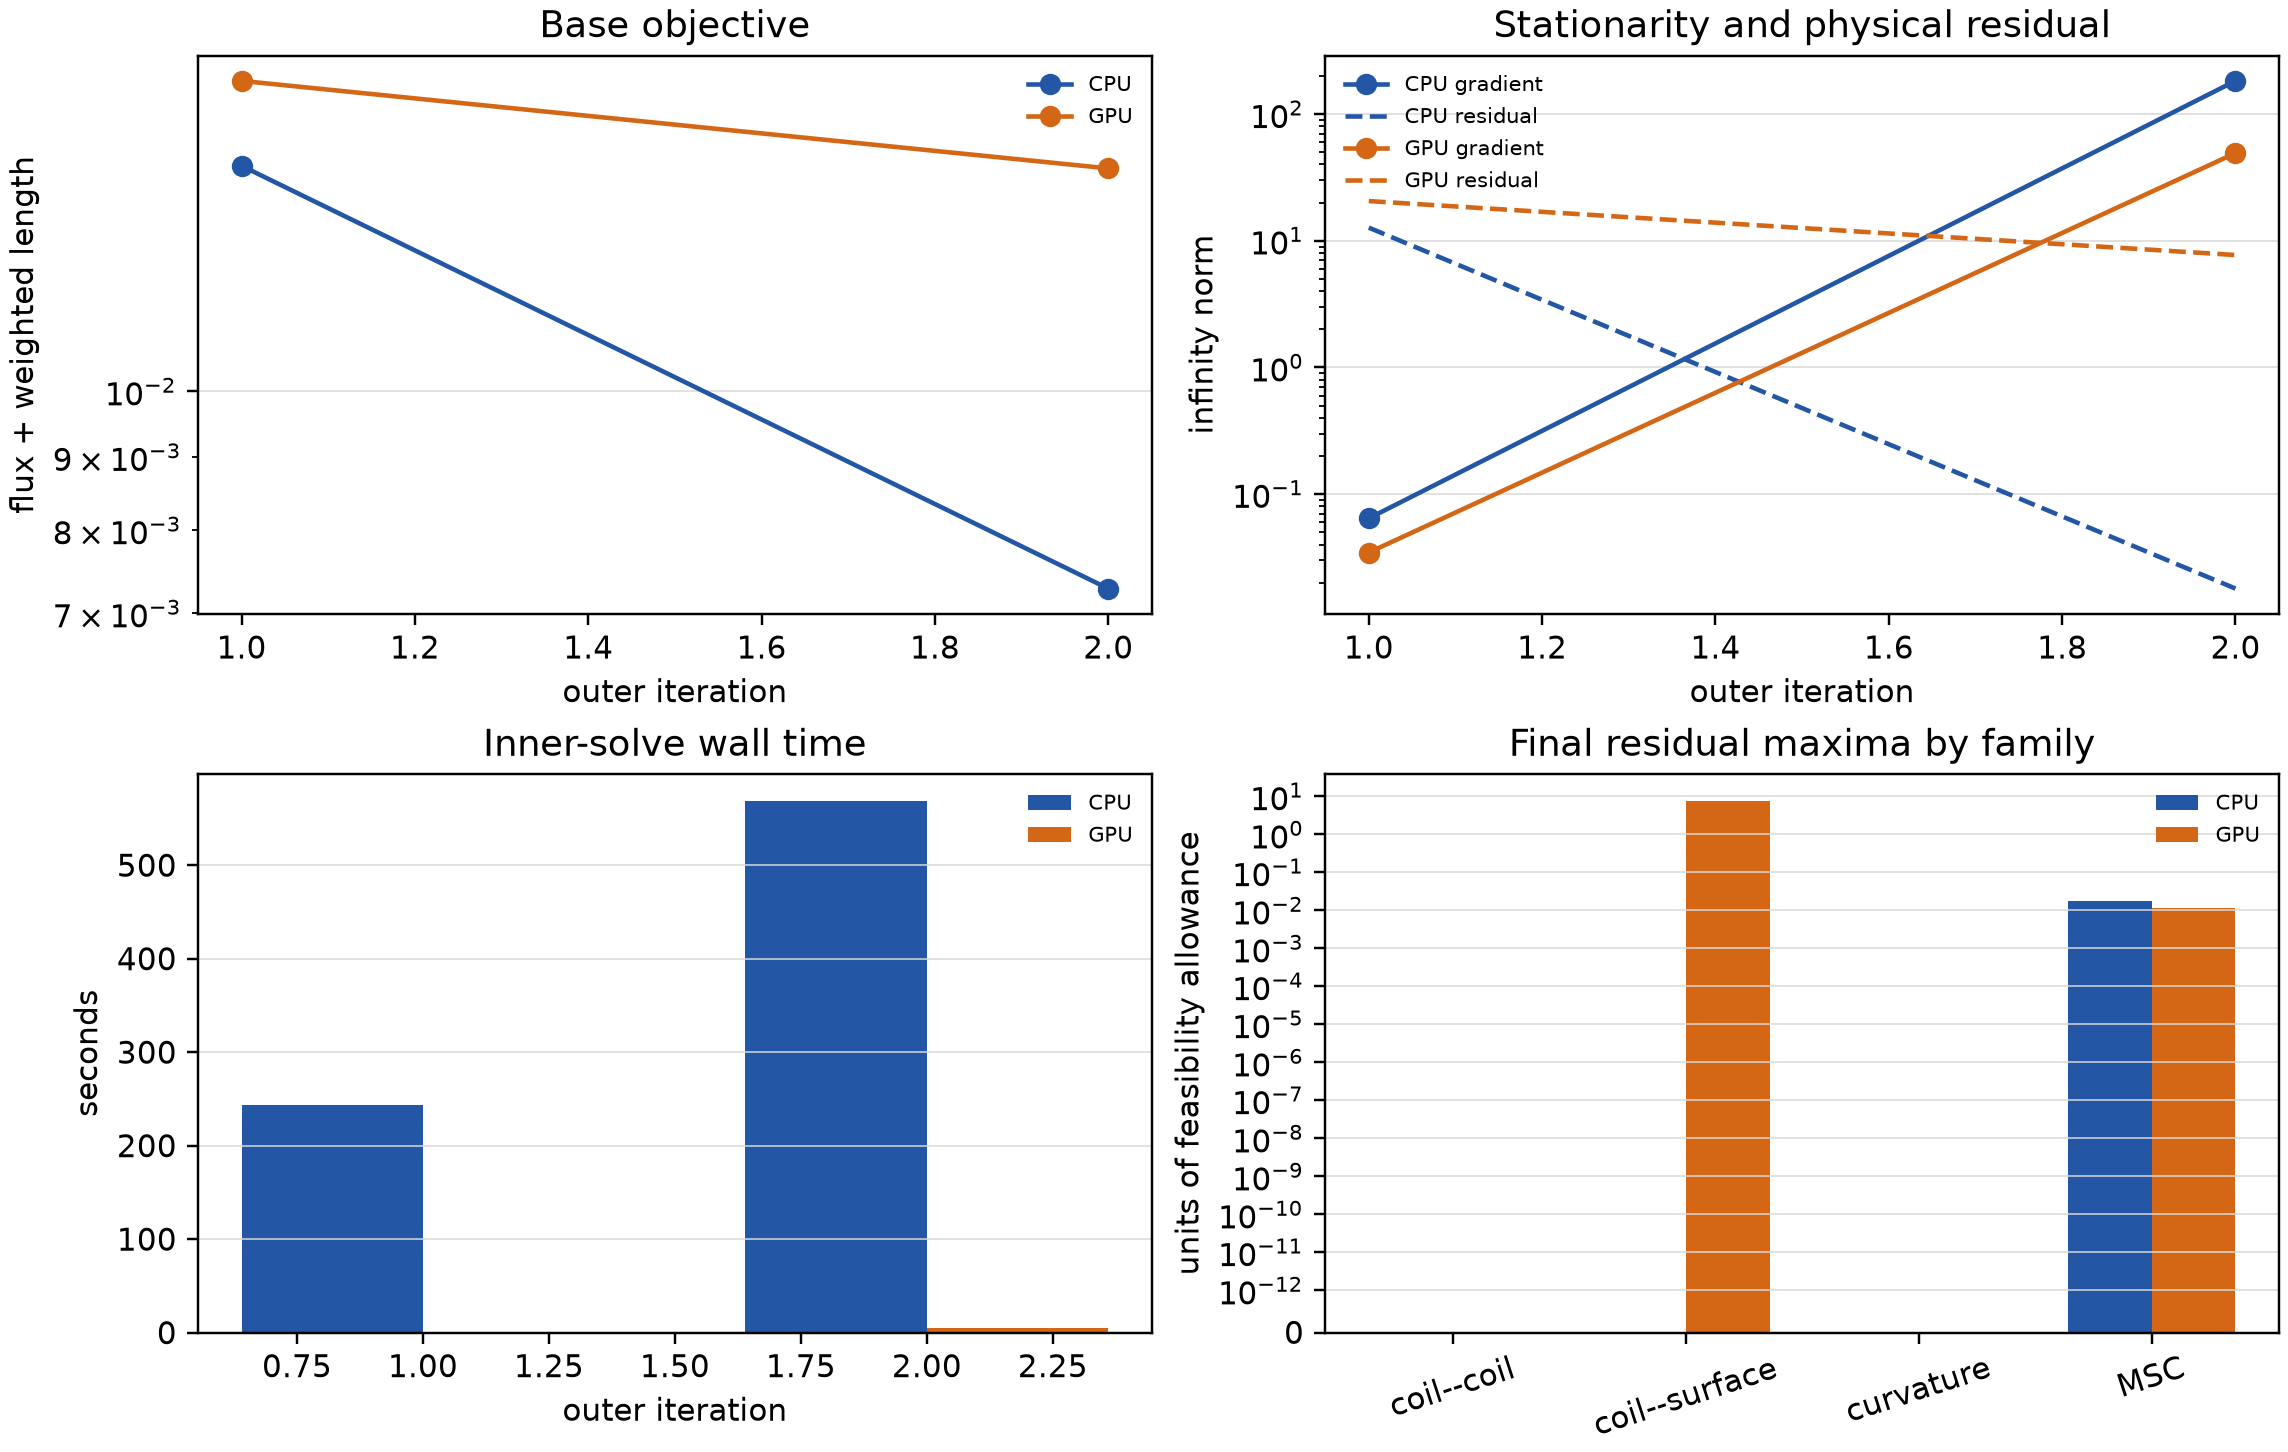
\includegraphics[width=\textwidth]{figures/smoothed_local_residual_al_convergence.png}
\caption{Measured schema-2 optimization histories.  Both backends accept the
first smoothed-continuation stage.  The CPU obtains a substantially lower base
objective in stage two, while both gradients grow and both strict residual
diagnostics remain nonzero.}
\label{fig:smoothed-local-residual-al-convergence}
\end{figure}

Table~\ref{tab:smoothed-local-residual-al-result} separates target satisfaction
from cross-backend agreement.  Every direct engineering measurement for both
designs lies within its one-sided 10\% target envelope.  Total base-coil length
and coil--surface distance also agree within 10\%.  Scientific validation still
fails because the GPU objective is 96.44\% above the CPU reference and the
three normalized-normal-field statistics differ by 33.92--37.38\%.  The
coil--coil and maximum-curvature measurements differ by 18.20\% and 12.34\%,
respectively, although both are on the acceptable side of their direct physical
targets.  This distinction prevents a better-than-limit constraint value from
being mistaken for physical infeasibility.

\begin{table}[htbp]
\centering
\caption{Final schema-2 quantities of interest.  ``Target'' applies the
one-sided physical engineering envelope; ``agreement'' compares the GPU
endpoint with the CPU reference.}
\label{tab:smoothed-local-residual-al-result}
\begin{tabular}{lrrrl}
\toprule
Quantity & CPU & GPU & Difference & Result \\
\midrule
Objective & 0.00728381 & 0.0143083 & 96.44\% & fail agreement \\
$|B\cdot n|/|B|$ mean & 0.112602 & 0.154691 & 37.38\% & fail agreement \\
$|B\cdot n|/|B|$ RMS & 0.135023 & 0.180828 & 33.92\% & fail agreement \\
$|B\cdot n|/|B|$ maximum & 0.264221 & 0.359019 & 35.88\% & fail agreement \\
Total base-coil length (m) & 14.9170 & 14.2020 & 4.79\% & pass agreement \\
Minimum coil--coil distance (m) & 0.144847 & 0.118481 & 18.20\% & pass target \\
Minimum coil--surface distance (m) & 0.302014 & 0.299129 & 0.96\% & pass target \\
Maximum curvature (m$^{-1}$) & 5.00099 & 4.38381 & 12.34\% & pass target \\
Maximum MSC (m$^{-2}$) & 5.00102 & 5.00101 & $1.3\times10^{-4}$\% & pass target \\
\bottomrule
\end{tabular}
\end{table}

\begin{figure}[htbp]
\centering
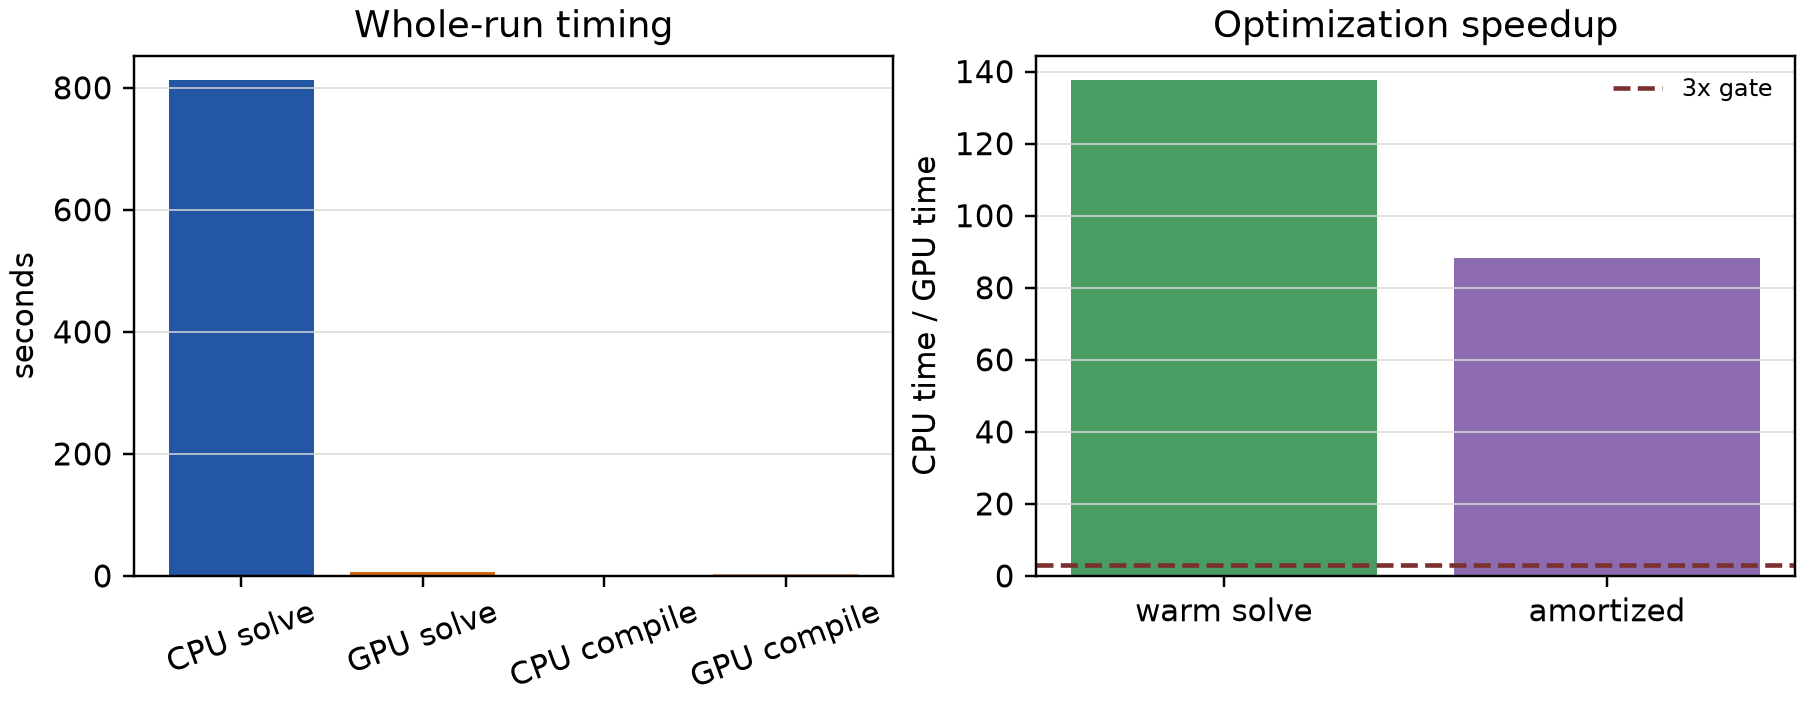
\includegraphics[width=0.92\textwidth]{figures/smoothed_local_residual_al_performance.png}
\caption{A100 timing for the schema-2 run.  CPU and GPU solve times are
812.27~s and 5.904~s, giving $137.58\times$ warm speedup and $88.12\times$
speedup including 3.314~s GPU compilation.  The result is a throughput
measurement because the endpoint QoIs do not agree.}
\label{fig:smoothed-local-residual-al-performance}
\end{figure}

The exported signed surface fields have correlation 0.98660, relative
$L^2$ difference 0.38931, and maximum pointwise difference 0.10978.  The maps
retain the same broad structure but show a materially stronger GPU normal-field
error, consistent with the scalar metrics.

\begin{figure}[htbp]
\centering
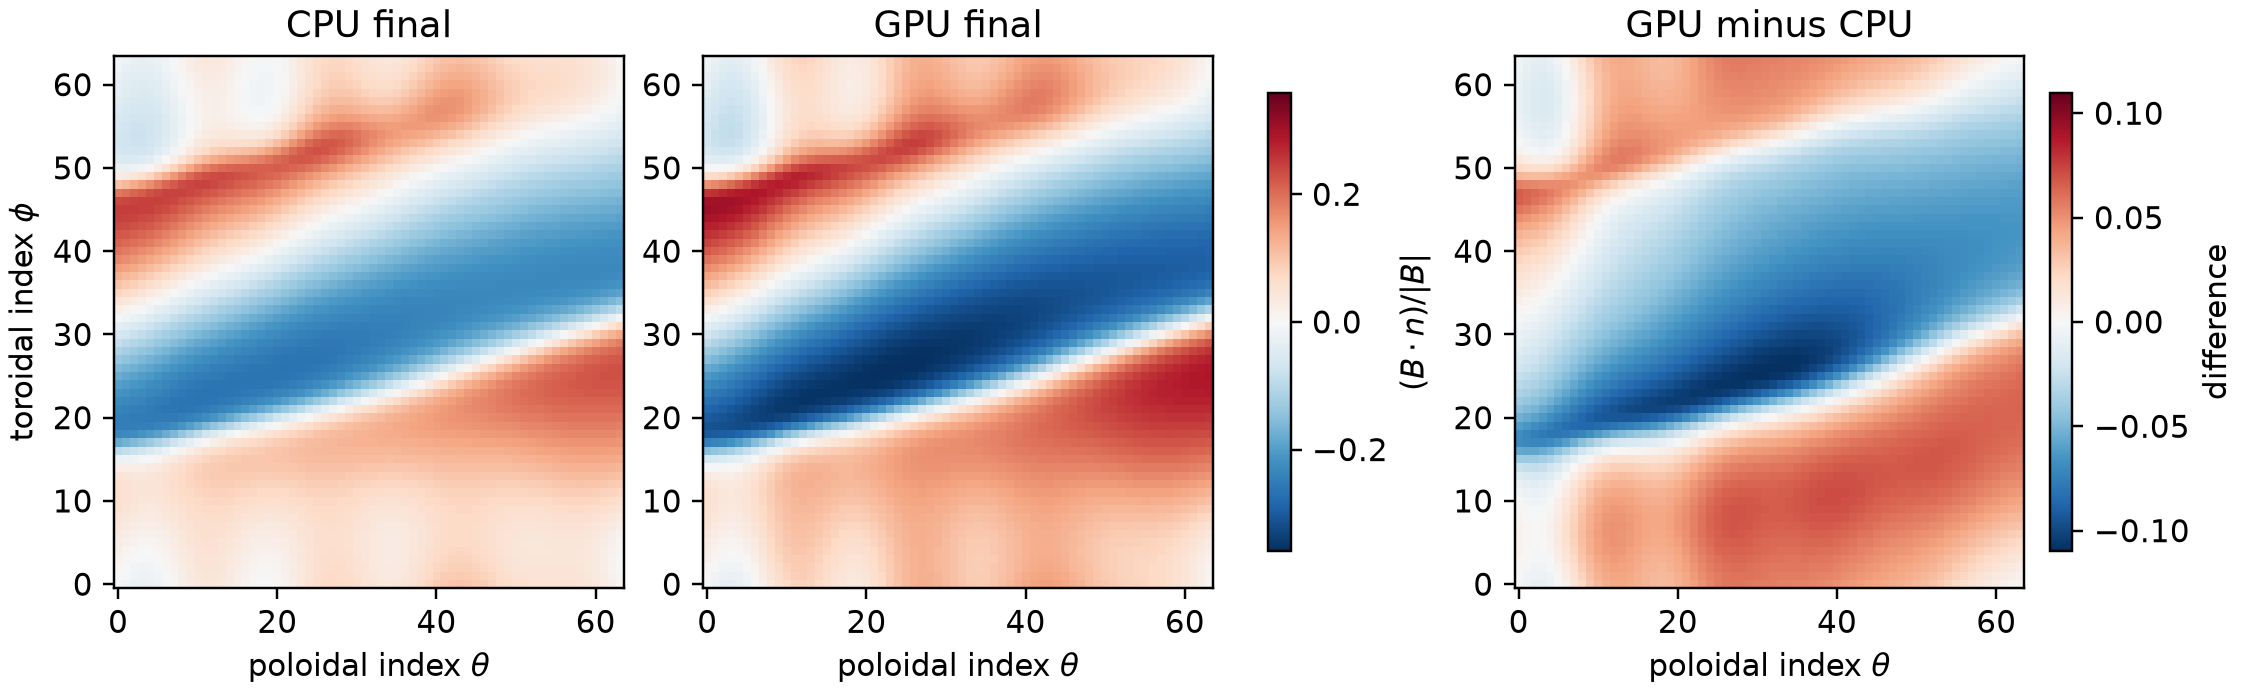
\includegraphics[width=\textwidth]{figures/smoothed_local_residual_al_surface.png}
\caption{Signed $(B\cdot n)/|B|$ data read back from the exported VTS files.
The spatial difference is coherent rather than isolated roundoff, confirming
that independently stopped L-BFGS-B trajectories reached different designs.}
\label{fig:smoothed-local-residual-al-surface}
\end{figure}

\textbf{Decision.}  Accept the archive, VTK contract, initial numerical parity,
all direct 10\% engineering targets, the evaluation-budget diagnostic (784 GPU
versus 1,114 CPU evaluations), and the A100 throughput result.  Reject
scientific validation and any equivalent-solution speedup claim because the
objective and normalized-normal-field QoIs fail the 10\% reference envelope.
Do not tune $\epsilon$ or $\rho$ next: the evidence points first to optimizer
trajectory control.  The next implementation should separate three contracts:
(i) same-point CPU/GPU objective and gradient parity, (ii) scientific quality of
each physical design against explicit targets, and (iii) optimizer performance.
For independent nonconvex solves it should retain the best target-feasible
checkpoint and compare quality at a matched evaluation budget, while a locked
GPU trajectory is replayed through the CPU oracle to validate the final design
without incorrectly requiring two floating-point line searches to follow the
same basin.

\section{Target-feasible quadratic-flux refinement}

The preceding decision did not yet impose the required absolute magnetic
quality.  The CPU and GPU \emph{quadratic-flux components} in the schema-2
archive are $7.26889\times10^{-3}$ and $1.42941\times10^{-2}$, respectively.
Those are approximately $727\times$ and $1{,}429\times$ the new production
target $J_{\rm QF}=10^{-5}$.  Agreement with another poor endpoint would not
make either design acceptable.  Schema 3 therefore replaces cross-backend
quantity agreement in the scientific rule with the explicit one-sided test
\[
 J_{\rm QF}\leq (1+\delta)10^{-5}=1.1\times10^{-5},\qquad \delta=0.10,
\]
while retaining CPU/GPU agreement as a separate technical diagnostic.  This
target requires roughly three orders of magnitude of improvement from the
measured endpoints.  Large gradients continue to be recorded but cannot veto
or confer scientific validity.

\begin{figure}[htbp]
\centering
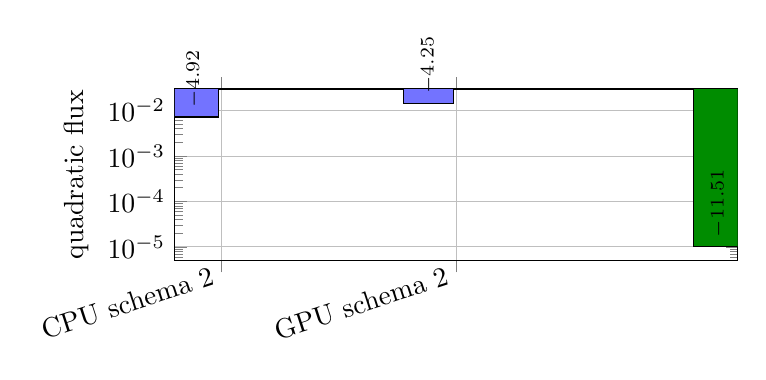
\begin{tikzpicture}
\begin{axis}[
  ybar,ymode=log,width=0.72\textwidth,height=0.31\textwidth,
  ymin=5e-6,ymax=3e-2,
  ylabel={quadratic flux},
  symbolic x coords={CPU schema 2,GPU schema 2,production target},
  xtick=data,x tick label style={rotate=18,anchor=east},
  nodes near coords,nodes near coords style={font=\scriptsize,rotate=90,anchor=west},
  grid=major,bar width=18pt]
\addplot[fill=blue!55] coordinates {
  (CPU schema 2,0.0072688939894)
  (GPU schema 2,0.0142940658131)
};
\addplot[fill=green!55!black] coordinates {(production target,0.00001)};
\end{axis}
\end{tikzpicture}
\caption{The missing absolute quality criterion.  The schema-2 quadratic flux,
not merely its CPU/GPU difference, is about three orders of magnitude above the
required production level.  The schema-3 pass boundary includes the agreed
10\% allowance and is $1.1\times10^{-5}$.}
\label{fig:quadratic-flux-gap}
\end{figure}

\subsection{Implemented two-phase algorithm}

The local-residual AL is retained only as a mechanism for obtaining candidate
feasibility warm starts.  Both AL endpoints are evaluated by one compiled
quality program.  The lower-flux endpoint is selected if it satisfies every
10\% engineering envelope; otherwise selection minimizes target-envelope
residual first and flux second.  Both CPU and GPU refinements then start from
this \emph{same} vector.  This removes the known initial-basin mismatch from the
timed refinement comparison and isolates execution-device differences.

The refinement objective is the complete GPU-native direct objective:
quadratic flux, the small length regularizer, coil--coil and coil--surface
distance penalties, curvature, and mean-squared curvature.  Its hinge
boundaries are moved to the accepted physical envelope,
\[
 d_{cc}\geq0.09\ {\rm m},\quad d_{cs}\geq0.27\ {\rm m},\quad
 \kappa_{\max}\leq5.5\ {\rm m}^{-1},\quad {\rm MSC}_{\max}\leq5.5\ {\rm m}^{-2}.
\]
This gives the optimizer room to trade unused engineering margin for magnetic
quality without weakening the scientific contract.  L-BFGS-B is allowed 600
iterations and 1,500 value--gradient evaluations on each backend.

\begin{figure}[htbp]
\centering
\resizebox{\textwidth}{!}{%
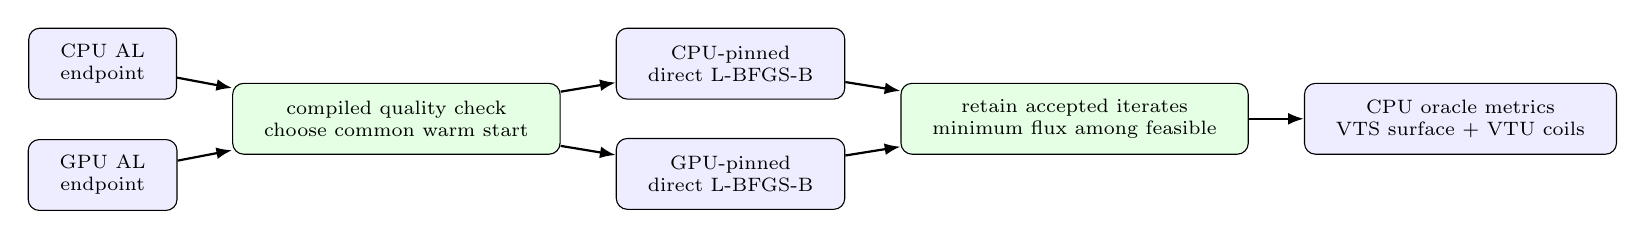
\begin{tikzpicture}[
  node distance=5mm and 7mm,
  box/.style={draw,rounded corners,align=center,minimum height=9mm,
              inner xsep=4mm,fill=blue!7,font=\scriptsize},
  check/.style={draw,rounded corners,align=center,minimum height=9mm,
                inner xsep=4mm,fill=green!10,font=\scriptsize},
  flow/.style={-{Latex[length=2mm]},thick}
]
\node[box] (cpu-al) {CPU AL\\endpoint};
\node[box,below=of cpu-al] (gpu-al) {GPU AL\\endpoint};
\node[check,right=of cpu-al,yshift=-7mm] (rank) {compiled quality check\\choose common warm start};
\node[box,right=of rank,yshift=7mm] (cpu-ref) {CPU-pinned\\direct L-BFGS-B};
\node[box,right=of rank,yshift=-7mm] (gpu-ref) {GPU-pinned\\direct L-BFGS-B};
\node[check,right=of cpu-ref,yshift=-7mm] (checkpoint) {retain accepted iterates\\minimum flux among feasible};
\node[box,right=of checkpoint] (artifacts) {CPU oracle metrics\\VTS surface + VTU coils};
\draw[flow] (cpu-al) -- (rank);
\draw[flow] (gpu-al) -- (rank);
\draw[flow] (rank) -- (cpu-ref);
\draw[flow] (rank) -- (gpu-ref);
\draw[flow] (cpu-ref) -- (checkpoint);
\draw[flow] (gpu-ref) -- (checkpoint);
\draw[flow] (checkpoint) -- (artifacts);
\end{tikzpicture}
}
\caption{Schema-3 optimization and validation flow.  The common warm start
makes the device comparison matched.  Best-feasible checkpointing prevents a
late infeasible line-search step from replacing an earlier scientifically
better state.}
\label{fig:flux-refinement-flow}
\end{figure}

Every accepted refinement iterate is assessed with local residuals whose zero
set exactly matches the 10\% target envelope.  The final state is the minimum
quadratic-flux feasible checkpoint, not automatically SciPy's terminal state.
If no accepted state is target-feasible, the least-infeasible state is exported
for diagnosis and scientific validation fails.  Thus artifact production is
never suppressed by failure.  The result schema records all compact checkpoint
metrics, phase-specific iteration/evaluation counts and times, compilation
times, AL and refinement speedups, the final independent CPU-oracle quantities,
and the mandatory VTS/VTU files.

Explicit device selection was added to the generic SciPy objective bridge.
The CPU and GPU direct objectives are now lowered to requested JAX devices in
one process, matching the existing augmented-Lagrangian bridge behavior.  A
new analysis figure will plot accepted-checkpoint quadratic flux, distinguish
target-feasible points, draw the $1.1\times10^{-5}$ boundary, and mark the
exported checkpoint once the next A100 archive is returned.  No performance or
convergence claim is made before that measurement.

\textbf{Decision.}  Run the schema-3 Colab qualification with
\code{--quadratic-flux-target 1e-5}.  Scientific success requires both exported
designs to pass that flux target and all four engineering envelopes.  CPU/GPU
QoI agreement, first-order convergence, strict AL residuals, and speedup remain
visible, independent gates or diagnostics.  The next decision will be based on
the returned JSON and the spatial $B\cdot n/|B|$ fields, not optimizer status
alone.

\paragraph{Notebook validation correction.}
The first schema-3 Colab run completed its optimization but stopped in the
artifact-validation cell because the notebook compared
\code{target\_allowed\_boundary} with $1.1\times10^{-5}$ using exact
floating-point equality.  The stored value is computed as
$10^{-5}(1+0.10)$ and can differ from the decimal literal by one binary
rounding unit.  This is a test-harness defect, not a numerical or optimization
failure.  The assertion now uses \code{math.isclose} with relative tolerance
$10^{-14}$ and zero absolute tolerance; the result JSON and previously
generated VTK artifacts require no repair.

\subsection{Measured schema-3 A100 qualification}

The returned schema-3 archive has SHA-256
\code{284c392276e0d0ac\allowbreak{}5729a67e55c626d0\allowbreak{}%
7b76b49950a9443d\allowbreak{}b13fdc32cbcf5f50}
and was produced from commit \code{cf21da23}.  It contains the result JSON and
four nonempty visualization files: CPU/GPU surfaces in VTS format and
CPU/GPU symmetry-expanded coils in VTU format.  The surface files contain
signed and absolute $B\cdot n/|B|$, $B\cdot n$, and $|B|$.  The run used an
NVIDIA A100-SXM4-40GB, JAX 0.11.1 in float64, SciPy 1.16.3, and the schema-3
settings specified above.

The common-warm-start policy selected the CPU AL endpoint because both
candidates were target-feasible and its quadratic flux,
$7.26889\times10^{-3}$, was lower than the GPU candidate's
$1.58035\times10^{-2}$.  Starting from that identical vector, both direct
refinements select accepted checkpoint 44.  The independent SIMSOPT CPU oracle
measures quadratic flux $8.61564\times10^{-7}$ for both designs.  This is
$11.61\times$ below the nominal $10^{-5}$ target, $12.77\times$ below the
allowed $1.1\times10^{-5}$ boundary, and $8{,}437\times$ below the preceding
CPU endpoint.  The requested three-order reduction is therefore exceeded.

\begin{table}[htbp]
\centering
\caption{Final schema-3 quantities measured by the independent SIMSOPT CPU
oracle.  Both designs pass every one-sided 10\% engineering envelope and the
explicit quadratic-flux target.}
\label{tab:flux-refinement-result}
\begin{tabular}{lrrl}
\toprule
Quantity & CPU & GPU & Scientific boundary \\
\midrule
Quadratic flux & $8.615638\times10^{-7}$ & $8.615638\times10^{-7}$
  & $\leq1.1\times10^{-5}$ \\
$|B\cdot n|/|B|$ mean & 0.00135658 & 0.00135658 & retained QoI \\
$|B\cdot n|/|B|$ RMS & 0.00174133 & 0.00174133 & retained QoI \\
$|B\cdot n|/|B|$ maximum & 0.00611851 & 0.00611851 & retained QoI \\
Minimum coil--coil distance (m) & 0.139627 & 0.139627 & $\geq0.090$ \\
Minimum coil--surface distance (m) & 0.280193 & 0.280193 & $\geq0.270$ \\
Maximum curvature (m$^{-1}$) & 5.03888 & 5.03888 & $\leq5.50$ \\
Maximum MSC (m$^{-2}$) & 5.47919 & 5.47919 & $\leq5.50$ \\
Total base-coil length (m) & 17.8202 & 17.8202 & retained QoI \\
\bottomrule
\end{tabular}
\end{table}

The CPU/GPU match is much stronger than the required 10\%.  Quadratic flux
differs by $7.0\times10^{-11}$ relatively; normalized-normal-field statistics
by at most $7.9\times10^{-11}$; engineering measurements by at most
$3.9\times10^{-9}$; and the largest relative difference anywhere in the
flattened oracle metrics is $1.12\times10^{-6}$, arising in a very small
curvature-penalty component.  All six acceptance gates pass and
\code{scientifically\_validated} is true.

\begin{figure}[htbp]
\centering
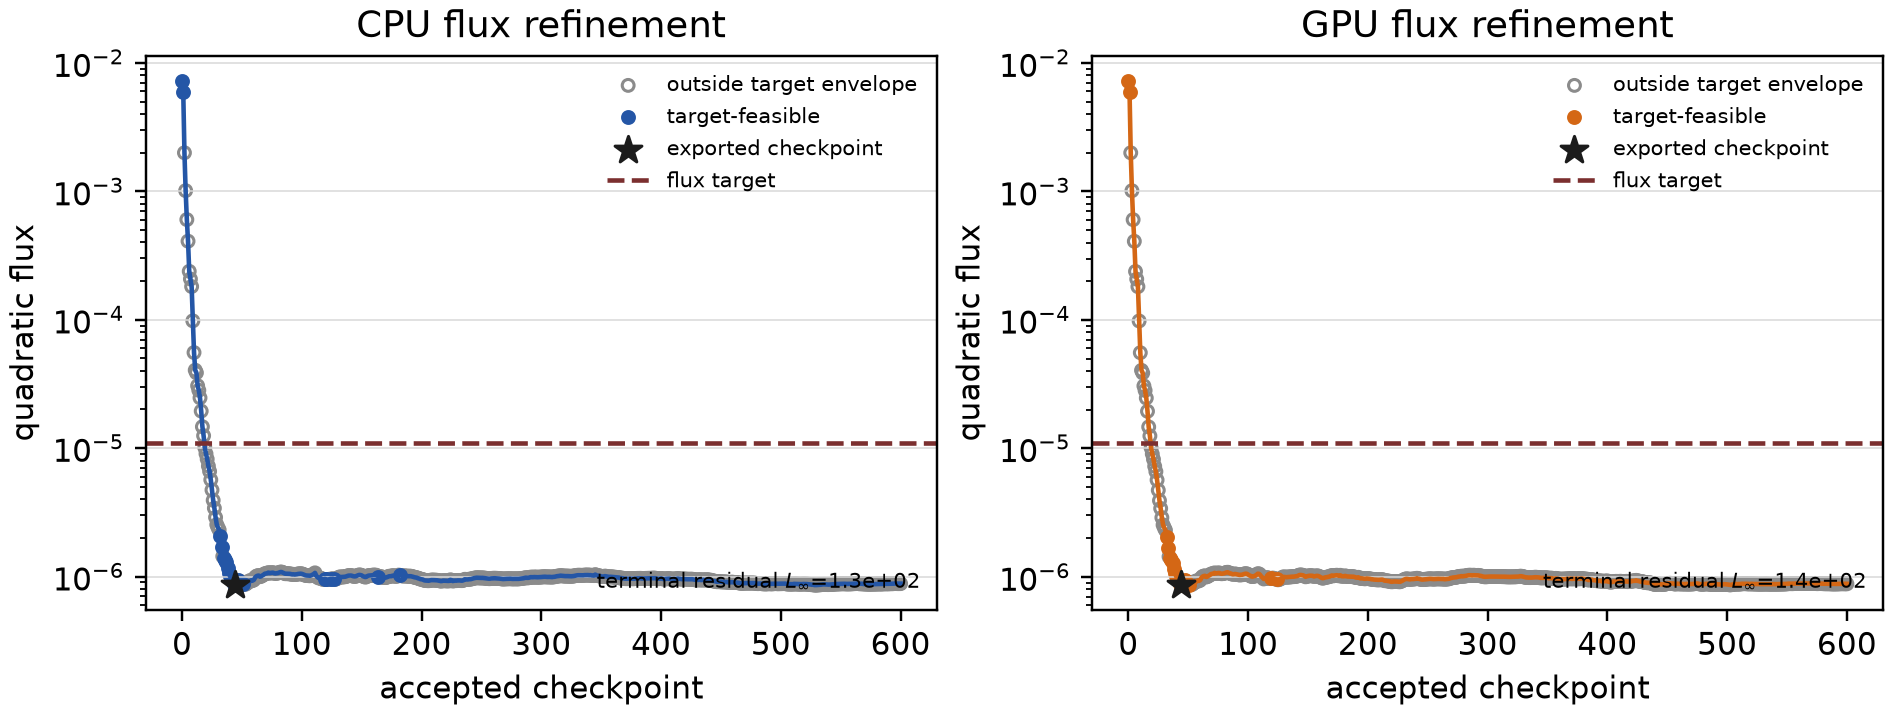
\includegraphics[width=\textwidth]{figures/flux_target_refinement_trajectory.png}
\caption{Accepted-checkpoint quadratic flux for the matched CPU and GPU
refinements.  Filled markers satisfy every engineering target envelope; open
markers do not.  Both backends select checkpoint 44 (star) at
$8.61564\times10^{-7}$.  Later iterates remain low-flux but leave the allowed
engineering envelope, demonstrating why terminal-state export would be
incorrect.}
\label{fig:flux-target-refinement-trajectory}
\end{figure}

Both L-BFGS-B refinements reach their 600-iteration cap rather than report
stationary convergence.  The CPU retains 22 feasible candidates and the GPU
18; their selected checkpoint is nevertheless the same physical design to
roundoff.  At iteration 600 the target-envelope residual infinity norms are
128.98 and 135.46, so those terminal states are correctly rejected.  This
provides direct experimental validation of best-feasible checkpointing.  It
also shows that optimizer success flags and terminal gradients cannot replace
physical target evaluation in this nonconvex problem.

\begin{figure}[htbp]
\centering
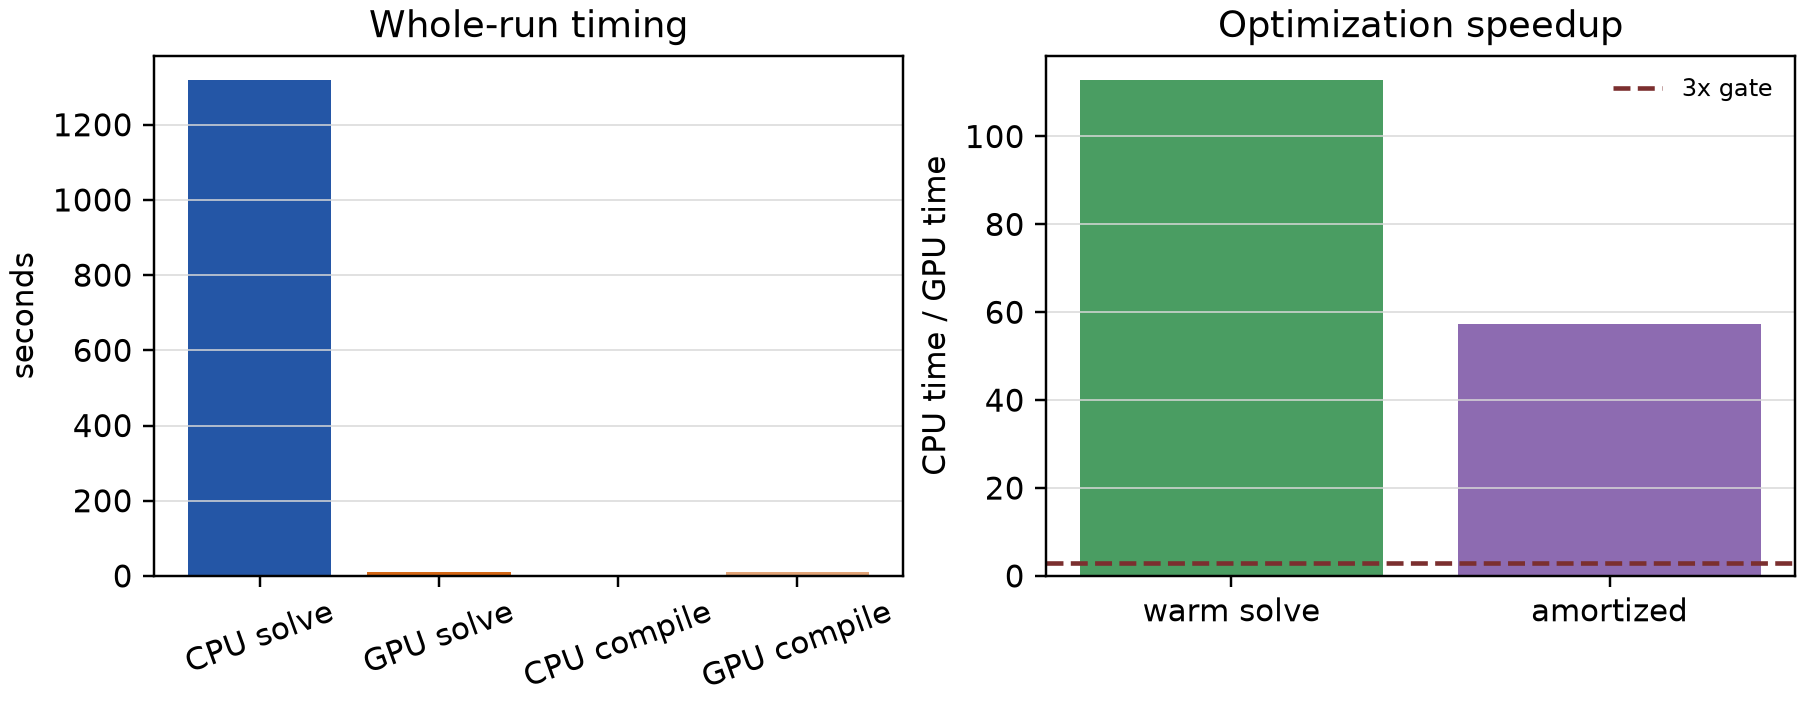
\includegraphics[width=0.94\textwidth]{figures/flux_target_refinement_performance.png}
\caption{Schema-3 A100 timing.  The combined AL and refinement phases require
1,318.25~s on CPU and 11.688~s on GPU, giving $112.78\times$ warm end-to-end
speedup.  Including all GPU compilation and quality-program costs leaves
$57.37\times$ amortized speedup.}
\label{fig:flux-target-refinement-performance}
\end{figure}

Phase-specific speedups are $142.89\times$ for AL and $83.98\times$ for direct
refinement.  CPU AL/refinement times are 816.56/501.69~s; GPU times are
5.715/5.974~s.  GPU compilation takes 3.545~s for AL, 5.555~s for refinement,
and 2.190~s for the checkpoint-quality program.  The GPU performs 752 AL and
761 refinement evaluations, compared with 1,114 and 754 on CPU.  Because the
reported designs meet the same absolute targets and agree numerically, these
are now valid equivalent-quality speedups rather than throughput-only figures.

\begin{figure}[htbp]
\centering
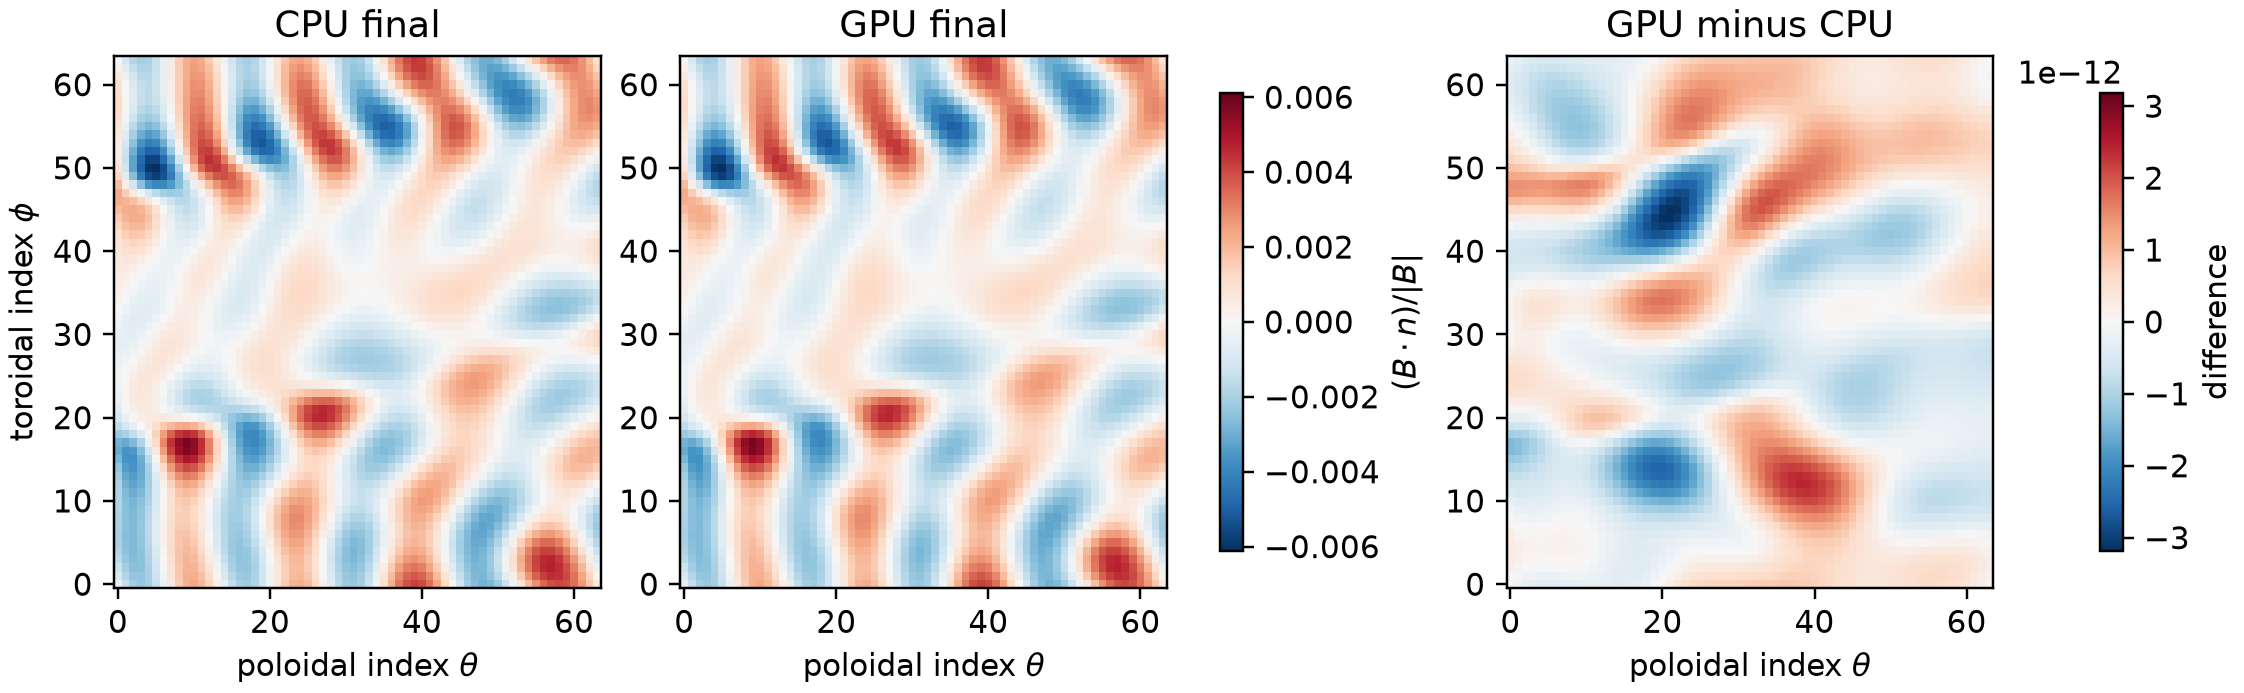
\includegraphics[width=\textwidth]{figures/flux_target_refinement_surface.png}
\caption{Signed $(B\cdot n)/|B|$ read from the exported schema-3 surface VTS
files.  The fields have correlation 1.0, relative $L^2$ difference
$4.88\times10^{-10}$, and maximum pointwise difference
$3.19\times10^{-12}$.}
\label{fig:flux-target-refinement-surface}
\end{figure}

The normalized-normal-field RMS falls from 0.1350/0.1808 in the preceding
independent CPU/GPU endpoints to 0.001741 in the matched refined design,
improvements of approximately $77.5\times$ and $103.8\times$.  The surface
maps confirm that this improvement is spatially consistent rather than a
scalar-reporting artifact.

\begin{figure}[htbp]
\centering
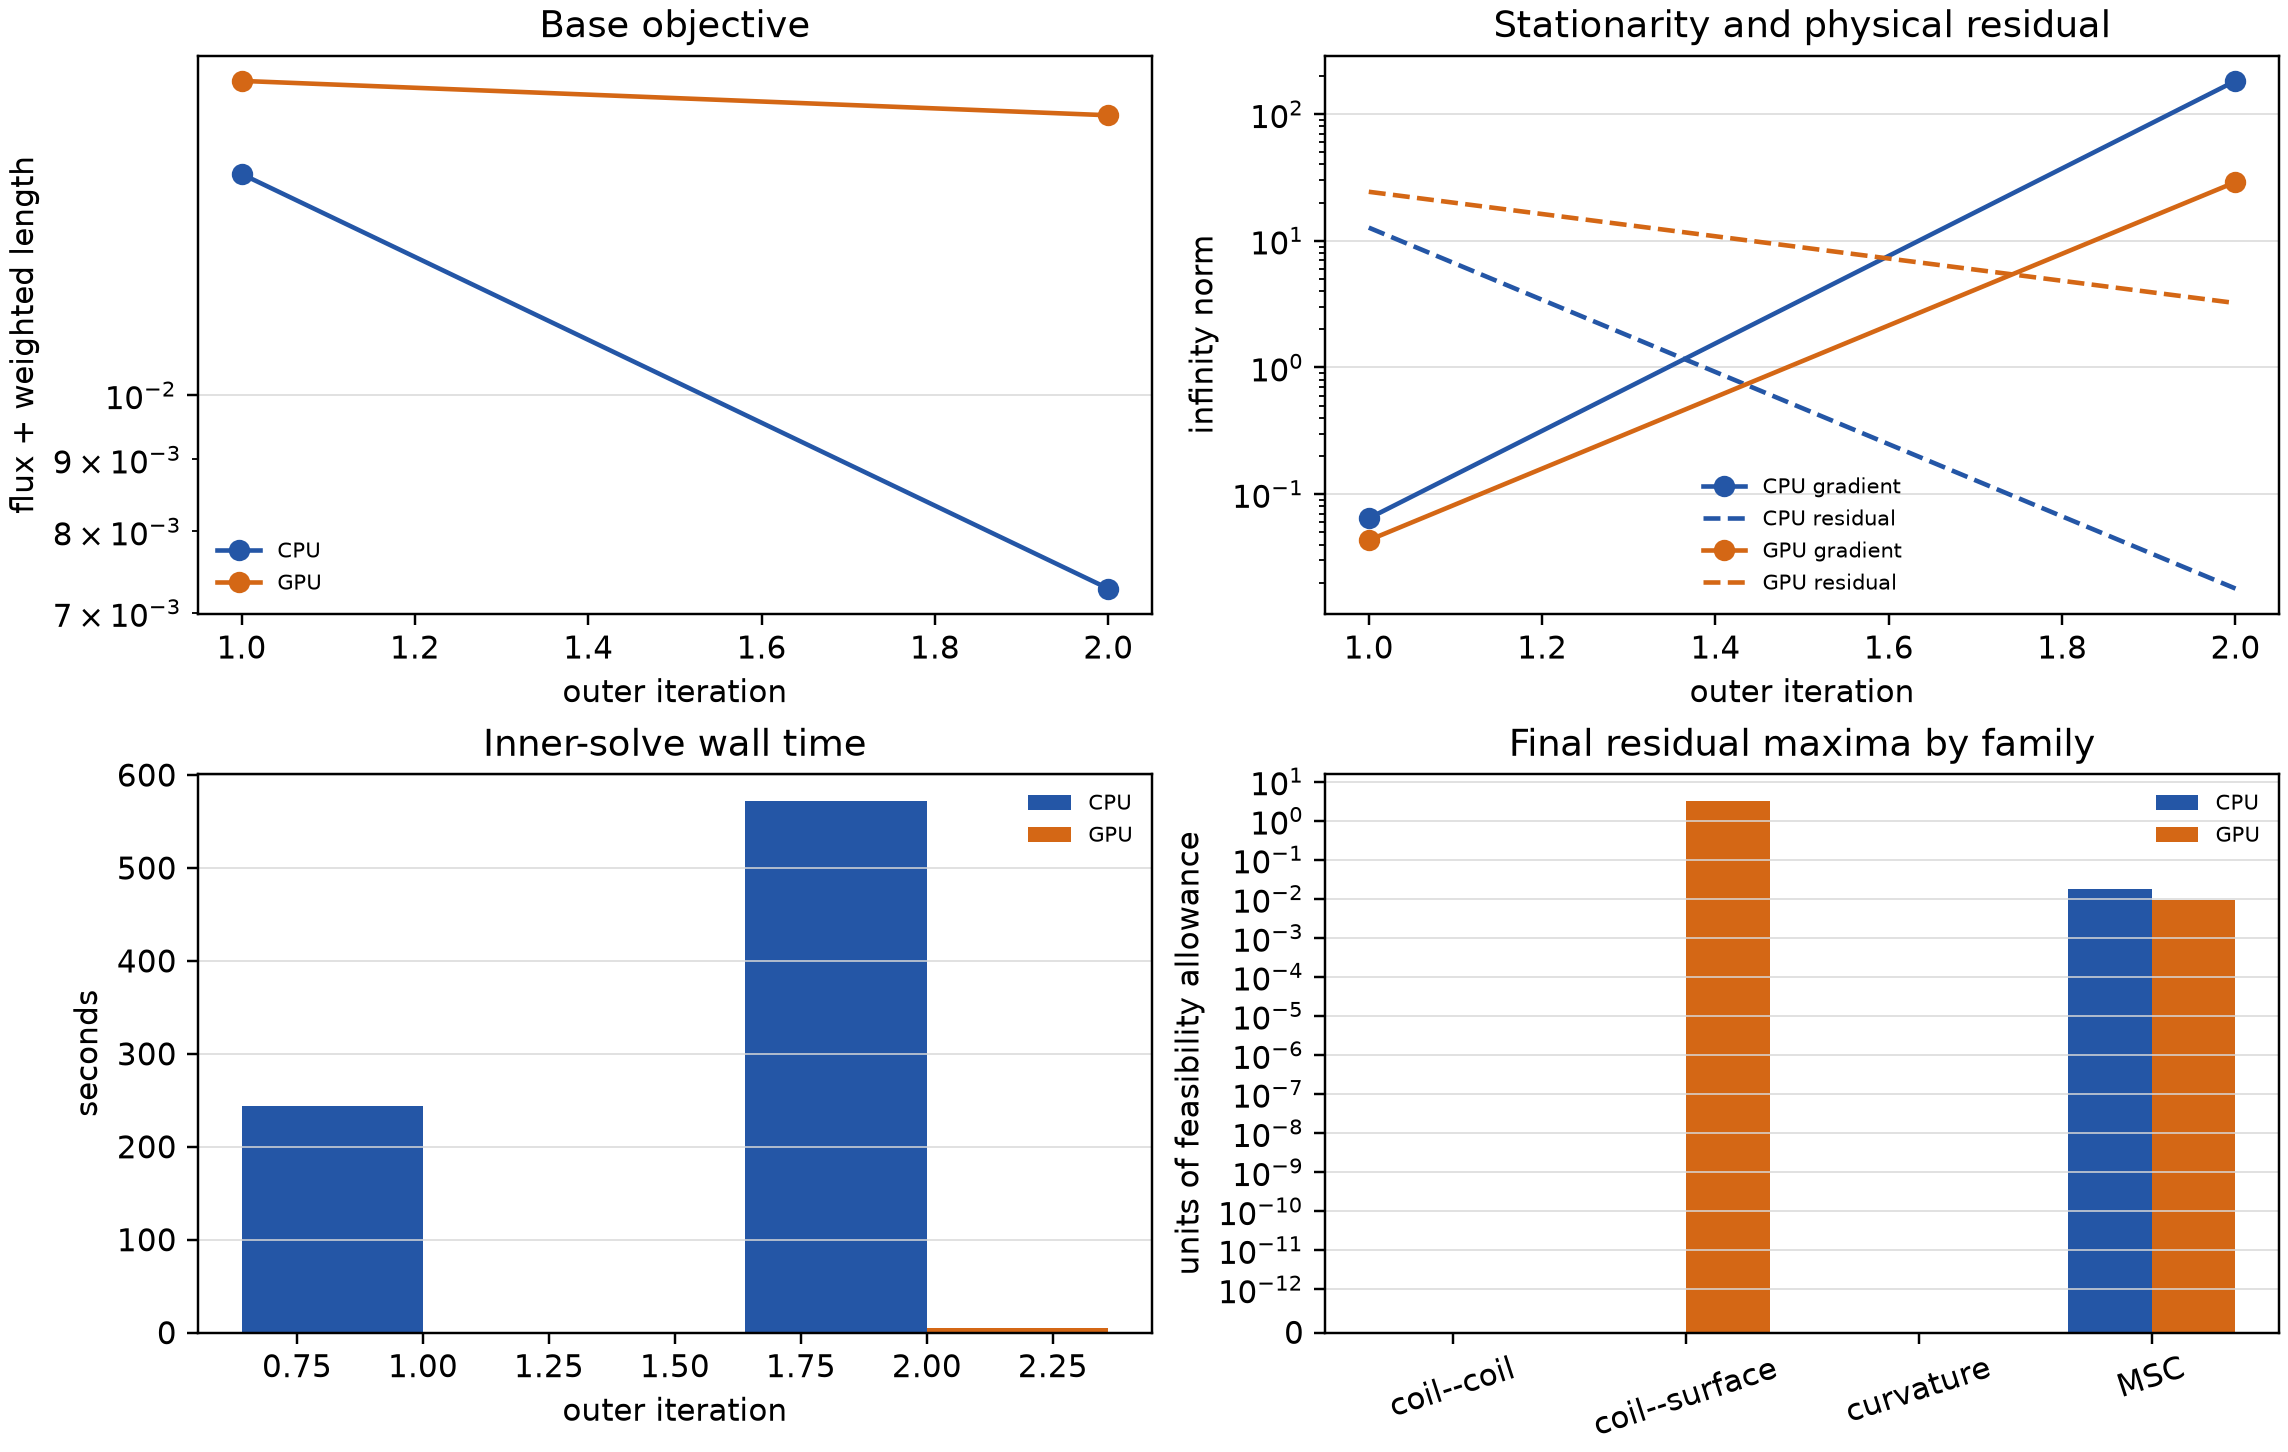
\includegraphics[width=0.94\textwidth]{figures/flux_target_refinement_convergence.png}
\caption{The retained AL warm-start diagnostics.  Strict original-threshold
residual and first-order tests remain failed, as expected, but do not affect
the subsequent target-envelope refinement or its independently measured
scientific result.}
\label{fig:flux-target-refinement-al}
\end{figure}

\textbf{Decision.}  Promote the GPU-native direct coil objective, its float64
gradient, matched-start SciPy bridge, target-envelope validation, and VTK
artifact contract as scientifically and numerically qualified on the
engineering problem.  Accept the measured $112.78\times$ warm and
$57.37\times$ amortized end-to-end speedups.  Retain AL stationarity and strict
original-threshold violations only as diagnostics: the explicit project rule
permits 10\% target deviation, and every actual quantity of interest passes.
For the next implementation, avoid spending hundreds of iterations after the
best feasible design has already been found: add target-aware feasible
checkpoint patience and then compare that reduced host-driven baseline with a
device-resident L-BFGS implementation.  The production criterion remains the
same independent CPU-oracle metrics, not the solver status.

\section{Target-aware and fully device-resident L-BFGS}

The next implementation is now complete in code and emits schema~4.  It makes
two controlled changes while retaining the schema-3 physical contract.  First,
both SciPy L-BFGS-B baselines stop when further accepted iterates no longer add
useful target-feasible information.  Second, a new JAX L-BFGS implementation
places the optimizer state transition itself on the accelerator.  The three
refinements use the same physical warm start, float64 direct objective,
target-envelope residual oracle, quadratic-flux boundary, and final checkpoint
selection.  This design separates the effect of target-aware stopping from the
effect of removing Python and SciPy from the iteration loop.

\subsection{Target-aware accepted-checkpoint policy}

Let $F_k$ be quadratic flux and $r_k$ the infinity norm of the four-family
engineering target-envelope residual at accepted checkpoint $k$.  A checkpoint
is engineering-feasible when $r_k\leq10^{-12}$ and meets the flux target when

\[
  F_k \leq (1+0.10)10^{-5}=1.1\times10^{-5}.
\]

After the first checkpoint satisfying both conditions, the recorder resets its
patience only when flux improves by at least $10^{-3}$ relative to the last
significant target-feasible value.  It terminates after 25 accepted checkpoints
without such improvement or after 15 consecutive engineering-infeasible
checkpoints.  Before a target-qualified checkpoint exists, neither rule can
terminate the refinement.  The exported design remains the minimum-flux
engineering-feasible accepted checkpoint; if none exists, the deterministic
fallback minimizes $(r_k,F_k)$ lexicographically.  Thus early termination can
reduce wasted work but cannot silently promote a terminal infeasible iterate.

This policy deliberately does not use gradient magnitude as a scientific veto.
Large coil-optimization gradients remain recorded diagnostics, consistent with
the project validation rule.  The independent SIMSOPT CPU oracle still decides
whether each exported design meets the actual flux and engineering targets.
The schema-3 A100 trajectory suggests that patience would remove many of the
600 accepted iterations after checkpoint~44, but this is only a retrospective
hypothesis until the schema-4 NVIDIA archive is returned.

\subsection{Device-resident solver architecture}

The new \code{DeviceLBFGS} solver compiles one JAX function containing the
objective and reverse-mode gradient, limited-memory two-loop recursion, Armijo
backtracking line search, curvature-pair update, target checks, best-checkpoint
state, and termination logic.  Its history arrays have static shape
$m\times n$, with default memory $m=20$; loops use JAX control-flow primitives,
so iteration does not require Python callbacks or scalar transfers.  One host
transfer occurs after termination to serialize compact histories, final
metrics, and visualization inputs.
To accommodate the large gradients that are normal in coil optimization, the
first trial step is scaled by
$\min(1,1/\lVert\nabla f(x_0)\rVert_\infty)$; subsequent quasi-Newton trial
steps start at one and backtrack when Armijo decrease is not satisfied.

\begin{figure}[htbp]
\centering
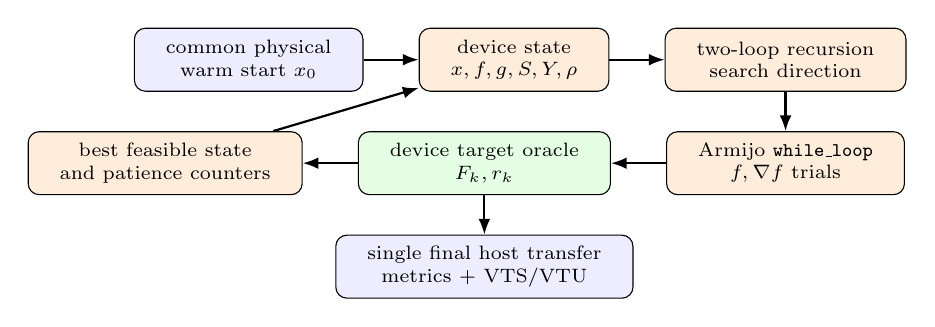
\begin{tikzpicture}[
  node distance=5mm and 7mm,
  box/.style={draw,rounded corners,align=center,minimum height=8mm,
              inner xsep=4mm,fill=blue!7,font=\scriptsize},
  gpu/.style={box,fill=orange!14},
  check/.style={box,fill=green!10},
  flow/.style={-{Latex[length=2mm]},thick}
]
\node[box] (warm) {common physical\\warm start $x_0$};
\node[gpu,right=of warm] (state) {device state\\$x,f,g,S,Y,\rho$};
\node[gpu,right=of state] (loop) {two-loop recursion\\search direction};
\node[gpu,below=of loop] (line) {Armijo \code{while\_loop}\\$f,\nabla f$ trials};
\node[check,left=of line] (target) {device target oracle\\$F_k,r_k$};
\node[gpu,left=of target] (select) {best feasible state\\and patience counters};
\node[box,below=of target] (host) {single final host transfer\\metrics + VTS/VTU};
\draw[flow] (warm) -- (state);
\draw[flow] (state) -- (loop);
\draw[flow] (loop) -- (line);
\draw[flow] (line) -- (target);
\draw[flow] (target) -- (select);
\draw[flow] (select) -- (state);
\draw[flow] (target) -- (host);
\end{tikzpicture}
\caption{Schema-4 device solver boundary.  The orange and green iteration path
is one compiled accelerator executable; it has zero per-iteration host
callbacks.  CPU/GPU SciPy baselines use the same warm start and target policy.}
\label{fig:device-lbfgs-architecture}
\end{figure}

The device implementation is L-BFGS rather than a general replacement for
bounded L-BFGS-B.  The current coil refinement supplies no active variable
bounds, so this is a matched comparison for the present experiment; future
bounded problems require a projected-gradient and generalized-Cauchy-point
extension.  The line search enforces sufficient decrease but not SciPy's strong
Wolfe condition.  Consequently the iteration trajectory and evaluation count
may differ even with an identical start.  That difference is acceptable only
when the exported quantities of interest independently pass the 10\% target
contract and remain within 10\% of the CPU reference.

\subsection{Schema-4 qualification contract and decision}

The result now stores three complete final metric sets: CPU SciPy, GPU SciPy,
and device GPU.  Each contains objective, quadratic flux, mean/RMS/maximum
$|B\cdot n|/|B|$, and all coil-constraint measurements.  Each final surface is
exported as VTS with signed and absolute normalized normal field, and each
symmetry-expanded coil set as VTU.  The analyzer validates device residency and
zero host callbacks, plots all three accepted-checkpoint trajectories and solve
times, and compares the device surface to the CPU-oracle surface.  Compilation
time remains separate from warm execution time.

\textbf{Decision.}  Run the updated engineering Colab notebook and return
\code{simsopt-device-lbfgs.zip}.  Qualification requires the three exported
designs to satisfy the $1.1\times10^{-5}$ flux boundary and every one-sided
engineering envelope.  Device-versus-CPU quantities of interest must agree
within 10\%.  Speedup is reported only after these scientific gates; failure is
still preserved as diagnostic data rather than hidden.  No schema-4 performance
or convergence claim is made in this report until the NVIDIA archive is
analyzed.

\subsection{Measured schema-4 A100 qualification}

The returned archive has SHA-256
\code{476c1a08761dd92f3a50a16bdf126bd210c2226cdabdd6ad5e86b750498c53f8}
and was produced from commit \code{c502c1630f8f10fe805c801cc6ffb4c50f419aa2}.
The analyzer validated the schema and all six VTS/VTU files.  The run used an
NVIDIA A100-SXM4-40GB, JAX~0.11.1 in float64, SciPy~1.16.3, target/source tile
sizes 1024/1920, and the custom Biot--Savart VJP.  All three exported designs
pass the quadratic-flux target and every one-sided 10\% engineering envelope;
hence the result is scientifically validated under the project rule.

\begin{table}[htbp]
\centering
\caption{Independent SIMSOPT CPU-oracle metrics for the three schema-4
checkpoints.  All values pass their physical target envelopes.}
\label{tab:device-lbfgs-qoi}
\small
\begin{tabular}{lrrr}
\toprule
Quantity & CPU SciPy & GPU SciPy & device GPU \\
\midrule
Quadratic flux & $8.61564\times10^{-7}$ & $8.61564\times10^{-7}$ & $7.56845\times10^{-7}$ \\
Normalized field mean & 0.00135658 & 0.00135658 & 0.00128958 \\
Normalized field RMS & 0.00174133 & 0.00174133 & 0.00163524 \\
Normalized field maximum & 0.00611851 & 0.00611851 & 0.00573712 \\
Minimum coil--coil distance (m) & 0.139627 & 0.139627 & 0.144844 \\
Minimum coil--surface distance (m) & 0.280193 & 0.280193 & 0.271117 \\
Maximum curvature (m$^{-1}$) & 5.03888 & 5.03888 & 4.81980 \\
Maximum MSC (m$^{-2}$) & 5.47919 & 5.47919 & 5.15408 \\
Total base-coil length (m) & 17.8202 & 17.8202 & 17.6366 \\
Recorded objective & $1.07673\times10^{-4}$ & $1.07673\times10^{-4}$ & $2.69450\times10^{-4}$ \\
\bottomrule
\end{tabular}
\end{table}

The device result is not merely a numerically perturbed copy of the SciPy
checkpoint.  Relative to CPU SciPy it lowers quadratic flux by 12.2\%, field
RMS by 6.09\%, maximum curvature by 4.35\%, maximum MSC by 5.93\%, and length
by 1.03\%.  Its minimum coil--surface distance is 3.24\% lower, at 0.271117~m,
but remains just inside the allowed 0.27~m boundary.  The scalar recorded
objective is 150.25\% higher, so the independent device-versus-CPU objective
agreement gate fails.  It is the only failed acceptance gate.  This does not
invalidate the design under the explicit target-based scientific policy, but
it proves that Armijo L-BFGS and strong-Wolfe L-BFGS-B reached different valid
trade-offs in the nonconvex envelope.  Therefore the device solver is qualified
for scientific feasibility, not yet as a trajectory-equivalent drop-in
replacement.

\begin{figure}[htbp]
\centering
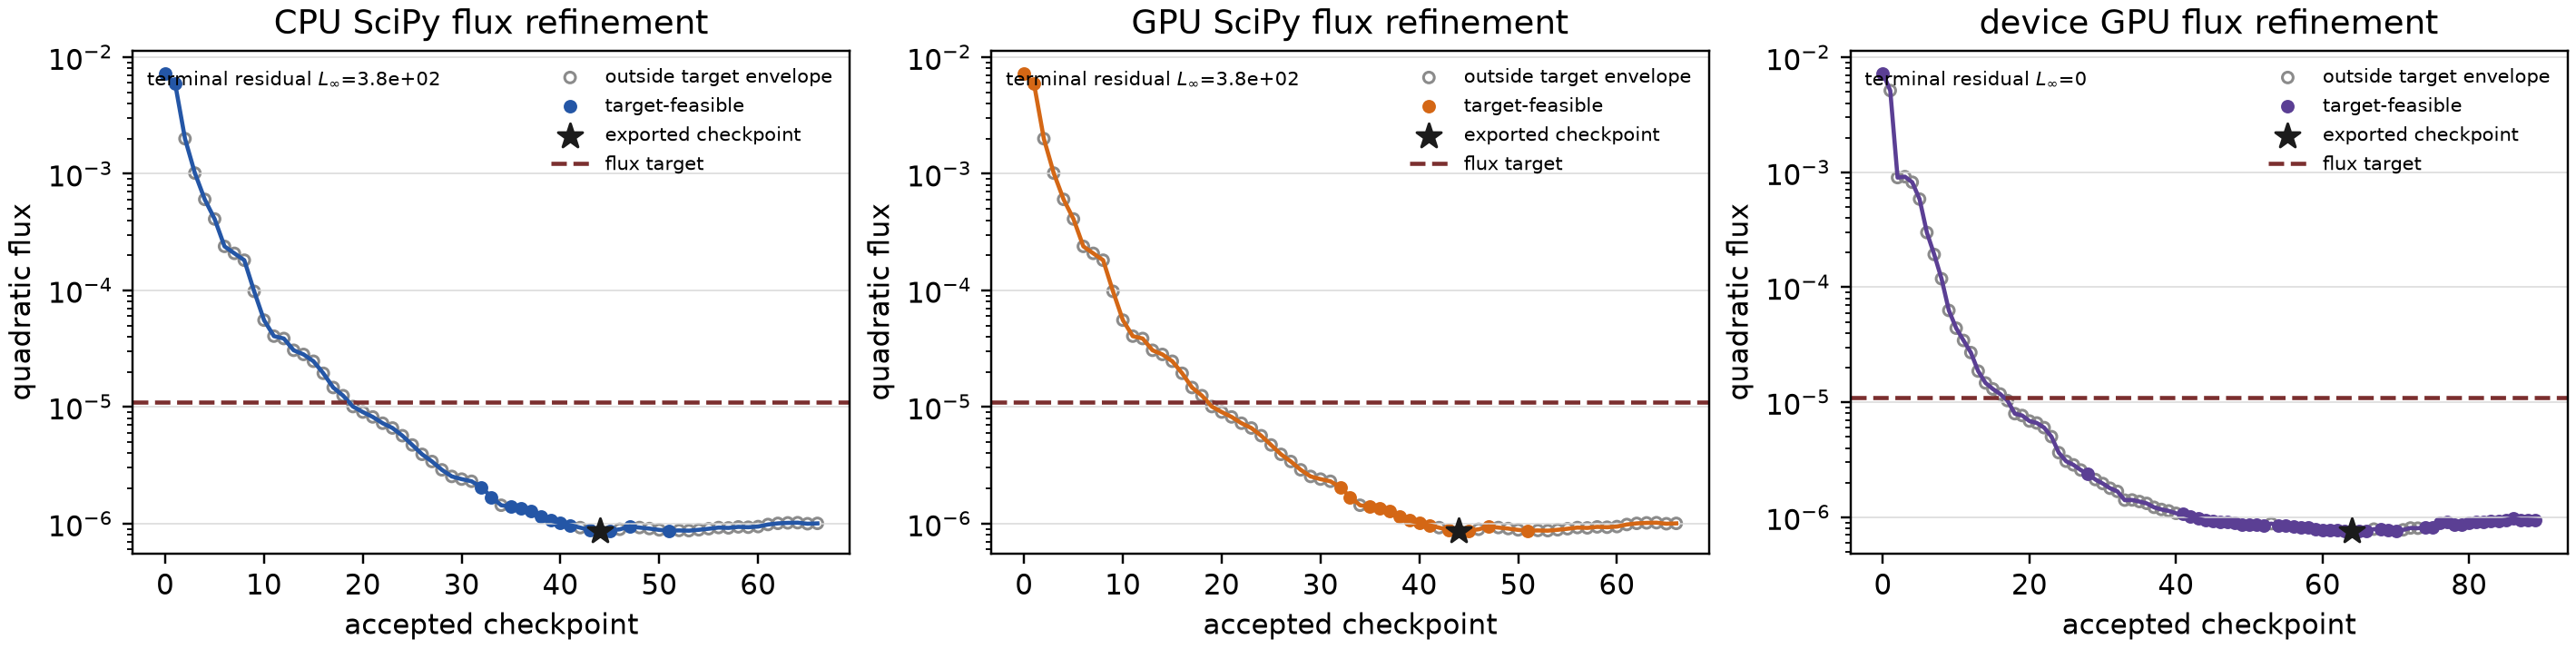
\includegraphics[width=\textwidth]{figures/device_lbfgs_comparison_trajectory.png}
\caption{Accepted-checkpoint trajectories for the matched CPU SciPy, GPU SciPy,
and device-GPU refinements.  Filled points satisfy the engineering envelope;
stars mark the exported states.  SciPy selects checkpoint~44, while device
L-BFGS follows a distinct path and selects checkpoint~64.}
\label{fig:device-lbfgs-trajectory}
\end{figure}

Target-aware stopping preserves the schema-3 SciPy design exactly while
eliminating 534 of 600 iterations.  Both SciPy runs first satisfy the flux and
engineering targets at checkpoint~32, select their minimum-flux feasible state
at checkpoint~44, and stop at iteration~66 after 15 consecutive infeasible
accepted states.  Their 75 objective/gradient evaluations take 58.428~s on CPU
and 0.6940~s on GPU.  Compared with the preceding 600-iteration measurements
of 501.69~s and 5.974~s, target awareness reduces refinement time by about
$8.59\times$ and $8.61\times$, respectively, without changing the exported
quality.

Device L-BFGS first reaches the joint target at checkpoint~28, selects
checkpoint~64, and stops at iteration~89 after its 25-checkpoint significant-
improvement patience expires.  It performs 92 objective/gradient evaluations
in 0.7468~s.  Warm execution is therefore 0.929$\times$ the speed of host-driven
GPU SciPy---7.59\% slower overall---because it performs 22.7\% more evaluations.
Per physics evaluation it is 1.140$\times$ faster, direct evidence that removing
host callbacks reduces steady-state overhead.  Compilation changes the
first-call result: GPU SciPy objective plus quality compilation takes 7.583~s,
whereas the fused device solver compiles in 3.931~s.  Including solve time, the
device first call takes 4.677~s versus 8.277~s for GPU SciPy, a
1.770$\times$ speedup; it is 13.289$\times$ faster than the analogous CPU first
call.

\begin{figure}[htbp]
\centering
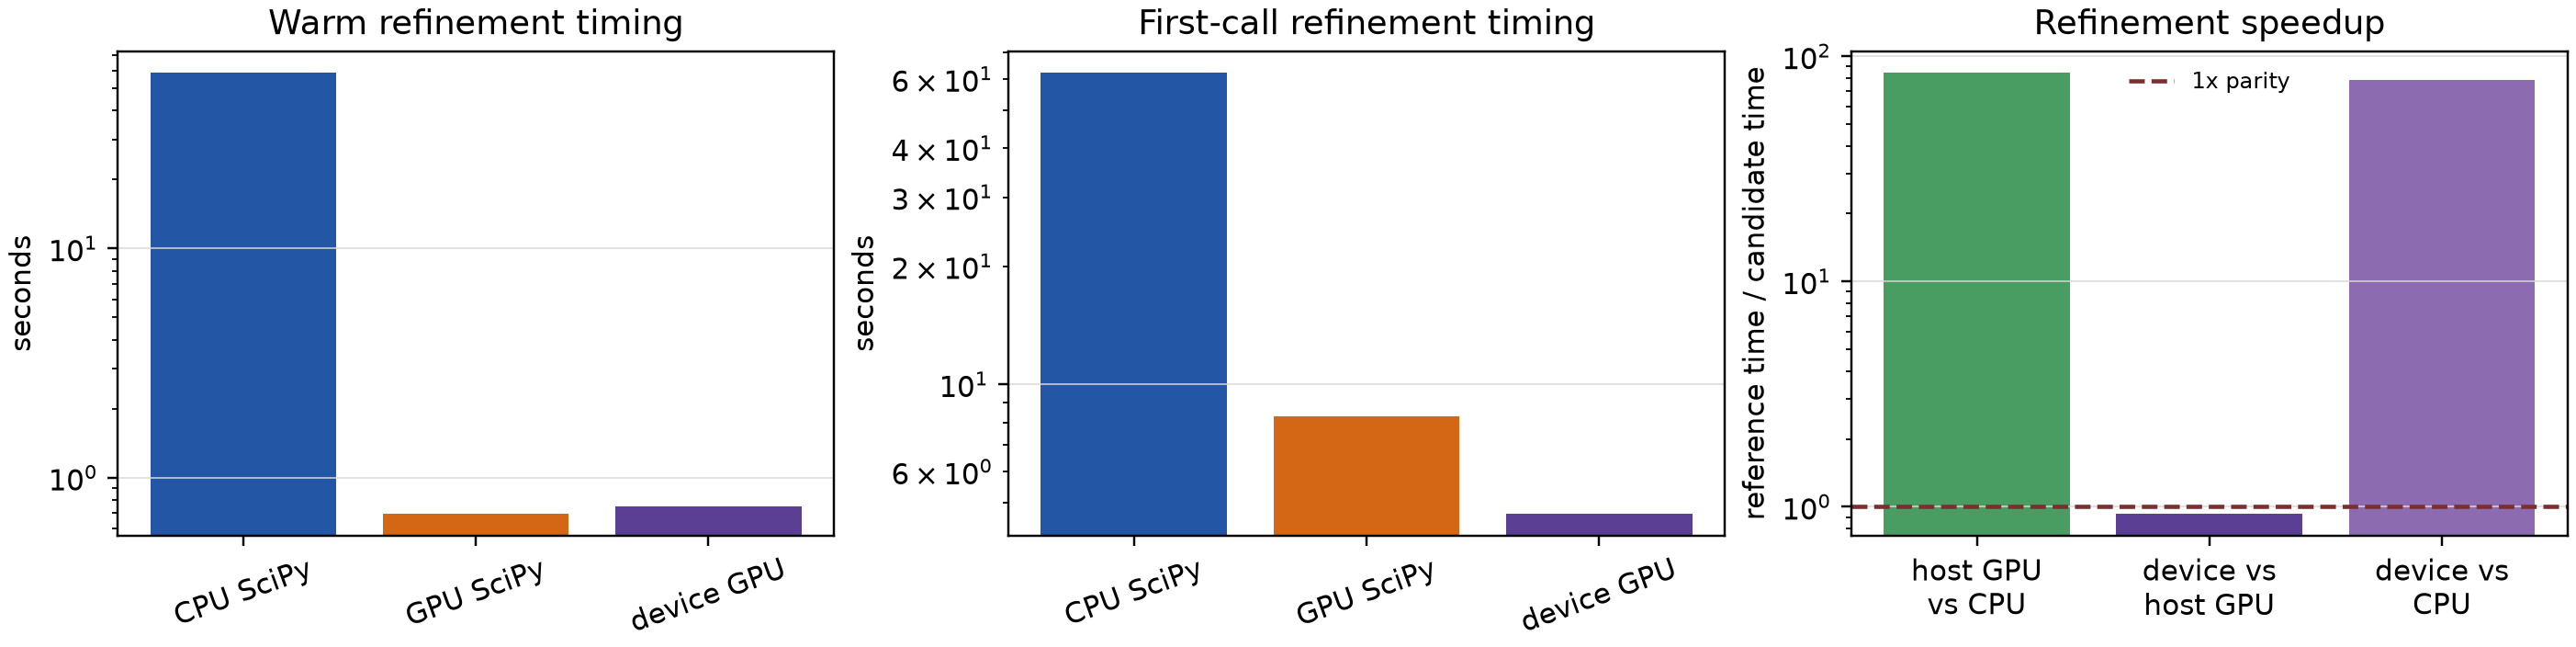
\includegraphics[width=\textwidth]{figures/device_lbfgs_comparison_performance.png}
\caption{Matched refinement performance.  Warm solve time, compilation-inclusive
first-call time, and solver-to-solver speedups are separated.  Device residency
wins per evaluation and on first call, but its longer Armijo trajectory loses
slightly to warm GPU SciPy.}
\label{fig:device-lbfgs-performance}
\end{figure}

\begin{figure}[htbp]
\centering
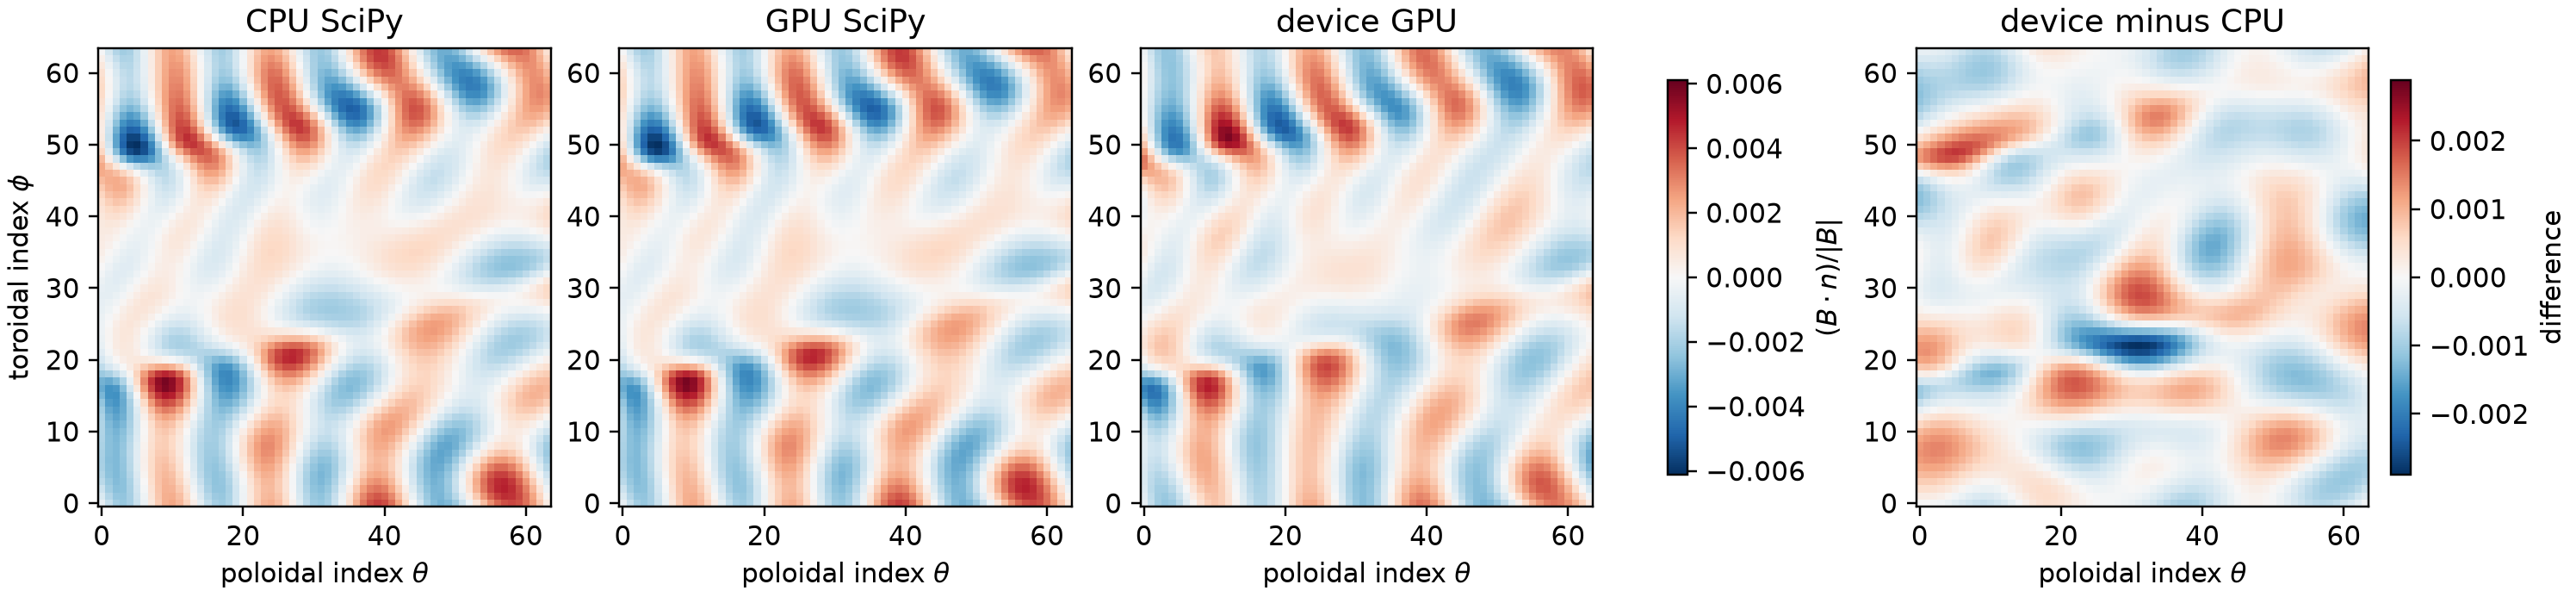
\includegraphics[width=\textwidth]{figures/device_lbfgs_comparison_surface.png}
\caption{Signed $(B\cdot n)/|B|$ from the three exported surface VTS files.
CPU/GPU SciPy remain identical to plotting accuracy.  The device design has
signed-field correlation 0.9234 with CPU, relative $L^2$ difference 0.3844,
and maximum pointwise difference 0.002891, consistent with a different valid
optimization basin rather than a backend-parity error.}
\label{fig:device-lbfgs-surface}
\end{figure}

\textbf{Decision.}  Accept target-aware stopping immediately: it gives an
order-of-magnitude refinement reduction with no loss of the selected SciPy
design.  Retain device L-BFGS as an experimental qualified solver, but do not
replace GPU SciPy for repeated warm solves yet.  The next solver study should
replay the qualified common warm start across history sizes and target-patience
values, then add a device strong-Wolfe line search if trajectory length or
objective trade-off does not improve.  The optimization target remains the
actual flux and coil quantities, while the scalar objective and full surface
map remain mandatory diagnostics against accidental trade-off degradation.

\paragraph{Iteration and geometry clarification.}
The engineering qualification configures at most eight augmented-Lagrangian
outer stages and 300 L-BFGS-B iterations per inner solve.  The measured CPU and
GPU AL runs actually terminate after only two outer stages because the second
inner solve reaches its 300-iteration cap without satisfying the stationarity
safeguard.  CPU inner stages use 121 and 300 iterations (421 total); GPU stages
use 24 and 300 (324 total).  The subsequent direct-flux refinement is a separate
optimization, not another AL outer stage: target awareness stops SciPy at 66
iterations and device L-BFGS at 89 from a nominal 600-iteration allowance.

The problem begins with four unique \code{CurveXYZFourier} base coils of order
eight and 120 quadrature points per coil.  Each Cartesian coordinate has
$2(8)+1=17$ Fourier coefficients, giving 51 geometric degrees of freedom per
coil, 204 curve variables, and three free currents: 207 optimization variables.
The initial curves are equally spaced circles with major radius 1.0~m and coil
radius 0.5~m.  Only their first harmonic is initially nonzero; the unused modes
through order eight allow the optimizer to deform them.  Field-period and
stellarator symmetry expand the four independent curves to sixteen physical
coils.

\subsection{Implemented warm-start replay study}

The next qualification code now removes the AL phase from solver-parameter
experiments.  The schema-4 analyzer preserves the selected AL endpoint as a
207-entry physical-coordinate warm start together with its archive hash and
CPU/GPU reference metrics.  A dedicated replay benchmark reconstructs the
same engineering problem, verifies the saved dimension and scientific
provenance, and evaluates the Cartesian product

\[
  m\in\{10,20,50,100\},\qquad
  p\in\{15,25\},
\]

where $m$ is L-BFGS history size and $p$ is significant-improvement checkpoint
patience.  All eight candidates use the same infeasible patience 15, maximum
150 iterations, Armijo line-search budget 30, float64 objective, target oracle,
and physical warm start.  Each solver is compiled independently so history-
shape compilation is included explicitly, while warm solve time remains
separate.

Every candidate records its complete accepted-checkpoint trajectory and final
CPU-oracle objective, quadratic flux, normalized-normal-field metrics, currents,
coil lengths, distances, curvature, and mean-squared curvature.  Scientific
qualification still requires flux and all physical engineering envelopes.
Ranking first prefers scientifically valid candidates whose recorded objective
is within 10\% of the CPU SciPy reference, then chooses minimum quadratic flux,
warm time, and stable configuration name.  The winner alone is exported as VTS
and VTU.  This hierarchy prevents a history-size sweep from winning merely by
following the schema-4 device trajectory to a substantially different scalar
trade-off.

The Colab workflow runs only this replay grid and should therefore finish much
faster than a complete AL qualification.  Its archive is named
\code{simsopt-device-lbfgs-replay.zip}.  The analyzer will produce a four-panel
history/patience grid and overlaid flux trajectories.  No configuration choice
is promoted until those NVIDIA measurements and final physical targets are
returned and added to this report.

\section{Opportunities to improve coil quality}

GPU acceleration is valuable because it enables better algorithms, not only
shorter repetitions.  Once the first objective is validated, the following
experiments have high priority:
\begin{enumerate}
  \item \textbf{Multiresolution continuation:} increase surface resolution,
        coil quadrature, and Fourier order as optimization progresses.
  \item \textbf{Batched multistart:} use accelerator parallelism to explore
        multiple initial coil sets for the nonconvex problem.
  \item \textbf{Variable projection of currents:} exploit the linear dependence
        of $B$ on free currents and solve the small conditional least-squares
        problem inside each geometry evaluation where the objective permits it.
  \item \textbf{Residual-form methods:} expose $B\cdot n$ and engineering
        residuals for matrix-free Gauss--Newton or Levenberg--Marquardt.
  \item \textbf{Scaling and preconditioning:} nondimensionalize currents,
        positions, Fourier modes, and penalty families so that line searches and
        curvature approximations operate on comparable scales.
  \item \textbf{Constraint handling:} investigate augmented-Lagrangian or
        constrained formulations for minimum distance and maximum curvature in
        place of increasingly ill-conditioned penalty weights.
\end{enumerate}

\section{Risk register}

{\scriptsize
\begin{longtable}{p{0.24\textwidth}p{0.32\textwidth}p{0.36\textwidth}}
\toprule
Risk & Consequence & Mitigation \\
\midrule
Insufficient GPU problem size & Launch and compilation costs erase gains & Keep
  the SciPy/CPU backend; judge success on production-sized cases; batch solves
  where scientifically useful. \\
Poor float64 throughput & Fast float32 results fail scientific tolerances & Use
  data-center/HPC GPUs for the primary benchmark; validate any mixed-precision
  path against float64. \\
Reverse-mode memory growth & Out-of-memory failures at high resolution & Tile
  interactions, use a custom VJP, rematerialize, and benchmark peak memory. \\
Dynamic neighbor lists & Recompilation or incorrect distance gradients & Use an
  all-pairs reference and fixed-capacity masked lists with explicit refresh
  semantics. \\
Reduction-order differences & CPU/GPU values disagree near strict tolerances &
  Use scale-aware tests, compensated/pairwise reductions where necessary, and
  compare physical metrics as well as bit-level outputs. \\
Hybrid host/device code & Hidden synchronization prevents speedup & Inspect
  traces and forbid callbacks in the steady-state objective. \\
Upstream divergence & Long-lived fork becomes difficult to merge & Keep changes
  modular, rebase at planned integration points, and propose focused upstream
  pull requests. \\
Solver trajectory changes & Backend appears faster but converges worse & Retain
  SciPy and identical starting points until objective parity is complete; count
  physics evaluations in every comparison. \\
\bottomrule
\end{longtable}
}

\section{Version-control workflow}

The long-lived integration branch is \code{gpu-native-objective}.  Work should
arrive through short, focused branches.  Commits keep code, tests, and benchmark
changes reviewable; generated data and PDFs remain uncommitted unless selected
as release artifacts.  Each pull request records the numerical contract,
hardware and precision, parity tolerances, synchronized warm/cold timings, peak
memory, profiler evidence, and unsupported terms.  Integration will periodically
rebase on or merge a pinned \code{upstream/master} without force-updating the
fork's existing \code{master} branch.

\section{Documentation policy}

This is a living engineering report, not a fixed-length deliverable.  New
measurements, convergence plots, profiler evidence, visualizations, rejected
alternatives, and implementation decisions will be retained whenever they help
explain the state of the project.  Concision remains useful, but there is no
nine-page limit.  The report concentrates on project-specific implementation
evidence and decisions.

\paragraph{References.}

{\scriptsize
[1] \href{https://github.com/hiddenSymmetries/simsopt}{SIMSOPT repository}.
[2] \href{https://simsopt.readthedocs.io/latest/example_coils.html}{SIMSOPT coil
optimization documentation}.
[3] \href{https://docs.jax.dev/en/latest/default_dtypes.html}{JAX, ``Default
dtypes and the X64 flag.''}
[4] \href{https://docs.jax.dev/en/latest/benchmarking.html}{JAX,
``Benchmarking JAX code.''}
[5] \href{https://optax.readthedocs.io/en/latest/_collections/examples/lbfgs.html}{Optax,
``L-BFGS.''}
}

\end{document}
